\documentclass[11pt,a4paper]{article}
\usepackage[italian]{babel}
\usepackage[T1]{fontenc}
\usepackage[utf8]{inputenc}
\usepackage{graphicx}
\usepackage{imakeidx}
\usepackage{amsmath}
\makeindex[intoc]
\usepackage[hyperfootnotes=false, colorlinks=true, linkcolor=black]{hyperref}
\usepackage{verbatim}


\begin{document}
\title{Reti e sistemi operativi - Reti}
\author{Jacopo De Angelis}
\maketitle
\tableofcontents
\pagebreak

\begin{LARGE}
Programma esteso
\end{LARGE}
\begin{itemize}
\item {Introduzione e cenni al livello fisico} \textit{cap. 1.1 - 1.5 (no 1.3.2)} 
\item Livello di trasporto \textit{cap. 3 (no 3.6.2 e 3.7.2)}:
	\begin{itemize}
		\item funzioni del livello di trasporto
		\item trasporto UDP
		\item trasporto TCP
		\item controllo della congestione
	\end{itemize}
\item Livello di rete \textit{cap. 4.1, 4.3 (no 4.3.5), 5.2, 5.6}:
	\begin{itemize}
		\item funzioni del livello di rete
		\item indirizzamento IP
		\item algoritmi di instradamento
	\end{itemize}
\item LAN, Wireless LAN, Elementi di livello fisico \textit{cap. 6.1, 6.2, 6.3 (no 6.3.4), 6.4, 7.1, 7.2 (no 7.2.1), 7.3 (no 7.3.6)} :
	\begin{itemize}
		\item funzioni del livello di collegamento
		\item CSMA/CD e LAN Ethernet
	\end{itemize}
\end{itemize}

\pagebreak
\section{Reti di calcolatori e internet}
\subsection{Che cos'è internet?}
\subsubsection{Una descrizione pratica}
Internet è una rete pubblica di calcolatori sparsi in tutto il mondo. I terminali sono collegatri tra di loro attraverso link di comunicazione, diversi link possono trasmettere i dati a differenti velocità. Questa velocità è chiamata “larghezza di banda” e di solito si misura in bit/secondo. \\
Solitamente i terminali sono collegati indirettamente attraverso dispositivi di comunicazione detti router. Un router preleva le informazioni che arrivano tramite uno di questi link in ingresso e lo reindirizza a un link in uscita. Queste informazioni sono chiamate “pacchetti”. Il tragitto del pacchetto da è detto route o path. Internet usa una tecnica conosciuta come “commutazione di pacchetto” (packet switching) che permette a più terminali di condividere un cammino o anche solo parte di questo.
I terminali accedono a internet attraverso gli ISP (Internet Service Providers). Ogni ISP è una serie di router e di link di comunicazione. \\
I terminali eseguono protocolli di comunicazione che controllano l’invio e la ricezione di informazioni all’interno di internet. Due dei più importanti sono il TCP (Transmission Control Protocol) e l’IP (Internet Protocol). Il protocollo IP specifica il formato dei pacchetti che sono scambiati fra router e fra terminali.

\subsubsection{Descrizione del servizio}
Internet permette la distribuzione delle applicazioni che girano sui suoi terminali per scambiare dati fra le diverse unità.
Internet fornisce due servizi per le applicazioni da esso distribuite: un servizio orientato alla connesione e un servizio senza connessione. Il primo garantisce che i dati trasmessi saranno consegnati al destinatario nella loro integrità, il secondo invece risulta inaffidabile.

\subsubsection{Che cos'è un protocollo?}
Un protocollo definisce il formato e l’ordine dei messaggi scambiati tra due o più entità comunicanti, così come le azioni che hanno luogo a seguito della trasmissione e/o ricezione di un messaggio o di altri eventi.

\subsection{La sezione di accesso alla rete}
\subsubsection{Terminali, client e server}
I computer colelgati a internet sono spesso chiamati host o end-system (“terminali”). Ci si riferisce a essi come terminali perché sono collocati nella sezione di accesso a internet. Il termine host (ospite) deriva dal fatto che ospitano (eseguono) programmi di livello applicativo come i browser o simili. \\
Gli host, a volte, sono suddivisi in due categorie:
\begin{itemize}
	\item Client
	\item Server
\end{itemize}
Un programma client è un programma che gira su un terminale che richiedere e riceve un servizio da un programma server che gira su un altro terminale.
Poiché, tipicamente, un client gira su un calcolatore mentre il server gira su un altro, le applicazioni client/server in internet sono, per definizione, applicazioni distribuite.
\begin{figure}
	\begin{center}
		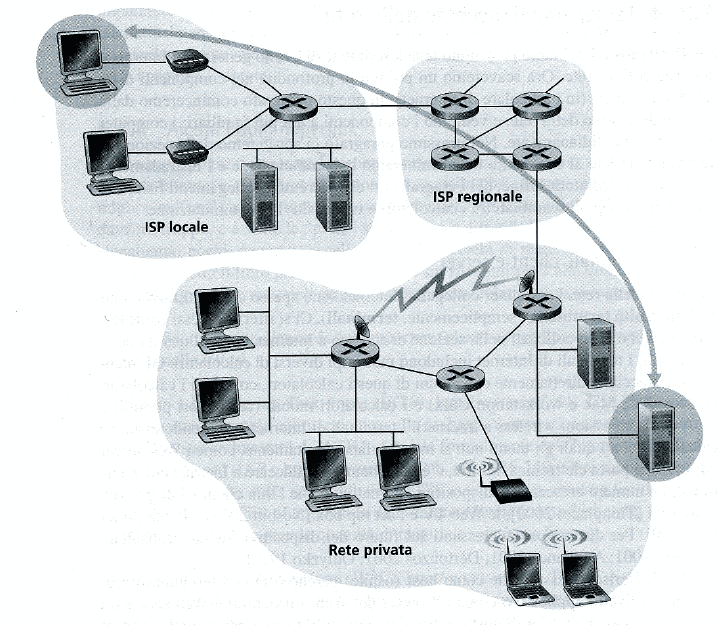
\includegraphics[scale=0.6]{img/001.png}
	\end{center}
\end{figure}
A questo livello di astrazione i router, i link e altri “componenti” di internet servono come “scatola nera” che trasferisce messaggi tra i diversi componenti per la comunicazione in internet.

\subsubsection{Servizio senza connessione e servizio orientato alla connessione}
Le reti TCP/IP, e in particolare internet, forniscono due tipi di servizio per le sue applicazioni:
\begin{itemize}
	\item Un servizio senza connessione
	\item Un servizio orientato alla connessione
\end{itemize}
Chi crea un’applicazione internet deve programmare l’applicazione per l’impiego di uno di questi due servizi.
\paragraph{Servizio orientato alla connessione}
\textbf{Il client e il server (residenti in due diversi terminali) si scambiano pacchetti di controllo prima di spedire i pacchetti contenenti i dati reali.} Queste procedure di “stretta di mano” (handshaking procedure), allertano client e server, permettendo loro di prepararsi per l’arrivo massiccio dei pacchetti. Una volta terminata questa procedura la connessione tra i due terminali è instaurata. \\
Perché si utilizza la terminologia “servizio ORIENTATO alla connessione” e non semplicemente “servizio di connessione”? Questo perché solo i due terminali sono coscienti della connessione, all’interno della rete i commutatori sono ignari della connessione e non mantengono informazioni sullo stato della connessione.
Il servizio orientato alla connessione di internet è raggruppato con molti altri servizi:
\begin{itemize}
	\item \textbf{Trasferimento di dati affidabile}: un’applicazione può affidarsi a una connessione per consegnare tutti i suoi dati senza errori o nell’ordine appropriato. Questa affidabilità deriva dall’impiego di segnali di riscontro e ritrasmissioni.
	\item \textbf{Controllo di flusso}: assicura che nessuna delle due estremità saturi l’altra con l’invio a velocità eccessiva di troppi pacchetti.
	\item \textbf{Controllo della congestione}: previene che internet entri nello stato di blocco incrociato (gridlock), ovvero quando un router è congestionato e rischia di perdere pacchetti. In questa circostanza, se le velocità di comunicazione continuano a riempire la rete troppo velocemente, i pacchetti saranno persi per la maggior parte. Internet evita questo problema costringendo i terminali a ridurre la velocità di invio durante i periodi di congestione, riscontrata grazie alla mancanza dei messaggi di riscontro.
\end{itemize}
\textbf{Il servizio orientato alla connessione di internet ha un nome: TCP (Transmission Control protocol).}
\paragraph{Servizio senza connessione}
\textbf{Non esiste handshake.} Quando un’estremità di un’applicazione vuole inviare pacchetti a un’altra, semplicemente, li invia. Poiché manca l’handshake l’invio sarà più veloce ma non esisterà un messaggio di riscontro dell’avvenuta ricezione.
\textbf{Il servizio di internet senza connessione è l’UDP (User Datagram Protocol).}

\subsection{Il nucleo della rete}
\subsubsection{Commutazione di circuito e commutazione di pacchetto}
Esistono due principali tipi di approccio per la costruzione della sezione interna di una rete:
\begin{itemize}
	\item l\textbf{a commutazione di circuito} (circuit switching): le risorse necessarie lungo un percorso per fornire la comunicazione fra due terminali sono riservate per la durata della sessione.
	\item \textbf{la commutazione di pacchetto} (packet switching): le risorse non sono riservate, i messaggi della sessione utilizzano le risorse a richiesta e, di conseguenza, devono aspettare per accedere al link di comunicazione.
\end{itemize}
Le reti telefoniche sono un esempio di rete a commutazione di circuito. Internet, invece, è un esempio di rete a commutazione di pacchetto. Le reti non sono per forza o di un tipo o dell’altro.

\begin{comment}
\subsubsection{Commutazione di circuito}
Nell’immagine qua accanto i quattro commutatori di circuito sono collegati da due link. Ognuno di questi link è costitutito da n circuiti, in modo che ciascun link possa mantenere n connessioni simultanee.
I terminali sono collegati direttamente a uno dei commutatori. Alcuni degli host hanno un accesso analogico ai commutatori, mentre altri hanno un accesso numerico diretto. Per l’accesso analogico è necessario un modem. Quando due host desiderano comunicare, la rete stabilisce un circuito dedicato end-to-end fra essi. In questo caso viene prenotato un circuito su ciascuno dei due link.
\begin{figure}
	\begin{center}
		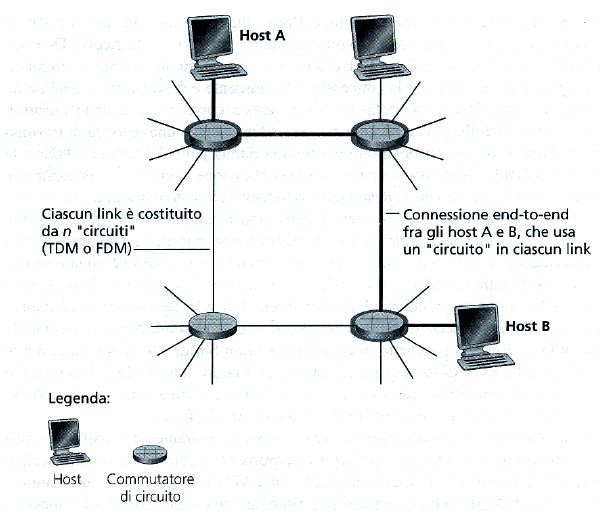
\includegraphics[scale=0.6]{img/002.png}
		\caption{Una semplice rete a commutazione di circuito, che consiste di quattro commutatori di circuito collegati da quattro link}
	\end{center}
\end{figure}
\paragraph{Multiplazione (multiplexing) nelle reti a commutazione di circuito)} \label{par: 001}
Un circuito in un link è realizzato mediante la multiplazione a divisione di frequenza (FDM) o la multiplazione a divisione di tempo (TDM).
Con l’FDM, lo spettro di frequenza di un link è diviso fra le connessioni stabilite sul link, dedicando così una banda di frequenza. \\
Per il TDM il dominio temporale è suddiviso tra quattro circuiti con quattro time slot in ciascun frame; a ciuacun circuito è assegnato lo stesso slot nei frame TDM che si succedono. La velocità di trasmissione di ciascun circuito è uguale a:
\begin{center}
	\textit{velocità del frame * numero di bit in uno slot}
\end{center}

\begin{figure}
	\begin{center}
		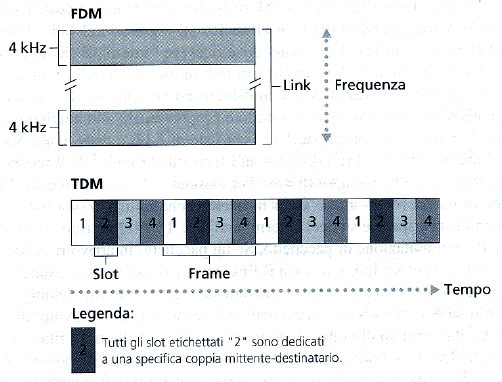
\includegraphics[scale=0.7]{img/003.png}
		\caption{Con L'FDM ciascun circuito occupa continuamente una frazione della larghezza di banda. Con il TDM ciascun circuito occupa periodicamente tutta la larghezza di banda durante brevi intervalli di tempo (durante gli slot)}
	\end{center}
\end{figure}

per esempio, se il link trasmette 8000 frame al secondo e ogni slot è costituito da 8 bit, la velocità di trasmissione è 64 Kb/s. \\
I fautori della commutazione di pacchetto hanno sempre sostenuto che la commutazione di circuito porta a sprechi, perché i circuiti dedicati sono 	inattivi durante i periodi silenti (ad esempio quando la linea telefonica non viene usata).
\end{comment}

\paragraph{Commutazione di pacchetto}
\textbf{Nelle moderne reti di calcolatori, la sorgente suddivide i messaggi lunghi in pezzi più piccoli di dati conosciuti come paccehtti.} \\
Fra sorgente e destinazione ciascuno di questi pacchetti viaggia lungo link di comunicazione e commutatori di pacchetto (router). I pacchetti sono trasferiti sulla linea con velocità massima rispetto a quella del link. \\
Molti router utilizzano la \textbf{trasmissione “store and forward”} all’ingresso dei link, ovvero che il router deve ricevere l’intero pacchetto prima di poter cominciare a trasmettere il primo bit sul link in uscita. Quindi i router store and forward introducono un ritardo store and forward all’ingresso di ciascun link. Questo ritardo è proporzionale alla lunghezza in bit del pacchetto, in particolare un pacchetto di L bit inoltrato su di un link in uscita a R bit/s ci metterà un ritardo di L/R secondi.
Ogni router è collegato a molti link. Per ciascun link cui è collegato il router ha un buffer di uscita che immagazzina pacchetti che il router si appresta a spedire su quel determinato link. Nel caso un pacchetto in uscita trovi il link occupato, dovrà attendere che il pacchetto precedente venga spedito, aggiungendo così un ulteriore ritardo chiamato “ritardo di coda”. L’entità di questo ritardo è variabile ed è dipendente dalla congestione della rete. In certi casi si può anche perdere pacchetti, sia in arrivo che in uscita. \\
La commutazione di pacchetto impiega la multiplazione statistica, in netto contrasto con la multiplazione a divisione di tempo. In questo caso, infatti, i pacchetti vengono spediti in ordine di arrivo.
Ora proviamo a calcolare il tempo che occorre ad inviare un pacchetto di L bit da un host all’altro attraverso una rete a commutazione di pacchetto. Supponiamo che esistano Q link fra i due host, ciascuno con velocità R bit/s. assumiamo ritardi dovuti a coda e propagazione end-to-end trascurabili e che non sia stabilita alcuna connessione (niente handshake). Il pacchetto dovrà passare per Q-1 link, quindi dovrà essere trasmesso Q-1 volte. Essendo il tempo richiesto dallo store and forward L/R, il tempo totale sarà \textbf{Q(L/R)}.
\paragraph{Frammentazione del messaggio}
In una moderna rete a commutazione di pacchetto, la sorgente frammenta i lunghi messaggi dello strato di applicazione in pacchetti più piccoli e invia questi ultimi nella rete. Sebbene la frammentazione complichi la vita di sorgente e destinatario, si è concluso che i vantaggi compensano grandemente gli svantaggi.
Diciamo che una rete a commutazione di pacchetto effettua una commutazione di messaggio se le sorgenti non frammentano i messaggi.
Quando invece un messaggio viene segmentato in pacchetti, si dice che la rete effettua in pipeline la trasmissione dei messaggi, cioè parti del messaggio vengono trasmesse in parallelo dalla sorgente e dai commutatori di pacchetto.
Un vantaggio della commutazione di pacchetto con segmentazione è che il ritardo della connessione end-to-end è molto ridotto. Con le immagini accanto si può capire perché i tempi siano più rapidi, è infatti il vantaggio della pipeline. \\
Per fare un esempio, consideriamo un messaggio lungo $7,5 * 10^{6}$ bit. Supponiamo che tra i due host ci siano due commutatori di pacchetto e tre link, ciascun link abbia una velocità di trasmissione di 1,5 Mbit/s ($1,5 * 10^{6} bit$). Assumendo che la rete non sia in congestione, quanto tempo è richiesto per trasferire il messaggio con la \textbf{commutazione di messaggio}? Alla sorgente occorrono 5 secondi ($7,5 * 10^{6} bit / 1,5 * 10^{6} bit/s$) per portare il messaggio al primo commutatore. Poichè i commutatori sono di tipo store-and-forward, il primo commutatore deve aspettare tutta la ricezione del pacchetto. Quindi questa procedura si ripete anche tra i commutatori, quindi abbiamo $(7,5 * 10^{6} bit / 1,5 * 10^{6} bit/s)*3 link$. \\
Ora frammentiamo il messaggio in 5000 pacchetti da 1500 bit l'uno. Assumendo che non ci sia congestione, quanto ci metteremo con la \textbf{commutazione di pacchetto}? Occorre 1 ms per spostare il primo pacchetto al primo commutatore ($1,5 * 10^{3} bit / 1,5 * 10^{6} bit/s$), poi 1 ms per ogni link, quindi il primo pacchetto arriverà dopo 3 ms a destinazione. Ora, l'ultimo pacchetto quanto ci metterà? Consideriamo che il secondo pacchetto viene spedito in contemporanea mentre il primo è sul secondo link. Secondo questa logica, l'ultimo pacchetto arriva al primo commutatore dopo $5000 * 1 ms = 5000 ms = 5 s$, quindi dovrà attraversare gli altri due link. Il tempo finale sarà, quindi 5002 ms = 5,002 secondi contro i 15 precedenti. \\
Quindi, la formula è:
\begin{center}
	$d = \dfrac{dim\_pacchetto}{vel\_trasferimento}$
\end{center}	 
\begin{center}	
	$tempo = d * tot\_pacchetti + (link - 1) * d$
\end{center}
Questo miglioramento deriva dal fatto che la commutazione di pacchetto agisce in parallelo.
\begin{figure}
	\begin{center}
		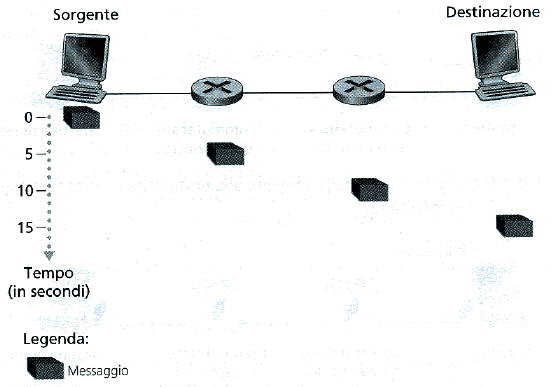
\includegraphics[scale=0.7]{img/004.png}
		\caption{Tempi per il trasferimento del messaggio senza frammentazione dello stesso}
		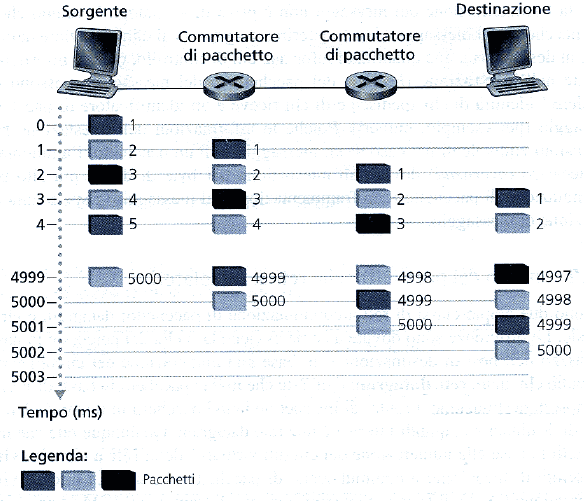
\includegraphics[scale=0.7]{img/005.png}
		\caption{Tempi per il trasferimento del messaggio quando lo stesso è frammentato in 5000 pacchetti}
	\end{center}
\end{figure}
Il vantaggio della segmentazione è anche che nel caso ci sia un errore di bit su di un pacchetto, è il singolo pacchetto a poter essere scartato e non l’intero messaggio.
La frammentazione non è priva di svantaggi, infatti al pacchetto devono essere aggiunte informazioni nell’\textbf{intestazione (header)} e queste possono comprendere l’identità di sorgente e destinatario. In più l’header richiede altri byte di spazio.

\subsection{Accesso alla rete e mezzi trasmissivi}
\subsubsection{Accesso alla rete}
L’accesso può essere classificato in tre categorie:
\begin{itemize}
	\item Accesso domestico
	\item Accesso aziendale
	\item Accesso per terminali mobili
\end{itemize}
Queste categorie, però, non sono rigide e vincolanti.

\subsubsection{Mezzi fisici}
Si dividono in due categorie:
\begin{itemize}
	\item Guidati: guidati attraverso un mezzo solido
	\item Non guidati: si propagano nell’atmosfera
\end{itemize}

\subsection{Gli ISP e la rete dorsale di internet}
\begin{figure}
	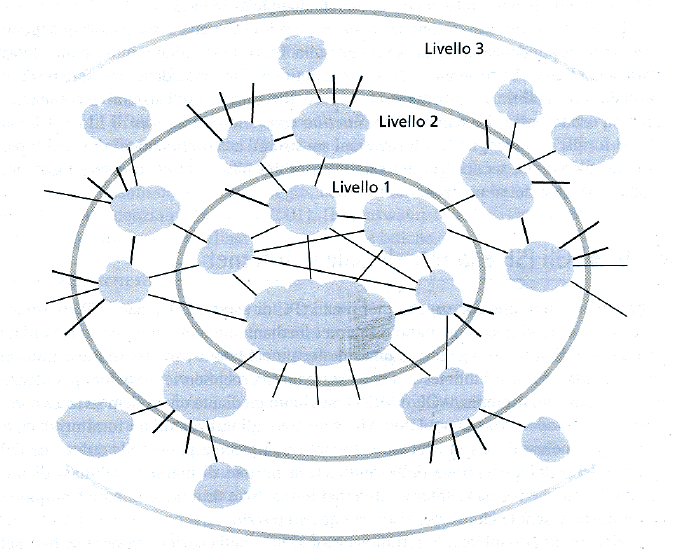
\includegraphics[scale=0.6]{img/006.png}
	\caption{Interconnessione degli ISP}
\end{figure}
Le reti di accesso situate nella sezione esterna di internet sono connesse al resto di internet attraverso una gerarchia a livelli di fornitori di servizi (ISP):
\begin{itemize}
	\item Livello 1: Rete dorsale di internet
	\item Livello 2: Copertura tipicamente regionale o nazionale, connesso a pochi ISP di livello 1.
\end{itemize}
Gli ISP sono in rapporto di utente-fornitore.
Quando due ISP sono collegati direttamente tra di loro sono detti “pari” tra loro.
I punti di collegamento tra i vari ISP sono detti “punti di presenza” (POP).
Gli ISP spesso si connettono in Network Access Point (NAP).

\subsection{Ritardi e perdite nelle reti a commutazione di pacchetto}
\begin{figure}
	\begin{center}
		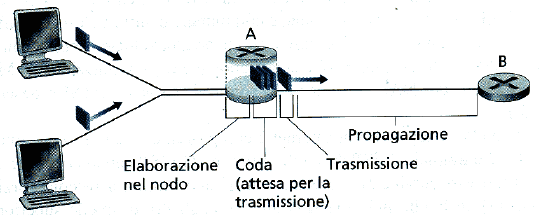
\includegraphics[scale=0.6]{img/007.png}
		\caption{Ritardo al nodo e nel router A}
	\end{center}
\end{figure}
\subsubsection{Tipi di ritardo} \label{par: ritardi}
\paragraph{Ritardo di elaborazione}
Tempo richiesto per esaminare l’intestazione del pacchetto e per determinare dove instradarlo.
Può comprendere altri fattori come il tempo per il controllo degli errori.
Dopo quest’elaborazione, il router invia il pacchetto alla coda che precede il link diretto al router B.
\paragraph{Ritardo in coda}
È il tempo di attesa prima dell’instradamento verso B. \textbf{Dipende dal numero di pacchetti già in coda}.
\paragraph{Ritardo di trasmissione}
Sia la lunghezza del pacchetto L bit e la velocità di trasmissione tra i router A e B R bit/s. Il ritardo di trasmissione (detto anche \emph{ritardo store-and-forward}) è L/R, ovvero l'ammontare del tempo richiesto per trasmettere tutti i bit del pacchetto nel link.
Il ritardo di trasmissione è tipicamente dell'ordine dei microsecondi ai millisecondi.
\paragraph{Ritardo di propagazione} 
Il tempo richiesto per arrivare dall'inizio del link al router B è il ritardo di propagazione, \textbf{dipende dalla velocità di propagazione del link}.
Si calcola come la \textbf{distanza fra due router diviso la velocità di propagazione del mezzo}, ovvero il ritardo di propagazione è $d/s$, dove d è la distanza fra i router A e B e s è la velocità di propagazione del link.
\paragraph{Confronto tra ritardo di trasmissione e ritardo di propagazione}
Il \textbf{ritardo di trasmissione} è il tempo richiesto dal router per spingere all'esterno il pacchetto; \textbf{è funzione della lunghezza del pacchetto e della velocità di trasmissione del link}, ma non ha nulla a che fare con la distanza fra due router.\\
Il \textbf{ritardo di propagazione} è il tempo che impiega un bit a propagarsi da un router al successivo; \textbf{è funzione della distanza fra due router}, ma non ha nulla a che vedere con la lunghezza del pacchetto o la velocità di trasmissione del link. \\
Se indichiamo con $d_{elab}, d_{coda}, d_{trans}, d_{prop}$ i ritardi di elaborazione, di coda, di trasmissione e di propagazione, il ritardo totale del nodo è dato da:
\begin{center}
	$d_{elab} = d_{elab} + d_{coda} + d_{trans} + d_{prop}$
\end{center}
\subsubsection{Ritardo di coda e perdita di pacchetti}
La più complicata e importante componente del ritardo totale del nodo è il ritardo di coda. A differenza degli altri ritardi, il ritardo di coda può variare da pacchetto a pacchetto. Se ci sono 10 pacchetti, il primo non avrà ritardo di coda, l'ultimo invece avrà un ritardo relativamente grande. \\
Quand'è consistente e quando insignificante il ritardo di coda? Dipende molto da altri fattori come velocità del link, congestione e distribuzione del traffico.
Indichiamo con:
\begin{itemize}
	\item a: la velocità media di arrivo dei pacchetti (l'unità è pacchetti/s)
	\item R: è la velocità di trasmissione (bit/s)
	\item L: numero di bit del pacchetto
\end{itemize}	
Perciò, la velocità media a cui i bit arrivano ad accordarsi è $La bit/s$
Il rapporto \textbf{La/R, detto intensità di traffico}, ha un ruolo per la stima del ritardo di coda:
\begin{itemize}
	\item $>$1: arrivano più velocemente di quanto se ne vadano, in questo caso la coda continua ad aumentare
	\item $\leq$1: la natura del traffico in arrivo influenza il ritardo di coda, ovvero se arrivano 	periodicamente, allora la coda non farà in tempo ad accumularsi. Se invece arrivassero a raffiche, ma periodicamente, la media del ritardo sarà significativa.
\end{itemize}
\paragraph{Perdita di un pacchetto}
Quando un pacchetto arriva su una coda piena, il pacchetto è scartato e perso. In questo caso può essere ritrasmesso dal nodo precedente, dal terminale o essere perso definitivamente.

\subsubsection{Ritardo end-to-end}
Concludiamo la trattazzione considerando il ritardo dalla sorgente alla destinazione (end-to-end delay).

Supponiamo l'esistenza di N - 1 router tra l'host sorgente e quello di destinazione, che la rete non sia congestionata (quindi ritardo di accodamento trascurabile), il ritardo di elaborazione a ciascun router e presso il mittente è $d_{elab}$, la velocità di trasmissione sia R bps e la propagazione sia $d_{prop}$. I ritardi totali di nodo si accumulano e danno un ritardo complessivo end-to-end pari a:
\begin{center}
	$d_{end-to-end} = N(d_{elab} + d_{trasm} + d_{prop})$
\end{center}

\paragraph{Traceroute}
Traceroute è un semplice programma che usando i messaggi ICMP (descritti successivamente al paragrafo \ref{par: ICMP}). L'host invia una serie di pacchetti speciali ad un altro host specificato e, per ogni router sul percorso, viene restituito un messaggio indicante nome e ritardo.

Più nello specifico, si supponga l'esistenza di N-1 router tra l'origine e la destinazione. L'origine invia N pacchetti con l'indirizzo specificato e TTL (time to live)\footnote{Verrà visto nello specifico più avanti, per ora si consideri soltanto che per ogni passaggio tra router il TTL iniziale viene decrementato di 1, quando arriva a 0 il pacchetto viene scartato} crescente verso la destinazione. Quando l'n-router riceve l'N-esimo pacchetto (con TTL = 0), invece di instradarlo restituisce un messaggio al mittente contenente nome dell'n-esimo router e viene calcolato il ritardo tra i due.

Traceroute ripete l'esperimento tre volte, infatti come si può vedere all'immagine \ref{fig: 083} i ritardi calcolati ogni volta sono 3.
\begin{figure}
	\begin{center}
		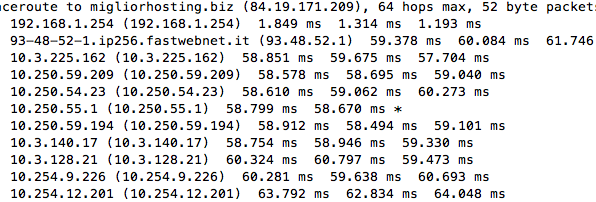
\includegraphics[scale=1]{img/083.png}
		\caption{Esempio di traceroute}
		\label{fig: 083}
	\end{center} 
\end{figure}
\subsubsection{Riassunto del calcolo dei ritardi}
\begin{itemize}
	\item \textbf{Ritardo di propagazione}: $\dfrac{d}{v}$ dove d è la distanza tra due router e v la velocità di propagazione del mezzo (m/s)
	\item \textbf{Ritardo di trasmissione}: $\dfrac{L}{R}$ dove L è la grandezza del pacchetto e R la velocità di trasmissione del link (bit/s)
\end{itemize}

\subsection{Strati protocollari}
\subsubsection{Architettura stratificata}
Per ridurre la complessità progettuale, i progettisti della rete organizzano i protocolli a strati (layer) o livelli.

Con un'architettura a strati dei protocolli, ciascun controllo appartiene a uno degli strati. Ciascun protocollo appartiene a uno degli strati, quindi il protocollo nello strato specifico è condiviso tra tutte le entità della rete che condividono quel protocollo. Queste entità comunicano tra di loro scambiandosi i messaggi dello strato n. Questi messaggi sono chiamati \textbf{n-PDU (layer-n Protocol Data Units)}. Il formato di una n-PDU è definito dal protocollo dello strato n. Quando presi nel loro insieme, i protocolli dei bari strati sono chiamati \textbf{pila protocollare}.

Un concetto chiave è quello di \textbf{modello di servizio} di uno strato: si dice che lo strato $$n - 1$$ offre servizi allo strato n.
\paragraph{Funzione degli strati}
Ciascuno strato può eseguire uno o più di questi compiti:
\begin{itemize}
	\item Controllo dell’errore
	\item Controllo del flusso
	\item Frammentazione e riassemblaggio
	\item Multiplexing
	\item Instaurazione della connessione
\end{itemize}
\subsubsection{La pila protocollare di internet}
È costituita da cinque strati

\begin{figure}
	\begin{center}
		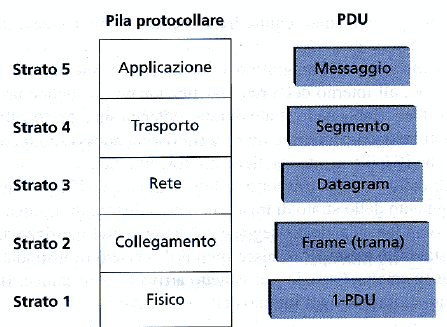
\includegraphics[scale=1]{img/008.png}
		\caption{Protocollo a strati, livello = PDU}
	\end{center} 
\end{figure}
Ad ogni livello corrisponde un tipo di pacchetto di informazione:
\begin{itemize}
	\item Livello di applicazione: messaggio
	\item Livello di trasporto: segmenti
	\item Livello di rete: datragrammi
	\item Livello di collegamento: frame
\end{itemize}
\paragraph{Strato di applicazione}
È responsabile del supporto delle applicazioni della rete, comprende molti protocolli tra i quali http, SMTP e FTP.
\paragraph{Strato di trasporto}
Vi risiedono i due protocolli, TCP e UDP:
\begin{itemize}
	\item TCP è un servizio orientato alla connessione con garanzia di consegna e un controllo di flusso (ovvero di adattamento tra la velocità del mittente e del destinatario)
	\item UDP fornisce un servizio senza connessione per applicazioni che possono accettare una perdita di pacchetti (ad esempio uno stream video)
\end{itemize}
\paragraph{Strato di rete}
È responsabile dell'instradamento dei datagram da un host all'altro. Contiene il protocollo IP, utilizzato da tutti i componenti di internet che hanno uno strato di rete. \\
I protocolli dello strato di trasporto (TCP e UDP) in un host sorgente passano un segmento dello strato di trasporto e un indirizzo di destinazione allo strato IP.
\paragraph{Strato di collegamento}
Per muovere un pacchetto da un nodo al successivo sul percorso, lo strato di rete deve delegare il servizio allo strato di collegamento. In particolare, a ciascun nodo IP passa il datagram allo strato di collegamento, che lo invia al nodo successivo lungo il percorso.
\paragraph{Strato fisico}
Il suo compito è quello di muovere singoli bit all'interno della rete da un nodo all'altro.

\subsubsection{Incapsulamento}
Ogni livello incapsula il messaggio dello strato superiore, questo vuol dire che il messaggio dello strato superiore diventa le informazioni di quello successivo.
\pagebreak

\section{Livello di trasporto}
\subsection{Introduzione e servizio dello strato di trasporto}
Un protocollo dello strato di trasporto fornisce una commutazione logica fra i processi applicativi che funzionano su host differenti. Per comunicazione logica intendiamo che dal punto di vista dell'applicazione, è come se i terminali su cui girano i processi fossero direttamente connessi. I processi applicativi usano la comunicazione logica fornita dallo strato di trasporto per scambiarsi messaggi, senza doversi occupare dei dettagli dell'infrastruttura fisica usata per trasportarli.\\ \\
\textbf{Attenzione}: i protocolli dello strato di trasporto sono implementati nei terminali ma non nei router della rete. \\ \\
\begin{figure}
	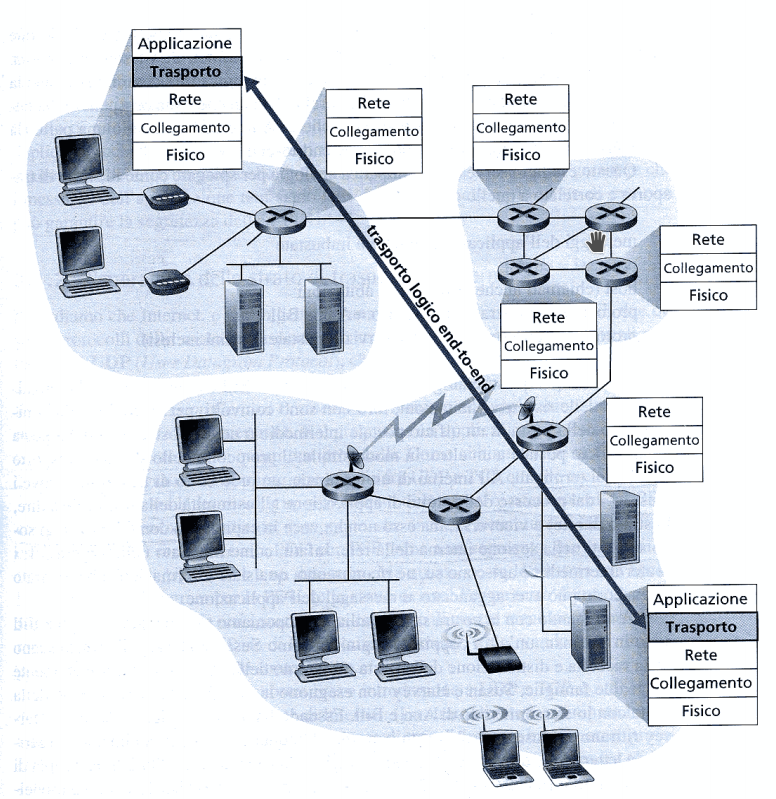
\includegraphics[scale=0.6]{img/009.png}
	\caption{Lo strato di trasporto fornisce una comunicazione logica piuttosto che fisica tra le applicazioni}
\end{figure}
\subsubsection{Relazione fra gli strati di trasporto e di rete}
Mentre un protocollo dello strato di trasporto fornisce una \emph{comunicazione logica tra i processi} che funzionano su differenti host, un protocollo dello strato di rete fornisce la \emph{comunicazione logica fra gli host}.
\subsubsection{Panoramica dello strato di trasporto in internet}
Per semplificare la terminologia, nel contesto di internet, ci riferiamo alla 4-PDU come a un segmento. \\ \\
\textbf{Attenzione}: nella letteratura ci si riferisce alla PDU per TCP come a un segmento, al PDU per UDP come a un datagram. In questo testo, però, si utilizzerà solo la notazione "segmento".\\ \\
Il protocollo dello strato di rete ha un nome: \textbf{IP} (Internet Protocol). L'IP fornisce la comunicazione logica fra gli host. Il modello di servizio di IP è un \textbf{servizio best effort}, ovvero che "fa del suo meglio" per consegnare i segmenti fra i due host ma senza garanzie; per questo motivo IP è un \textbf{servizio inaffidabile}. Ricordiamo che \textbf{ciascun host ha un unico indirizzo IP}.\\
La maggior responsabilità di UDP e TCP è di estendere il servizio di spedizione di IP tra due terminali al servizio di spedizione fra due processi che funzionano sui terminali. L'estensione della spedizione da host a host alla spedizione da processo a processo è detta \textbf{multiplexing} e \textbf{demultiplexing} dello strato di trasporto. UDP e TCP forniscono anche un controllo dell'integrità inserendo campi di rilevamento di errori nelle loro intestazioni. \\
Questi due servizi, \textbf{spedizioni di dati da processo a processo} e \textbf{verifica degli errori} sono i due soli servizi forniti da UDP, infatti UDP è un servizio inaffidabile.\\
TCP offre molti servizi addizionali; prima di tutto un \textbf{trasferimento affidabile dei dati} usando controllo del flusso, numeri di sequenza, riscontri (acknowledgment) e timer, in questo modo TCP si assicura che i dati siano spediti da un processo mittente al destinatario correttamente e in ordine. TCP converte perciò il servizio inaffidabile IP in un servizio affidabile. \\*
TCP usa anche il controllo di congestione, ovvero previene la saturazione da parte di qualsiasi connessione TCP della rete suddividendo equamente la banda di un link congestionato tra le connessioni TCP che lo attraversano. I campi dei numeri di porta sorgente e destinazione in un segmento dello strato di trasportosano. Il traffico UDP, invece, non è regolabile.
\subsection{Multiplexing e demultiplexing}
Per l'host destinatario, lo strato di trasporto riceve i segmenti (le PDU dello strato di trasporto) allo strato di rete posto subito sotto di esso. Lo strato di trasporto ha la responsabilità di inviare i dati di questi segmenti all'appropriato processo applicativo che funziona sull'host.
Per comprendere come funzioni ricordiamoci prima di tutto che un processo ha un \textbf{socket}, che è una porta attraverso la quale i dati passano dalla rete al processo, e attraverso la quale i dati passano dal processo alla rete. Lo strato di trasporto nel terminale ricevente non consegna effettivamente i dati direttamente a un processo, \textbf{ma li consegna invece a un socket intermediario}. Possono esserci più socket e tutte hanno un identificatore unico. L'identificatore dipende dal fatto che il socket sia UDP o TCP.\\
Ogni segmento dello strato di trasporto ha un insieme di campi dedicati all'identificazione del socket; lo strato di trasporto esamina questi capi per determinare il socket ricevente e indirizzargli i segmenti.
Il lavoro di recapitare i dati in un segmento allo strato di trasporto corretto socket è chiamato \textbf{demultiplexing}. Il lavoro di ottenere i dati dall'host sorgente dai diversi socket, completare i dati con le informazioni di intestazione (usate durante il demultiplexing) per creare segmenti, e di passare i segmenti allo strato di rete è detto \textbf{multiplexing}.
\begin{figure}
	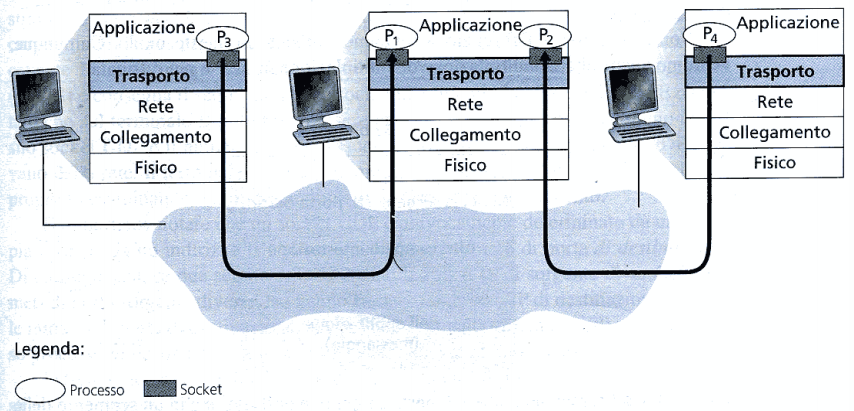
\includegraphics[scale=0.6]{img/010.png}
	\caption{Multiplexing e demultiplexing dello strato di trasporto}
\end{figure}
Ogni segmento ha dei campi speciali che indicano il socket al quale il segmento deve essere consegnato. Questi campi speciali sono \textbf{il campo numero di porta sorgente}	e \textbf{il campo numero di porta di destinazione}. Ciascun numero di prota è a \textbf{16 bit (0-65535}. I numeri di porta che vanno da 0 a 1023 sono chiamati \textbf{numeri di porta ben conosciuti} e sono riservati, il che significa che sono dedicati per l'uso con protocolli applicativi noti come HTTP (80), FTP (21). L'elenco dei numeri di porta ben conosciuti è fornito nella RFC 1700.\\
Quando progettiamo una nuova applicazione dobbiamo assegnare un numero di porta. \\
Questo è il funzionamento di UDP, mentre TCP sfrutta sistemi più raffinati. \\
Un socket UDP è univocamente determinato da una coppia formata da un indirizzo IP di destinazione e un numero di porta di destinazione.


\begin{figure}
	\begin{center}
		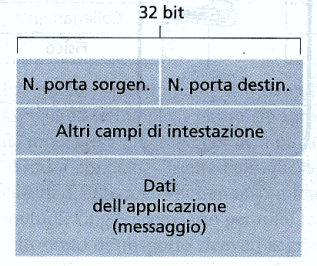
\includegraphics[scale=1]{img/011.png}
		\caption{I campi dei numeri di porta sorgente e destinazione in un segmento dello strato di trasporto} 
	\end{center}
	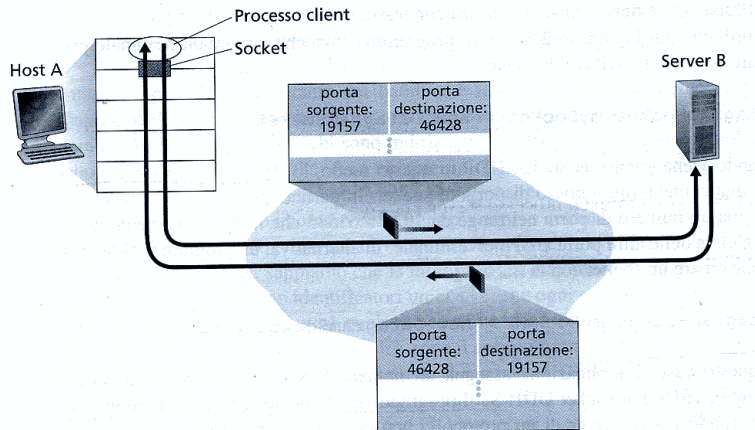
\includegraphics[scale=0.6]{img/012.png}
	\caption{L'inversione dei numeri di porta sorgente e destinazione}
\end{figure}


\subsubsection{Multiplazione e demultiplazione orientate alla connesione}
Una sottile differenza tra un socket TCP e un socket UDP è che un socket TCP è identificato da una 4-upla:
\begin{itemize}
	\item indirizzo IP di sorgente
	\item numero di porta sorgente
	\item indirizzo IP di destinazione
	\item numero di porta di destinazione
\end{itemize}
In particolare, e al contrario di UDP, due segmenti TCP entranti che recano indirizzi IP di sorgente diversi o numeri di porta sorgente diversi saranno diretti verso due diversi socket. \\

\subsection{Trasporto senza connessione: UDP}
L'UDP, definito nella RFC 768, esegue il minimo che un protocollo di trasporto può fare. Tranne che per la funzione di multiplexing/demultiplexing e qualche piccola verifica degli errori, esso aggiunge poco all'IP. Semplicemente aggiunge i numeri di porta di origine e destinazione, poi lo strato di rete incapsula i segmenti in un datagram IP e quindi poi li invia all'host di destinazione in modalità best effort. \\ \\
\textbf{Attenzione}: con l'UDP, prima della spedizione del segmento, \textbf{non c'è handshake} fra le entità dello strato di trasporto che spediscono e ricevono. Per questo si dice che l'UDP è senza connessione. \\ \\
Il DNS è un esempio di un protocollo dello strato di applicazione che usa l'UDP: quando l'applicazione DNS in un host vuole fare una richiesta, essa costruisce un messaggio di richiesta DNS e passa il messaggio a UDP. Infatti, se non riceve risposta, essa tenta ancora di inviare la richiesta a un altro server dei nomi, o informa l'applicazione che ha fatto la richiesta che gli è impossibile ottenere una risposta. \\
Perchè scegliere UDP? Per i seguenti motivi:
\begin{itemize}
	\item \textbf{non viene creata alcuna connessione}: UDP non introduce alcun ritardo dovuto alla fase di impostazione della connessione (handshake)
	\item \textbf{nessuno stato della connessione}: l'UDP non mantiene lo stato della connessione e non ha traccia dei parametri di controllo della congestione e dei numeri di sequenza e riscontro, per questo un server può supportare molti più client attivi quando l'applicazione funziona su UDP invece che su TCP
	\item \textbf{Poco sovraccarico \textit{(overhead)} dovuto all'intestazione del pacchetto}: il segmento TCP ha overhead di 20 byte per segmento, UDP solo 8
	\item \textbf{Controllo di livello applicativo più fine su quali dati vengono mandati e quando}: UDP, appena un processo applicativo manda dati a UDP, li impacchetta all'interno di un segmento e passa immediatamente il segmento allo strato di rete. TCP, invece, "strozza" il mittente quando uno o più link tra i terminali di sorgente e destinazione diventano eccessivamente congestionati. Inoltre TCP continua a rimandare un segmento fino a che non riceve l'acknowledgment, rallentando quindi la comunicazione
\end{itemize}
\begin{figure}
	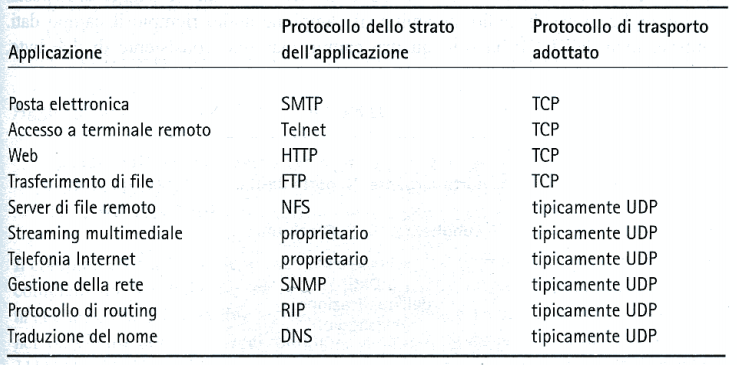
\includegraphics[scale=0.6]{img/014.png}
	\caption{Applicazioni diffuse in internet e protocolli che adottano}
\end{figure}
\textbf{Attenzione}: UDP può essere usato per generare un servizio affidabile, semplicemente i controlli di riscontro e ritrasmissione devono essere inseriti nell'applicazione stessa, cosa tediosa ma molto vantaggiosa per velocità di comunicazione e funzionalità. Molte applicazioni streaming sfruttano questo sistema. \\
\subsubsection{Struttura del segmento UDP}

\begin{figure}
	\begin{center}
		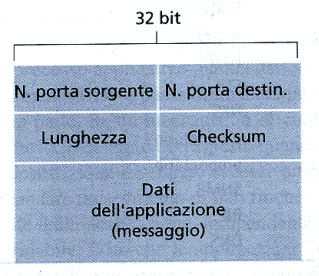
\includegraphics[scale=1]{img/015.png}
		\caption{Struttura del segmento UDP}
	\end{center}
\end{figure}

La \textbf{checksum} \textit{(somma di controllo)} è usata dall'host ricevente per controllare se sono stati introdotti errori nel segmento.
\subsubsection{Checksum di UDP}
La checksum di UDP effettua il rilevamento degli errori, ovvero se i bit del segmento sono stati alterati nel loro percorso. \\
\begin{itemize}
	\item \textbf{Lato mittente}: si effettua il complemento a 1\footnote{Si ottiene convertendo tutti gli 0 in 1 e tutti gli 1 in 0} della somma di tutte le parole a 16 bit del segmento, scartando ogni overflow. Il risultato è inserito nel campo checksum del segmento UDP.
	\item \textbf{Lato ricevente}: riceve tutte le parole a 16 bit, inclusa la checksum. se nel pacchetto non sono stati introdotti errori, la somma al ricevente deve essere 1111111111111111. \\
\end{itemize}
Alcune implementazioni dell'UDP scartano semplicemente il segmento danneggiato, altri lo passano all'applicazione con l'aggiunta di un'avvertenza.

\subsection{Principi di un trasferimento affidabile dei dati}
\begin{figure}
	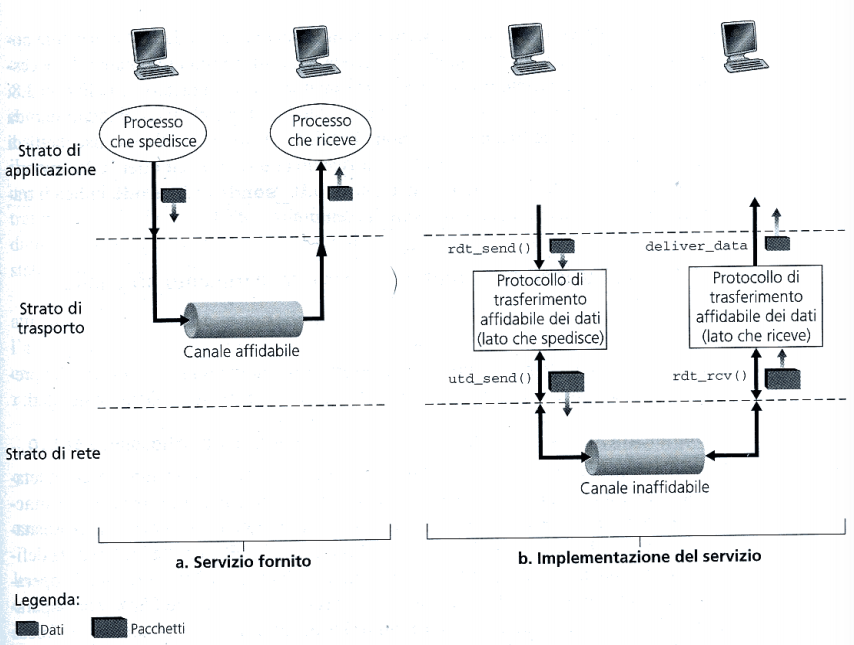
\includegraphics[scale=0.6]{img/016.png}
	\caption{Astrazione di un servizio affidabile. rdt = reliable data trasfer, udt = unreliable data trasfer}
\end{figure}
È compito del protocollo di \textbf{trasferimento affidabile dei dati} l'implementazione di quest'astrazione del servizio. La difficoltà di questo compito deriva dal fatto che lo strato sottostante il protocollo di trasferimento affidabile dei dati può essere inaffidabile. Ad esempio, TCP è un protocollo di trasferimento affidabile che è implementato sopra uno strato di rete (IP) inaffidabile da terminale a terminale. \\
Per questa trattazione assumeremo che lo strato di rete sia inaffidabile. Tratteremo, inoltre, solo il caso di trasferimento unidirezionale dei dati. Il caso bidirezionale \textit{(full duplex} dei dati non è più complicato ma è più noioso da spiegare. \\
\subsubsection{Costruzione di un protocollo per il trasferimento affidabile dei dati}
Ora analizzeremo una serie di protocolli di complessità crescente fino ad un perfetto protocollo di trasferimento affidabile dei dati.
\paragraph{Trasferimento affidabile dei dati su un canale completamente affidabile: rdt1.0}
\begin{figure}
	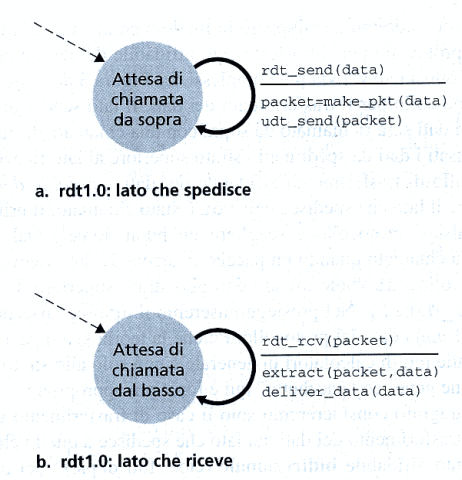
\includegraphics[scale=0.6]{img/017.png}
	\caption{Macchine a stati finiti \textit{rdt1.0: un protocollo per un canale completamente affidabile (FSM - Finite State Machine}}
\end{figure}
Consideriamo il caso in cui il canale sottostante sia completamente affidabile.
Le frecce delle due FSM\footnote{Per comprendere completamente il funzionamento di una FSM leggere gli appunti di Linguaggi e computabilità} indicano il passaggio del protocollo da uno stato all'altro. Gli eventi che causano la transizione sono illustrati sopra la linea orizzontale e l'azione/i intraprese sono illustrate sotto la linea. Quando non si verifica alcun evento o non si effettua un'azione si usa il simbolo $\lambda$ (lambda). Lo stato iniziale è simboleggiato dalla freccia tratteggiata. \\
\begin{itemize}
	\item \textbf{Lato mittente}: quando si ricevono i dati vengono inseriti in un pacchetto e viene spedito
	\item \textbf{Lato ricevente}: quando viene ricevuto un pacchetto vengono estratti i dati e vengono inviati allo strato superiore
\end{itemize}
Con un canale completamente affidabile non serve alcun feedback da inviare al mittente.

\paragraph{Trasferimento affidabile dei dati su un canale con errori sui bit: rdt2.0} \label{par: numSequenza}
\begin{figure}
	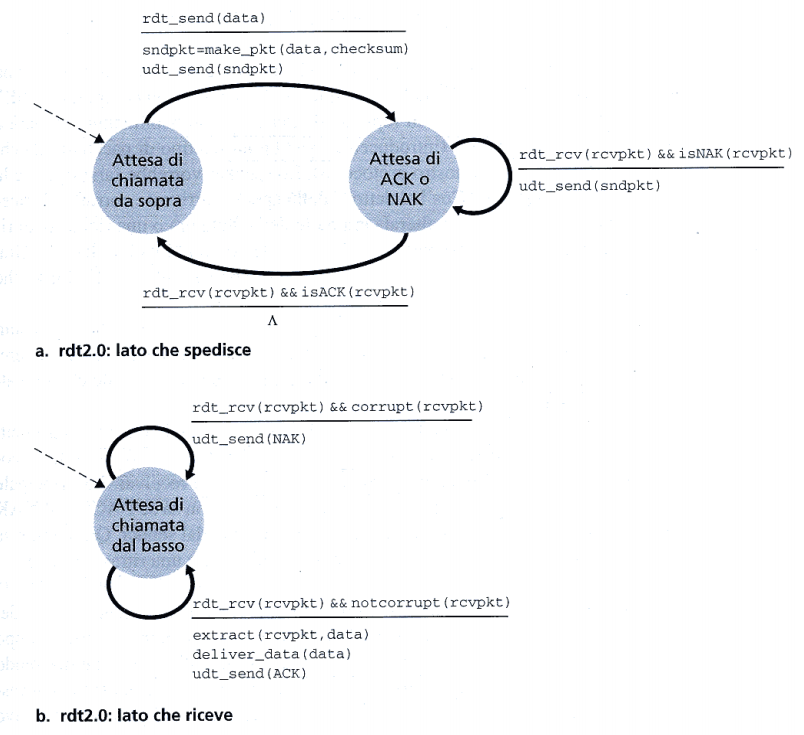
\includegraphics[scale=0.6]{img/018.png}
	\caption{rdt2.0: un protocollo per un canale con errori sui bit}
\end{figure}
Ora inseriamo la possibilità che i pacchetti possano essere alterati. Per ora assumiamo che tutti i pacchetti siano ricevuti.\\
I protocolli per il trasferimento affidabile dei dati che si basano sulle ritrasmissioni sono conosciuti come \textbf{protocolli ARQ (Automatic Repeat reQuest}. Fondamentalmente, in questi protocolli sono richieste tre funzionalità addizionali:
\begin{itemize}
	\item \textbf{Rilevamento degli errori}
	\item \textbf{Feedback dal ricevente}: il ricevente invia un feedback esplicito al mittente,  riscontri positivi \textbf{(ACK, positive acknowledgement)} e riscontri negativi \textbf{(NAK, Negative acknowledgement)}
	\item \textbf{Ritrasmissione}: un pacchetto che arriva con errori al ricevente sarà ritrasmesso dal mittente
\end{itemize}
Ora, vedendo la figura, notiamo che il mittente ha due stati, ovvero dopo aver spedito il pacchetto attende di ricevere l'ACK o il NAK. Se viene restituito un ACK, il mittente sa che il pacchetto più recente è stato ricevuto e allora il protocollo ritorna nello stato di attesa dei dati dallo strato superiore. Se riceve un NAK, allora ritrasmette l'ultimo pacchetto e attende un altro ACK o un NAK. \\
È importante notare che quando il mittente è nello stato di attesa di ACK o NAK non può accettare altri dati dallo strato superiore. Questo tipo di protocollo è conosciuto come \textbf{protocollo stop-and-wait \textit{(fermati e aspetta)}}. \\
Il lato ricevente ha ancora un singolo stato, semplicemente invierà un ACK o un NAK in base allo stato del pacchetto. \\
Ora, rimane un problema: i pacchetti ACK e NAK potrebbero essere alterati a loro volta. Come risolvere? Ci sono due possibilità:
\begin{itemize}
	\item Aggiungere un numero di bit alla checksum sufficiente a permettere al ricevente non solo di rilevare, ma anche di correggere, eventuali errori dei bit.
	\item Il mittente può semplicemente reinviare i pacchetti quando riceve un pacchetto ACK o NAK difettoso. Questo modo introduce duplicati dei pacchetti. Il problema è che se il ricevente non sa se l'ACK o il NAK che ha inviato per ultimo è stato ricevuto correttamente dal mittente. Quindi non sa a priori se il pacchetto è nuovo o è una ritrasmissione.
\end{itemize}
Una semplice soluzione a questo problema è aggiungere un nuovo campo ai pacchetti dati: \textbf{un numero di sequenza} che il ricevente può semplicemente controllare per determinare se il pacchetto è nuovo o ritrasmesso. \\
Poichè abbiamo assunto che il canale non possa perdere pacchetti, i pacchetti non hanno bisogno di indicare a loro volta il numero di sequenza. Ora le FSM di mittente e ricevente hanno numero doppio degli stati rispetto a prima, questo perchè lo stato del protocollo deve adesso tenere in conto se il pacchetto attualmente in fase di spedizione o di ricezione dovrà avere numero di sequenza 0 o 1. \pagebreak

\begin{figure}
		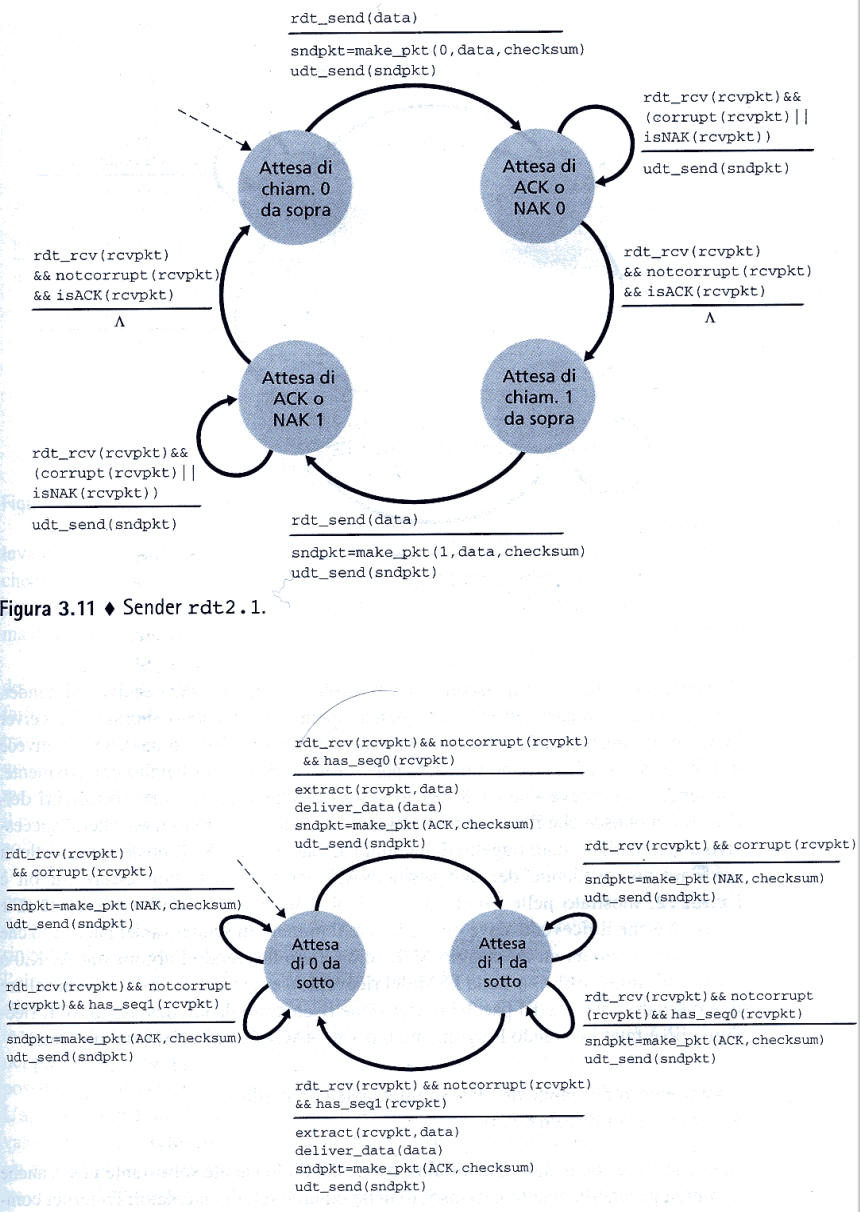
\includegraphics[scale=0.6]{img/019.png}
		\caption{Sender e reciver 2.0}
\end{figure}
\pagebreak

\begin{figure}
		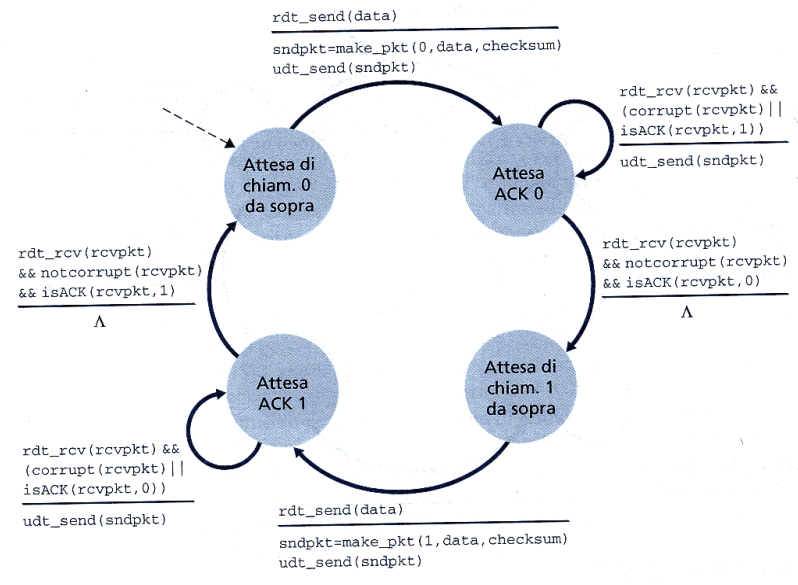
\includegraphics[scale=0.6]{img/020.png}
		\caption{Sender 2.2}
\end{figure}
Il protocollo rdt2.1 usa ACK e NAK dal ricevente al mittente. Quando riceve un pacchetto fuori sequenza o alterato inviai un NAK. Possiamo ottenere lo stesso effetto di un NAK se viene inviato ogni volta un ACK col numero dell'ultimo pacchetto ricevuto correttamente. Un mittente che riceve due ACK con lo stesso numero di sequenza (ovvero \textbf{duplicati dell'ACK}) capisce che l'ultimo pacchetto non è andato a buon fine. \\
rdt2.2 introduce questa modifica, eliminando il NAK.

\paragraph{Traferimento affidabile dei dati su un canale con perdite e con errori sui bit: rdt3.0}
\begin{figure}
	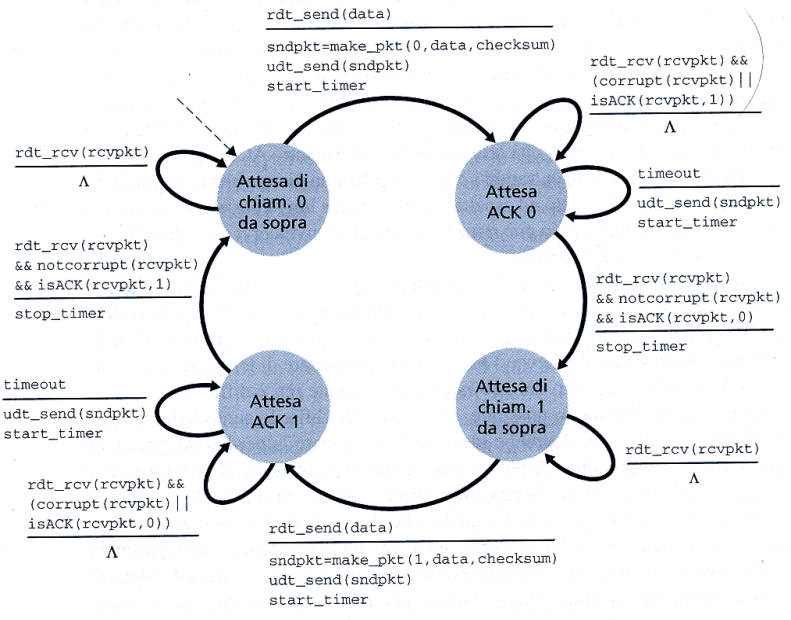
\includegraphics[scale=0.6]{img/021.png}
	\caption{Sender rdt3.0}
\end{figure}
Supponiamo ora che il canale possa anche perdere i pacchetti, evento non raro. In questo caso ci sono due nuovi problemi:
\begin{itemize}
	\item rilevare la perdita dei pacchetti
	\item cosa fare quando si perdono i pacchetti
\end{itemize}
L'uso di checksum, numeri di sequenza, pacchetti ACK e ritrasmissione ci permettono di risolvere l'ultima difficoltà, per la prima invece dobbiamo sviluppare nuovi sistemi. \\
Supponiamo che il mittente trasmetta un pacchetto di dati o che il ricevente invii un pacchetto o un riscontro e questi vengano persi. In entrambi i casi il mittente non riceve mai un riscontro. Se è disposto ad attendere abbastanza per essere sicuro che il pacchetto sia stato perso, allora può rispedirlo. La domanda ora è: per quanto deve attendere? \\
Il primo fattore è includere almeno un tempo equivalente al ritardo per un percorso circolare tra mittente e destinatario (che potrebbe comprendere il buffering ai router intermedi o ai gateway), più un certo ammontare di tempo richiesto dall'elaborazione di un pacchetto dal lato ricevente. La difficoltà nel definire questo ritardo porta l'eventualità della presenza di duplicati di pacchetti dati nel canale di comunicazione. rdt2.2 ha già introdotto sufficienti strumenti per la gestione dei duplicati. \\
Per implementare un meccanismo di ritrasmissione basato sul tempo, è necessario un \textbf{meccanismo di conto alla rovescia \textit{(countdown timer)}} che possa interrompere il mittente dopo che è trascorso un certo tempo. Quindi, il mittente dovrà:
\begin{itemize}
	\item avviare il timer ogni volta che un pacchetto viene spedito
	\item rispondere alle interruzioni del timer
	\item arrestare il timer
\end{itemize}
Ora, come può il mittente capire se l'ACK ricevuto riguarda l'ultimo pacchetto o un altro? Introducendo nel pacchetto di ACK un \textbf{campo di riscontro \textit{acknowledgement field)}} che conterrà il numero di sequenza del pacchetto dati al quale corrisponde l'ACK.
Come illustrato nella figura, poiché i numeri di sequenza si alternano tra 0 e 1, il protocollo edt3.0 qualche volta è detto \textbf{protocollo a bit alternati \textit{(alternating-bit protocol)}}. \\ \\
Abbiamo assemblato un protocollo di trasferimento dei dati: checksum, numeri di sequenza, timer, ACK e NAK. Abbiamo ora un protocollo per il trasferimento affidabile dei dati che funziona!
\begin{figure}
	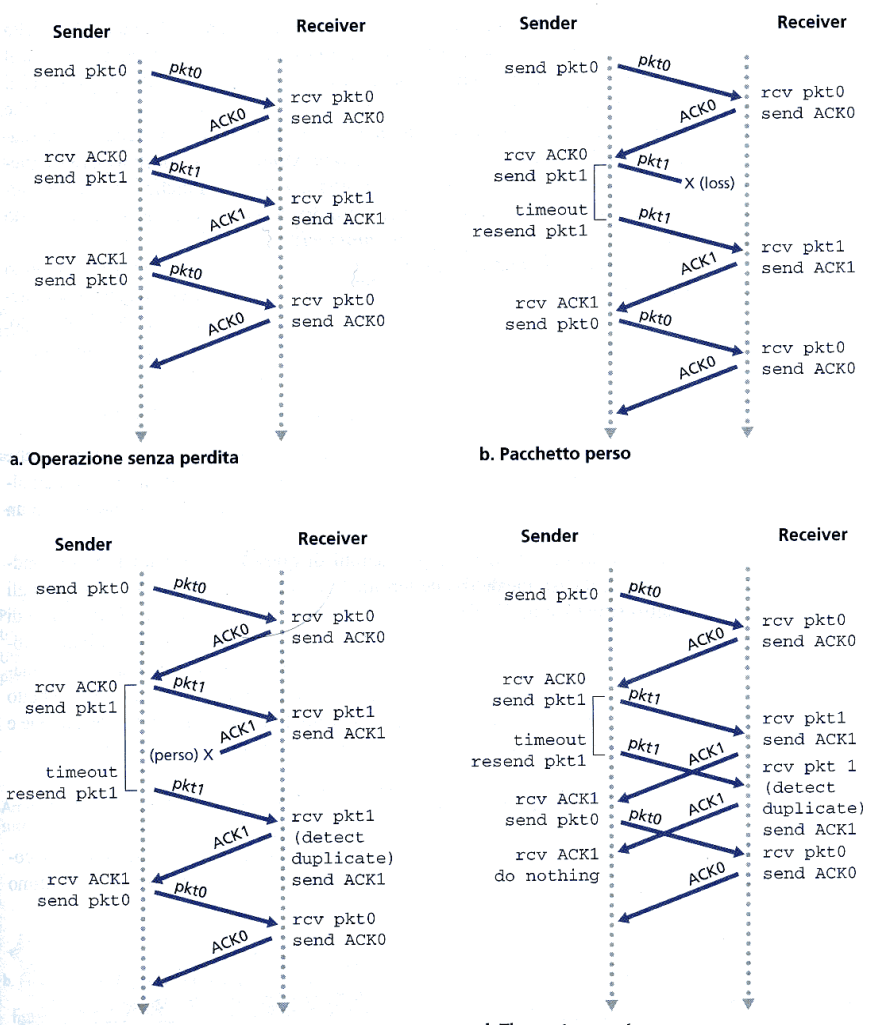
\includegraphics[scale=0.6]{img/022.png}
	\caption{Operazioni dell'rdt3.0, il protocollo a bit alternati}
\end{figure}
\subsubsection{Protocolli pipeline per il trasferimento affidabile dei dati}
Il problema principale di rdt3.0 è il fatto che è un protocollo stop-and-wait. Infatti, in un protocollo stop-and-wait il mittente è spesso in attesa (idle) poichè deve aspettare una risposta dal ricevente. Un modo per risolvere le attese troppo lunghe è permettere al mittente di inviare più pacchetti senza aspettare i riscontri. Questa tecnica è detta \textbf{pipelining}. Il pipelining ha molte conseguenze per i protocolli con trasferimento affidabile dei dati:
\begin{itemize}
	\item La gamma dei numeri di sequenza deve essere aumentata per evitare ripetizioni
	\item i due host devono poter memorizzare più di un pacchetto.
\end{itemize}
la gamma di numeri di sequenza richiesti e i requisiti di buffering dipendono dal modo in cui il protocollo di trasferimento dei dati risponde alle perdite, all'alterazione e all'eccessivo ritardo dei pacchetti.
\begin{figure}
	\begin{center}
		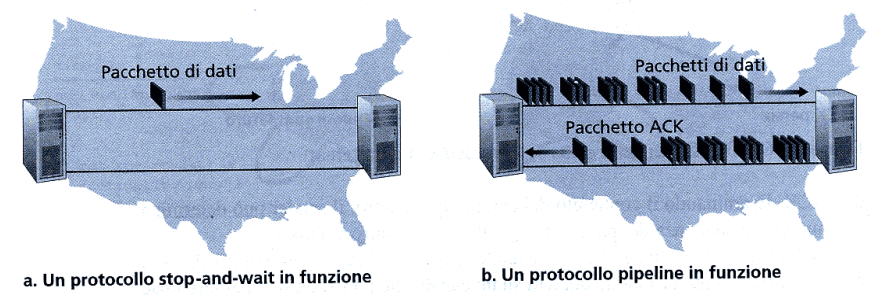
\includegraphics[scale=0.6]{img/023.png}
		\caption{Confronto fra protocolli stop-and-wait e pipeline}
		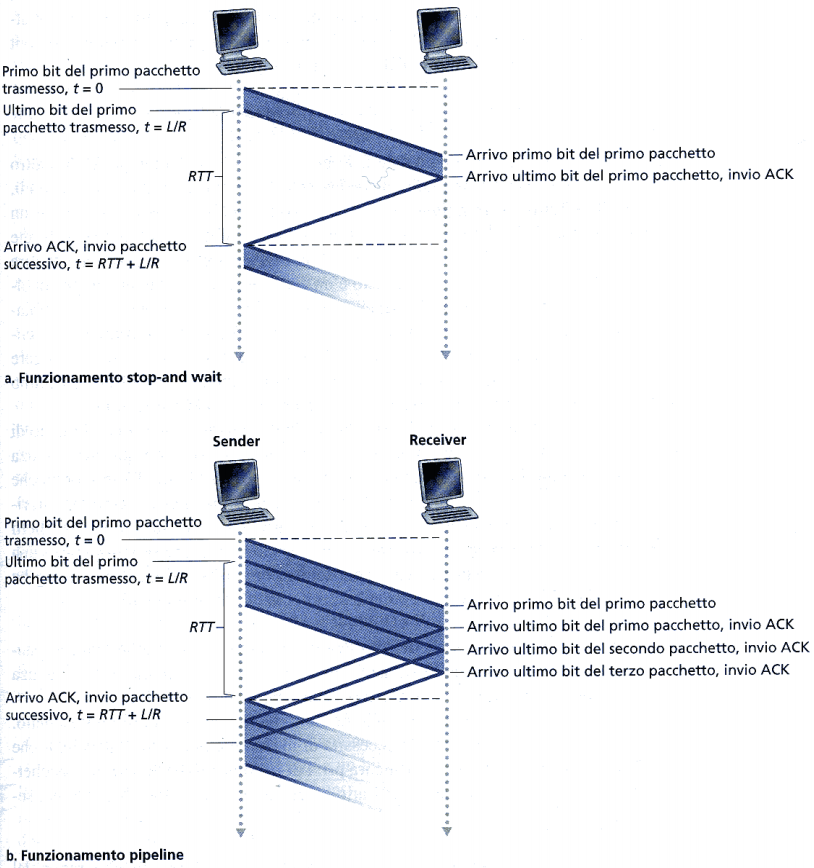
\includegraphics[scale=0.6]{img/024.png}
		\caption{Spedizione stop-and-wait e pipeline}
	\end{center}
\end{figure}
Si possono identificare due approcci alla riparazione degli errori:
\begin{itemize}
	\item Go-Back-n
	\item ripetizione selettiva
\end{itemize}
\subsubsection{Go-Back-N (GBN)}
Il mittente può trasmettere pacchetti multipli senza aspettare il riscontro, ma è costretto ad avere non più di un certo numero massimo consentito di pacchetti non riscontrati, N, nella pipeline.
\begin{figure}
	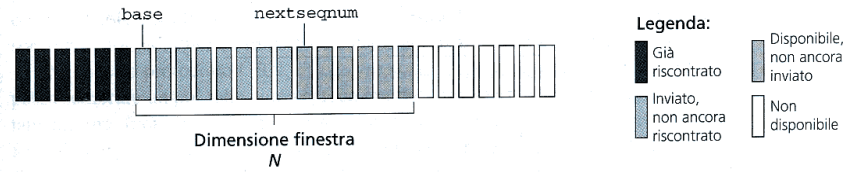
\includegraphics[scale=0.6]{img/025.png}
	\caption{Il punto di vista del sender sui numeri di sequenza nel GBN}
\end{figure}
Se definiamo come \emph{base} il numero di sequenza del paccehtto più vecchio senza riscontro e come \emph{nextseqnum} il più piccolo numero di sequenza inutilizzato, allora nella gamma dei numeri di sequenza si possono identificare quattro intervalli:
\begin{itemize}
	\item \emph{[0, base-1]}: pacchetti già trasmessi
	\item \emph{[base, nextseqnum-1]}: pacchetti che sono stati spediti e ancora senza riscontro
	\item \emph{[nextseqnum, base+N-1]}: questi numeri di sequenza nell'intervallo possono essere usati per i pacchetti che possono essere spediti immediatamente
	\item \emph{>base+N}: non possono essere usati finchè un pacchetto non riscontrato viene riscontrato
\end{itemize}
N è noto come \textbf{dimensione della finestra} e il protocollo GBN come \textbf{protocollo a finestra scorrevole}.
\begin{figure}
	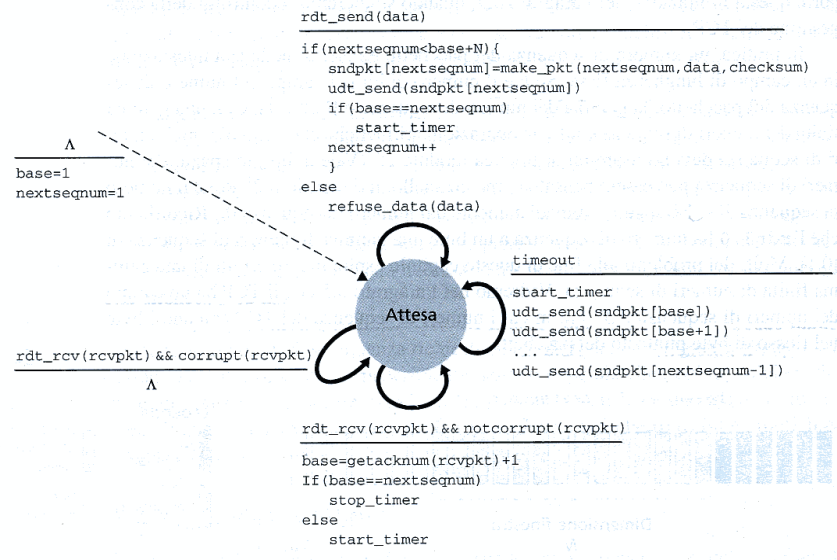
\includegraphics[scale=0.6]{img/026.png}
	\caption{Descrizione dell'FSM estesa del sender GBN}
\end{figure}
Il sender GBN deve affrontare tre tipi di eventi:
\begin{itemize}
	\item Chiamata da sopra: quando $rdt_send()$ è chiamata da sopra, il mittente prima controlla per valutare se la finestra è satura (N pacchetti in circolazione non riscontrati) e decide se spedire il nuovo pacchetto o se ritornare i dati allo strato superiore.
	\item ricezione di un ACK: un riscontro con numero di sequenza n sarà interpretato come un riscontro cumulativo che indica che tutti i pacchetti con un numero di sequenza fino a n, n compreso, sono stati correttamente ricevuti
	\item un evento timeout: se interviene un timeout, il mittente rispedisce \emph{tutti} i pacchetti che sono già stati spediti ma che non hanno ricevuto riscontro
\end{itemize}
\begin{figure}
	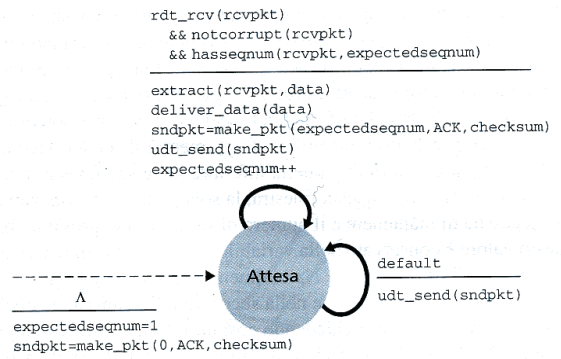
\includegraphics[scale=0.6]{img/027.png}
	\caption{Descrizione dell'FSM estesa del receiver GBN}
\end{figure}
Le azioni del ricevente sono anch'esse semplici. Se un pacchetto con un numero di sequenza n è ricevuto correttamente ed è in ordine (ovvero se l'ultimo pacchetto inoltrato allo strato superiore è l'n*1) il ricevente invia un ACK per il pacchetto n. Negli altri casi il pacchetto viene scartato e rispedisce un ACK per l'ultimo pacchetto in ordine. In questo protocollo GBN, il ricevente scarta i pacchetti non in ordine, questo permette di non dover mantenere in memoria alcun pacchetto fuori ordine. Ovviamente lo svantaggio è la richiesta di più ritrasmissioni eventuali.
\subsubsection{Ripetizione selettiva (SR)}
Esistono casi nei quali GBN può avere problemi di prestazioni, ad esempio quando la dimensione della finestra e il prodotto ritardo-larghezza di banda sono entrambi grandi, nelle pipeline possono trovarsi molti pacchetti. Un singolo errore può costringere GBN a ritrasmettere un grande numero di pacchetti, magari non tutti necessari. In più queste ritrasmissioni possono saturare la pipeline. \\
I protocolli a ripetizione selettiva evitano le ritrasmissioni non necessarie grazie alla rispedizione di quei soli pacchetti che si sospetta siano giunti al ricevente con errori. Una finestra di dimensioni N dovrà ancora essere usata per limitare il numero di pacchetti da evadere, non riscontrati, nella pipeline.
\begin{figure}
	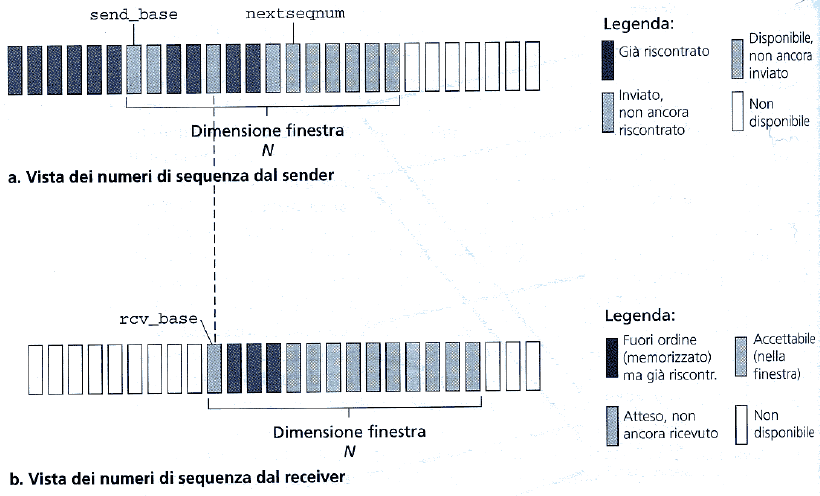
\includegraphics[scale=0.6]{img/028.png}
	\caption{SR: viste degli intervalli dei numeri di sequenza dal sender e dal receiver}
	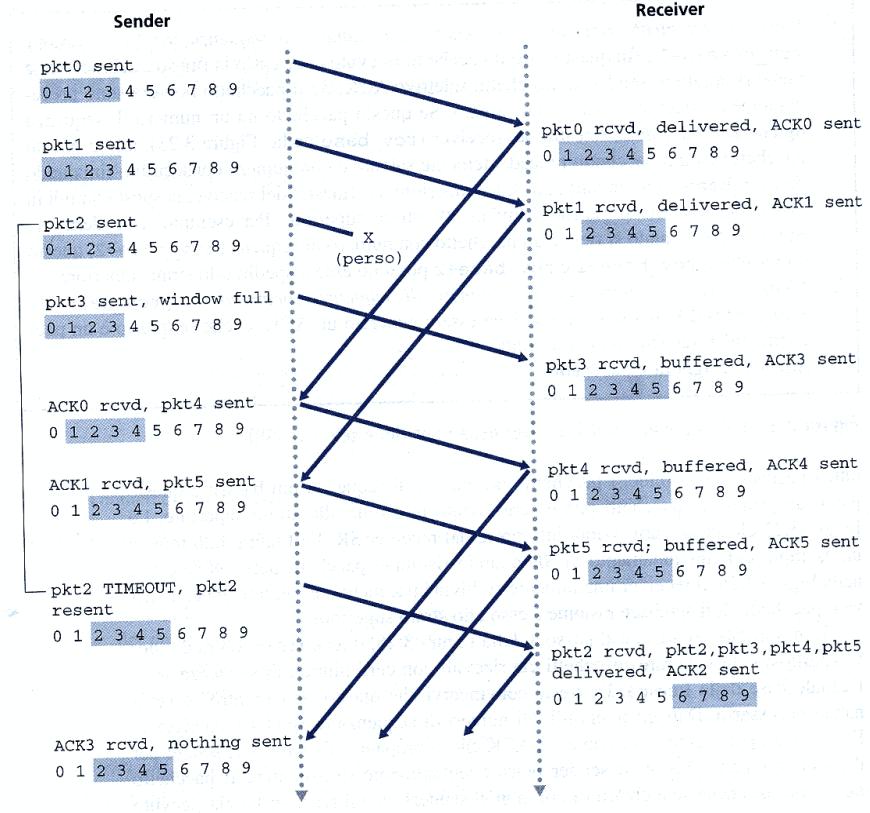
\includegraphics[scale=0.6]{img/029.png}
	\caption{Operazioni del SR}
\end{figure}
Il problema è identificare la dimensione necessaria della finestra affinché non ci siano errori.
\pagebreak

\subsection{Trasporto orientato alla connessione: TCP}
\subsubsection{La connessione TCP}
Si dice che TCP è \textbf{orientato alla connessione} perché prima che un processo applicativo possa cominciare a spedire dati, i due processi devono scambiarsi un \textbf{handshake} \textit{(stretta di mano)}, ovvero devono prima inviarsi alcuni segmenti preliminari per stabilire i parametri del successivo trasferimento di dati.
TCP funziona solo nei terminali e non negli elementi intermedi della rete, questi elementi non mantengono lo stato della connessione TCP. Infatti, i router intermedi dimenticano completamente la connessione TCP, vedono solo i datagram, non le connessioni. \\
Una connessione TCP fornisce un trasferimento dei dati \textbf{full duplex}, cioè consente ai dati di viaggiare contemporaneamente nelle due direzioni. Una connessione TCP è anche \textbf{point-to-point}, cioè fra un singolo sender e un singolo receiver. Con TCP il cosiddetto \emph{"multicasting"} (il trasferimento da un mittente a più riceventi contemporaneamente) è impossibile. \\
\textbf{Handshake a tre vie}:
\begin{itemize}
	\item il client invia uno speciale segmento TCP
	\item il server risponde con un secondo segmento speciale TCP
	\item il client risponde con un terzo segmento speciale
\end{itemize}
I primi due non contengono "carico utile" (payload), il terzo può trasportarne. \\
TCP indirizza i dati al \textbf{buffer di spedizione} (send buffer) della connessione, che è uno dei buffer che viene riservato durante l'iniziale handshake a tre vie.
\begin{figure}
	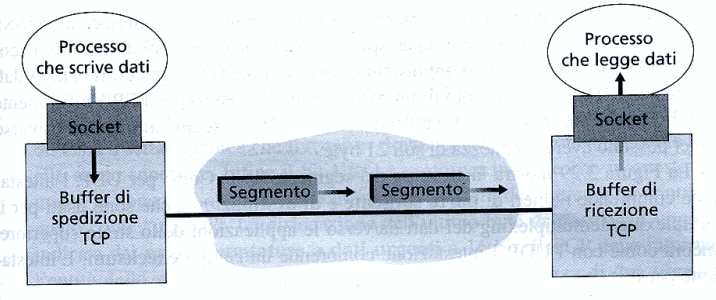
\includegraphics[scale=0.6]{img/030.png}
	\caption{Buffer di spedizione e ricezione del TCP}
\end{figure}
La quantità massima di dati che può essere prelevata e inserita in segmenti è limitata dalla \textbf{dimensione massima del segmento} (\textbf{MSS}, \textit{Maximum Segment Size}). Il valore di MSS dipende dall'implementazione del TCP (determinata dal sistema operativo) e spesso può essere configurato. \\
TCP unisce a ciascun pezzo dei dati del client un'intestazione TCP, formando così i segmenti TCP. \\
Quando il ricevente riceve i segmenti, questi sono posti nel buffer di ricezione della connessione TCP,
\subsubsection{Struttura del segmento TCP}
\begin{figure}
	\begin{center}
		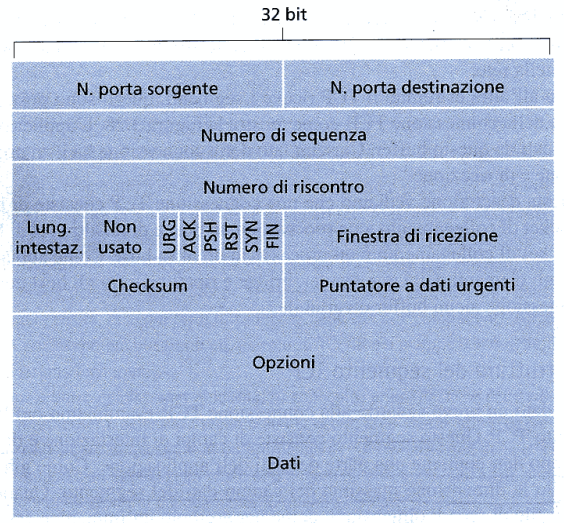
\includegraphics[scale=0.6]{img/031.png}
		\caption{Struttura del segmento TCP}
	\end{center}
\end{figure}
L'intestazione TCP è tipicamente di 20 byte. Come per UDP, l'intestazione comprende \textbf{numeri di porta sorgente e di destinazione e checksum}. Inoltre, l'intestazione TCP contiene anche:
\begin{itemize}
	\item \textbf{numero di sequenza e numero di riscontro}: 32 bit
	\item \textbf{dimensione finestra}: 16 bit
	\item \textbf{lunghezza intestazione}: 4 bit, specifica la lunghezza dell'intestazione del TCP in parole a 32 bit
	\item \textbf{opzioni}: è a lunghezza variabile, è usato quando un sender e un receiver negoziano la massima dimensione del segmento MSS o come fattore di scala della finestra per l'uso nelle reti ad alta velocità
	\item \textbf{campo flag}: 6 bit
		\begin{itemize}
			\item \textbf{ACK}
			\item \textbf{RST}
			\item \textbf{SYN}
			\item \textbf{FIN}
			\item \textbf{PSH}: indica che il receiver dovrebbe passare immediatamente i dati allo strato superiore
			\item \textbf{URG}: indica che in questo segmento ci sono dati che lo strato superiore ha definito come "urgenti". La dislocazione dell'ultimo byte di questi dati urgenti è indicata dal \textbf{campo puntatore a dati urgenti} a 16 bit
		\end{itemize}
\end{itemize}
\paragraph{Numeri di sequenza e numeri di riscontro}
Il \textbf{numero di sequenza per un segmento} è il numero del primo byte del segmento. \\
Supponiamo di avere una serie di segmenti, tutti da 1000 byte. Per ogni segmento il numero di sequenza sarà il numero del primo byte, quindi 0, 1000, 2000, ecc.\\
Il \textbf{numero di riscontro} che l'host A inserisce nel suo segmento è il numero di sequenza del prossimo byte che l'host A aspetta dall'host B. Immaginando di aver ricevuto riscontro per i byte 0-535 e 900-1000, il numero di riscontro inviato sarà 536, ovvero il numero del primo byte non riscontrato. TCP riscontra solo i byte fino al primo mancante, si dice quindi che ha \textbf{riscontri cumulativi}. \\
\paragraph{Impostazione e gestione dell'intervallo di timeout per le ritrasmissioni (con integrazioni per mancanza di pagine del libro}
Il \textbf{Round Trip Time} \textit{(RTT)} nelle telecomunicazioni è il tempo che intercorre tra l'invio di un segnale più il tempo necessario per la ricezione della conferma di quel segnale. \\
Nelle reti, l'RTT è il tempo che passa da quando il segmento TCP viene inviato (ossia passa al livello di rete) a quando ritorna l'ACK del segmento stesso. Trascurando il tempo di trasmissione dell'ACK, viene calcolato come:
\begin{center}
	$RTT = T_{tx} + 2_T{p}$
\end{center}
dove $T_{tx}$ è il tempo di trasmissione\footnote{Rapporto tra la dimensione del segmento e la velocità di trasmissione} e $T_{p}$ è il tempo di propagazione\footnote{È il tempo necessario al segnale fisico per propagarsi lungo la linea di trasmissione fino al nodo successivo e da qui alla destinazione finale}. \\
All'atto dell'invio di un pacchetto, il mittente registra il valore corrente del tempo locale, e quando riceve l'ACK registra nuovamente il valore temporale. Effettuando la sottrazione tra i due valori si ottiene una stima singola del RTT. Più stime possono essere combinate insieme per calcolare il RTT medio. \\
Nel protocollo TCP viene stimato analizzando gli RTT dei segmenti non ritrasmessi secondo la seguente formula:
\begin{center}
	$EstimatedRTT = (1-\alpha )EstimatedRTT_{precedente} + \alpha SampleRTT$\footnote{EstimatedRTT: RTT stimato, SampleRTT: RTT campionato}
\end{center}
dove $\alpha$ è posto a $\dfrac{1}{8}$ in modo da modellare il valore degli RTT in base ai pacchetti più recenti, dando loro un peso esponenzialmente decrescente. \\
In realtà questo modo di calcolare l'RTT non tiene conto della varianza dei campioni di RTT. Un nuovo modo di calcolarlo è il seguente:
\begin{center}
	$DIFF = EstimatedRTT + SampleRTT$
	$EstimatedRTT = EstimatedRTT - (\delta*DIFF), 0 < \delta < 1$
\end{center}
\begin{figure}
	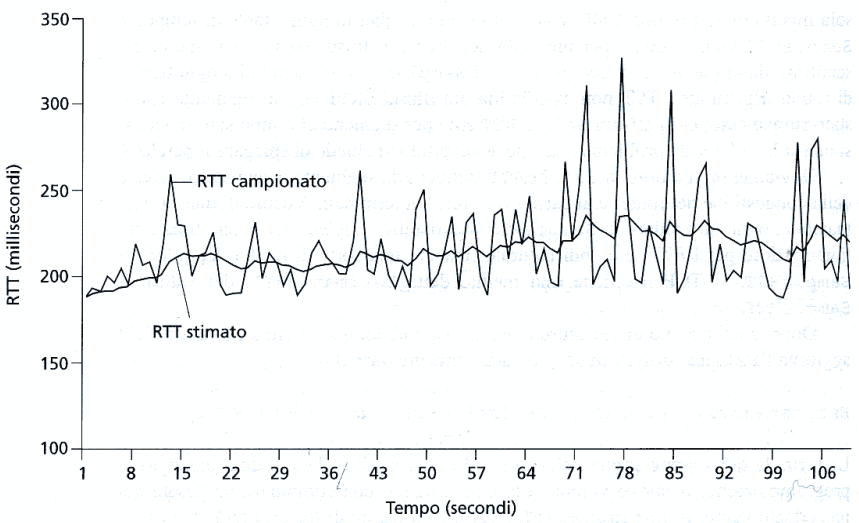
\includegraphics[scale=0.6]{img/032.png}
	\caption{RTT campionati e RTT stimati}
\end{figure}
Dati i valori \emph{EstimatedRTT} e \emph{DevRTT}, che valore dovrebbe essere usato per l'intervallo di timeout di TCP? Chiaramente l'intervallo dovrebbe essere maggiore o uguale a EstimatedRTT ma non troppo maggiore. È consigliabile impostare il timeout pari a EstimatedRTT pià un margine che dovrebbe essere grande quando ci sono fluttuazioni ampie nei valori di SampleRTT, piccolo in caso contrario. Il valore di DevRTT dovrebbe entrare in gioco qui. \emph{DevRTT} è la stima di quanto \emph{SampleRTT} generalmente si discosta da \emph{EstimatedRTT}
\begin{center}
	$DevRTT = (1 - \beta)*DevRTT_{precedente} + \beta*|SampleRTT - EstimatedRTT|$
	\textbf{$TimeoutInterval = EstimatedRTT + 4 * DevRTT$}
\end{center}
Dove $\beta$ è il numero di pacchetti considerati per la stima.
\subsubsection{Trasferimento affidabile dei dati}
Ricordiamo che il servizio IP è inaffidabile.\\
Il TCP crea un \textbf{servizio di trasferimento affidabile dei dati} sopra al servizio inaffidabile best effort fornito da IP. Vediamo che ci sono tre principali eventi legati alla trasmissione e ritrasmissione dei dati nel mittente TCP:
\begin{itemize}
	\item ricezione di dati dall'applicazione sovrastante
	\item timeout del timer: il timer viene avviato quando il segmento viene passato a IP e viene associato al più vecchio segmento non riscontrato. L'intervallo di scadenza per questo timer è il \emph{TimeoutInterval}
	\item ricezione di un ACK
\end{itemize}
\begin{figure}
	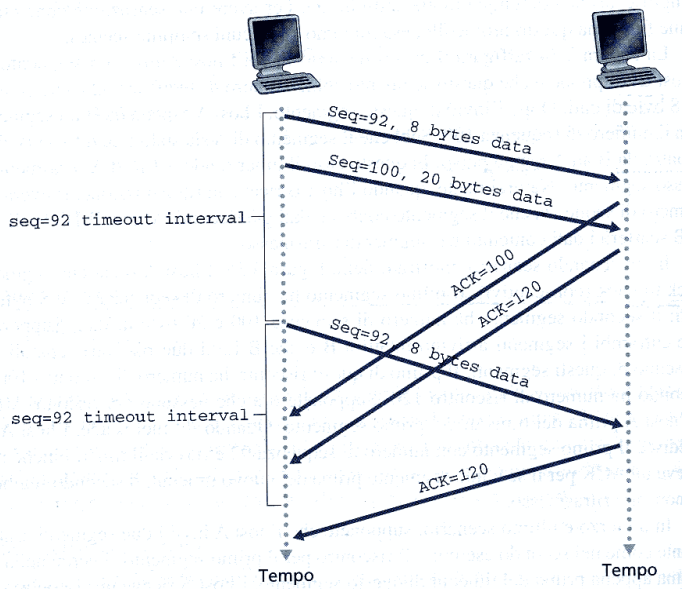
\includegraphics[scale=0.6]{img/033.png}
	\caption{Il segmento 100 non è ritrasmesso}
\end{figure}
\paragraph{Raddoppio dell'intervallo di timeout}
In questa modifica, quando si verifica un timeout, il TCP ritrasmette il segmento non ancora riscontrato con il più piccolo numero di sequenza ma, ogni volta che il TCP ritrasmette, esso imposta il prossimo intervallo di timeout al doppio del valore precedente. Quindi gli intervalli crescono esponenzialmente dopo ogni ritrasmissione. Comunque, ogni volta che il timer viene riavviato dopo uno dei due altri eventi, il \emph{TimeoutInterval} viene nuovamente derivato da \emph{EstimatedRTT} e \emph{DevRTT}. \\
Questa modifica fornisce una forma limitata di controllo della congestione.
\paragraph{Ritrasmissione veloce}
\begin{figure}
	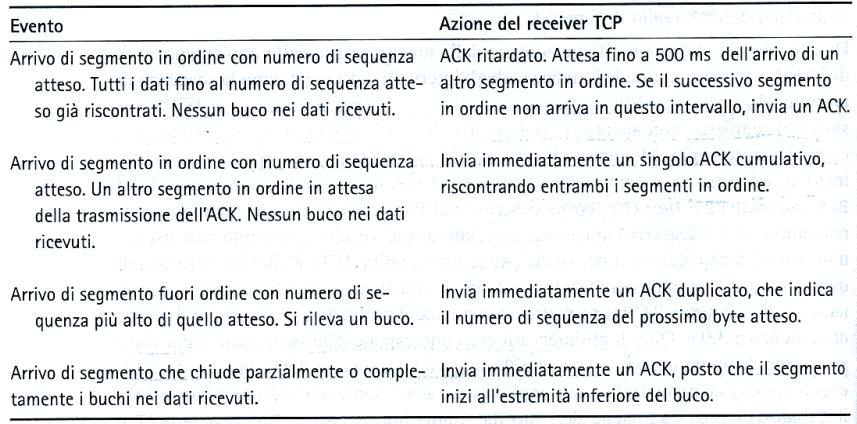
\includegraphics[scale=0.6]{img/034.png}
	\caption{Raccomandazioni per la generazione di ACK del TCP}
\end{figure}
Quando il mittente TCP riceve tre duplicati ACK per gli stessi dati, prende questa informazione come conferma che il segmento successivo a quello riscontrato tre volte è andato perso. In questo caso, TCP esegue una \textbf{ritrasmissione veloce}, ritrasmettendo il segmento mancante prima che il timer di quel segmento scada.
\paragraph{Go-Back-N o ripetizione selettiva?}
Ricordiamo che i riscontri TCP sono cumulativi e che i segmenti ricevuti correttamente ma guori sequenza non sono riscontrati individualmente dal ricevente. Quindi, TCP deve ricordare solo il più piccolo numero di sequenza di un byte trasmesso ma non riscontrato. In questo senso \textbf{TCP assomiglia molto a un protocollo in stile GBN}. Ci sono però delle differenze. Infatti, una modifica proposta per il TCP, il cosiddetto \textbf{riscontro selettivo}, consente a un ricevente TCP di riscontrare selettivamente segmenti fuori sequenza piuttosto che riscontrare cumulativamente l'ultimo segmento ricevuto correttamente, in sequenza. \\
Quindi, TCP è un ibrido tra i due sistemi.
\subsubsection{Controllo di flusso}
Ricordiamo che gli host riservano un buffer di ricezione per la connessione. Quando la connessione TCP riceve byte che sono costretti e in sequenza, colloca i dati nel buffer di ricezione. Il processo dell'applicazione associato leggerà i dati da questo buffer. Se l'applicazione è relativamente lenta nella lettura dei dati, il mittente potrebbe inviare troppi dati e potrebbe saturare il buffer di ricezione. \\
Il TCP fornisce alle sue applicazioni un \textbf{servizio di controllo del flusso}, ovvero un servizio di adattamento delle velocità. Questo controllo è detto \textbf{controllo della congestione}. \\
Il TCP fornisce il controllo di flusso attracerso il mantenimento nel mittente di una variabile detta \textbf{finestra di ricezione} \textit{(receive window)}. La finestra di ricezione è usata per dare al mittente un'idea di quanto spazio è disponibile nel buffer del ricevente. \textbf{La finestra di ricezione è dinamica}, ovvero varia durante la connessione. \\
Definiamo le seguenti variabili:
\begin{itemize}
	\item \emph{LastByteRead}: numer dell'ultimo byte nel flusso di dati letto dal buffer dal processo dell'applicazione in B
	\item \emph{LastByteRcvd}: numero dell'ultimo byte nel flusso di dati che è arrivato dalla rete ed è stato collocato nel buffer di ricezione in B
\end{itemize}
Poichè al TCP non è permesso di saturare il buffer assegnato, dobbiamo avere:
\begin{center}
	$LastByteRcvd - LastByteRead \leq RcvBuffer$
\end{center}
La finestra di ricezione, \emph{RcvWindow}, è posta uguale alla quantità di spazio disponibile nel buffer:
\begin{center}
	$RcvWindow = RcvBuffer - [LasstByteRcvs - LastByteRead]$
\end{center}
Poichè lo spazio disponibile cambia con il tempo, \emph{RcvWindow} è dinamica. \\
Come viene usata \emph{RcvWindow}? B inserisce in ogni segmento inviato ad A il valore attuale di \emph{RcvWindow}, inizialmente impostando $RcvWindow = RcvBuffer$. \\
L'host A a sua volta mantiene traccia di due variabili:
\begin{itemize}
	\item LastByteSent: ultimo byte inviato
	\item LastByteAcked: ultimo byte riscontrato
\end{itemize}
La differenza tra questi due è l'insieme dei byte non ancora riscontrati. \\
Poichè B invia dati ad A solo se deve inviare qualcosa o se deve dare riscontro, nel caso il buffer venisse svuotato ma B non dovesse inviare niente, allora A non saprebbe mai che il buffer si è svuotato. Per risolvere, A continua ad inviare segmenti con un byte di dati quando la finestra di ricezione di B è zero, in questo modo, quando saranno ricevuti dal buffer, B invierà un riscontro con la nuova \emph{RcvWindow}.
\subsubsection{Gestione della connessione TCP}
Ora vedremo come una connessione TCP viene instaurata e chiusa. \\
Supponiamo che un host A (client) voglia instaurare una connessione con un host B (server). Il processo del client informa il TCP che vuole stabilire una connessione con il server. Il TCP client procede allora a stabilirla nel seguente modo:
\begin{itemize}
	\item \textbf{Passo 1}: $TCP_{client}$ invia uno speciale segmento a $TCP_{server}$. Questo segmento non contiene dati dello strato di applicazione ma un bit del campo flag nell'intestazione, il cosiddetto SYN bit, è posto a 1. Inoltre il client sceglie un numero di sequenza iniziale (\emph{client\_isn}) e inserisce questo numero nel campo numero di sequenza del segmento iniziale SYN.
	\item \textbf{Passo 2}: Quando il datagram IP contenente il segmento SYN del $TCP_{client}$ arriva al server dell'host, il server estrae il segmento TCP dal datagram, determina il buffer TCP e le variabili alla connessione, e invia al client TCP un segmento che autorizza la connessione. Anche questo segmento non contiene dati dello strato di applicazione ma contiene tre informazioni:
		\begin{itemize}
			\item SYN posto a 1
			\item il campo di riscontro del segmento TCP è posto a client\_isn + 1
			\item il server sceglie il proprio numero iniziale di sequenza (\emph{server\_isn}) e colloca questo valore nel campo del numero di sequenza nell'intestazione TCP	
		\end{itemize}
		A volte ci si riferisce al segmento che autorizza la connessione come a un segmento \textbf{SYNACK}.
	\item \textbf{Passo 3}: Dopo la ricezione del segmento SYNACK, anche il client destina buffer e variabili alla connessione. L'host del client invia allora al server un ulteriore segmento. Quest'ultimo segmento riscontra il segmento che autorizza la connessione inserendo nel campo di riscontro \emph{server\_isn + 1}. Il bit SYN è posto a 0 perchè la connessione è stabilita
\end{itemize}
Questa è la procedura di \textbf{handshake a tre vie}.
\begin{figure}
	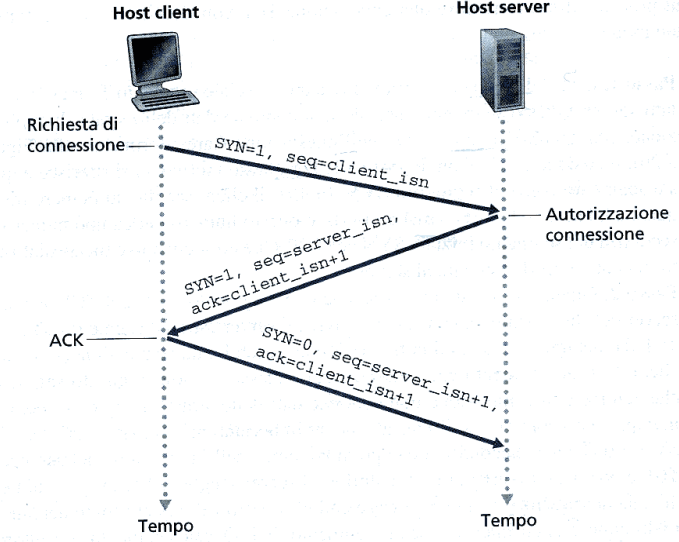
\includegraphics[scale=0.6]{img/035.png}
	\caption{Handshake a tre vie}
\end{figure}
\\
Ciascuno dei due processi che partecipano a una connessione TCP possono chiuderla. Quando viene chiusa, le risorse (buffer e variabili) negli host sono deallocate. \\
Il processo dell'applicazione imposta un comando di chiusura, questo fa sì che il TCP del client inviii nuo speciale segmento TCP al processo dell'altro host. Questo segmento speciale ha un bit nel campo flag dell'intestazione del segmento, il campo \textbf{FIN} posto a 1. Quando l'host riceve questo segmento, invia un ACK al mittente per poi a sua volta inviare un segmento di chiusura della connessione allo stesso modo. Il primo host a questo punto invia un ACK in risposta e tutti e due deallocheranno le risorse. \\
\begin{figure}
	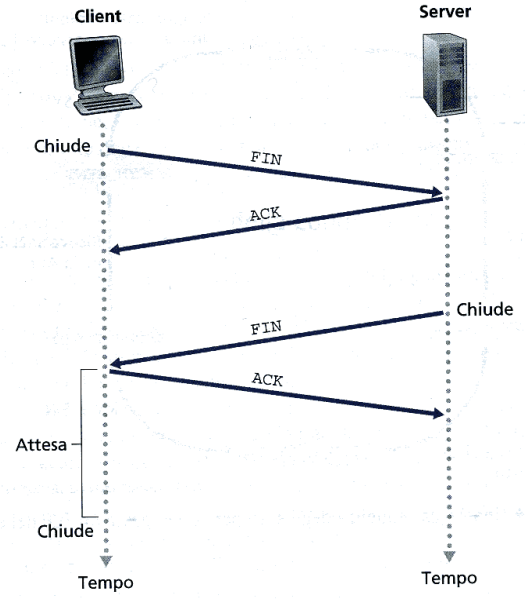
\includegraphics[scale=0.6]{img/036.png}
	\caption{Chiusura di una connessione TCP}
\end{figure}
Durante il periodo dell'esistenza della connessione tCP, il protocollo TCP funziona in ciascun host eseguendo transizioni tra vari \textbf{stati del TCP}. 
\begin{figure}
	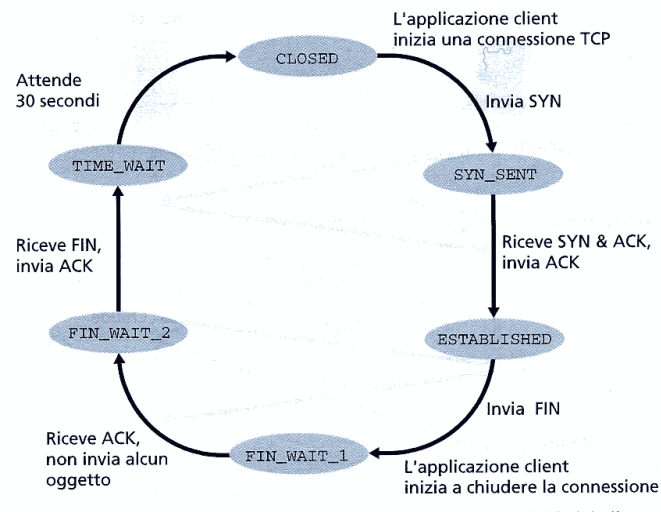
\includegraphics[scale=0.6]{img/037.png}
	\caption{Tipica sequenza degli stati per i quali passa un TCP del client}
	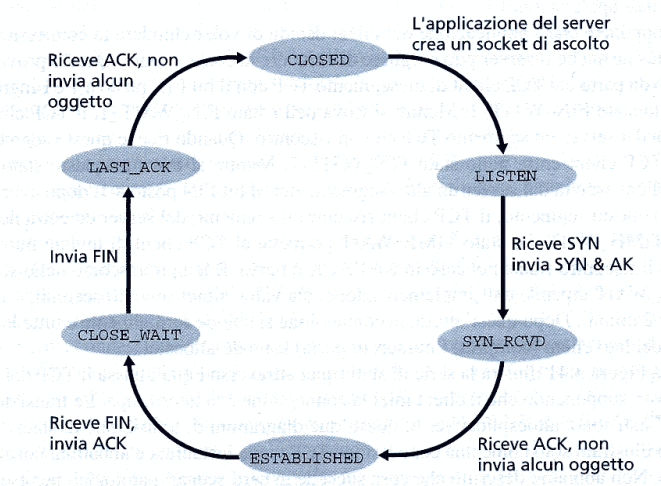
\includegraphics[scale=0.6]{img/038.png}
	\caption{Tipica sequenza degli stati per i quali passa un TCP del server, supponendo che sia il client a interrompere la connessione}
\end{figure}

\subsection{Principi del controllo della congestione}
Sappiamo che una delle cause principali della perdita di segmenti è la congestione della rete. La ritrasmissione dei segmenti cura l'effetto ma per correggere il problema alla radice servono sistemi che "strozzino" i sender nel caso di una congestione.
\subsubsection{Le cause e i costi della congestione}
Considereremo tre scenari di complessità crescente in cui si verifica la congestione. In tutti i casi valuteremo le cause della congestione e i suoi costi.
\paragraph{Scenario 1: due sender, un router con buffer infinito}
\begin{figure}
	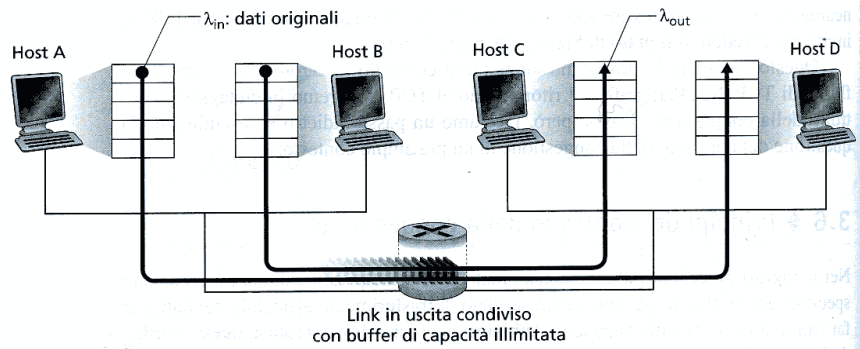
\includegraphics[scale=0.6]{img/039.png}
	\caption{Primo scenario di congestione: due connessioni dividono un singolo hop con buffer infinito}
\end{figure}
Due host (A e B), ciuscino con una connessione che condivide un singolo hop (salto, router) fra sorgente e destinazione.\\
Assumiamo che A stia inviando dati a una velocità media di $\lambda_{in}$ byte/s. Questi dati sono "originali", nel senso che ciascuna unità di dati è inviata nel socket una sola volta. I dati sono incapsulati e spediti. non viene eseguito alcun recupero degli errori (ad esempio ritrasmissione), controllo di flusso o controllo della congestione. Ignorando il carico addizionale dovuto all'aggiunt delle informazioni di intestazione, la velocità a cui l'host A offre il traffico al router in questo primo scenario è $\lambda_{in}$ byte/s. L'host B opera in maniera simile, quindi suppioniamo che stia inviando anch'esso dati alla velocità di $\lambda_{in}$ byte/s.\\
I pacchetti degli host A e B passano attraverso un router e su un link di uscita condiviso di capacità R. Il router ha buffer che permettono di incamerare i pacchetti in arrivo quando la velocità di arrivo supera la capacità di uscita. \\
\begin{figure}
	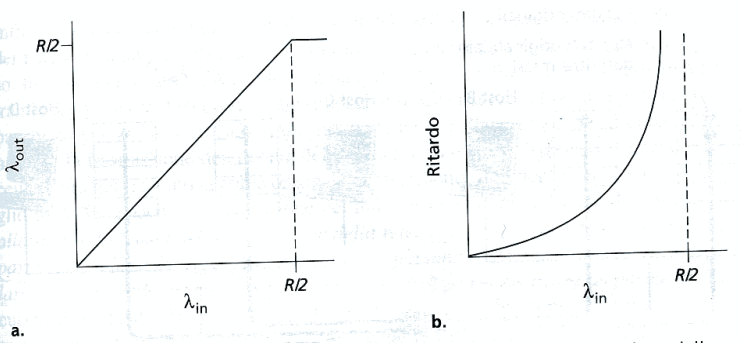
\includegraphics[scale=0.6]{img/040.png}
	\caption{Primo scenario di congestione:throughput e ritardo in funzione della velocità di spedizione dell'host}
\end{figure}
Il grafico riporta il \textbf{throughput per la connessione} (numero di byte al secondo al receiver) in funzione della velocità di spedizione dei dati: per una velocità fra 0 e R/2, il thorughput al receiver uguaglia la velocità di spedizione del sender. \\ \\
\textbf{Attenzione}: il limite superiore R/2 è una conseguenza della condivisione della capacità del link fra le due connessioni. Infatti, quando la velocità di spedizione supera R/2, il throughput è solo R/2. \\ \\
Quando la velocità di spedizione supera R/2, il numero medio di pacchetti in coda nel router diventa illimitato, e il rituardo emdio tra sorgente e destinazione diventa infinito (assumendo che la connessione vada avanti all'infinito). Quindi, operare vicino a R come velocità è certo ottimo per il throughput ma pessimo per il ritardo. \\
Abbiamo trovato il costo della congestione di rete in questo scenario: ci si devono aspettare grandi ritardi di coda quando la velocità di arrivo dei pacchetti è prossima alla capacità del link.
\paragraph{Scenario 2: due sender, un router con buffer finito}
\begin{figure}
	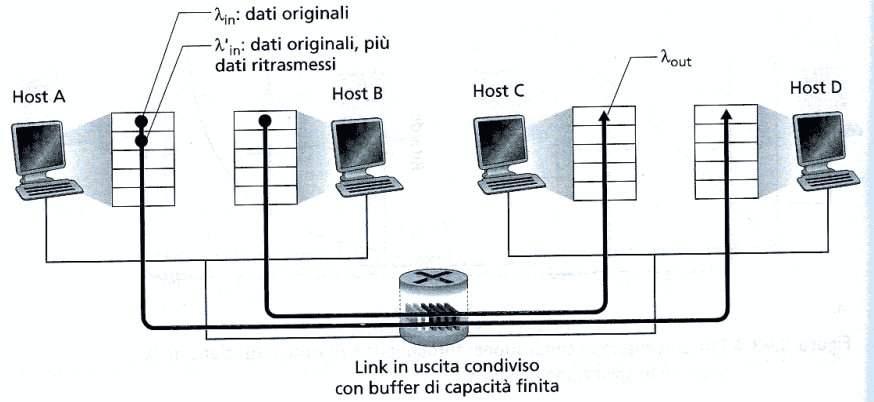
\includegraphics[scale=0.6]{img/041.png}
	\caption{Secondo scenario: due host (con ritrasmissioni) e un router con buffer finito}
\end{figure}
Assumiamo ora che il buffer del router sia finito. Una conseguenza di ciò è che i pacchetti in eccesso saranno scartati quando raggiungono un buffer pieno. Consideriamo anche che ciascuna connessione sia affidabile, ovvero che se un pacchetto viene perso dal router, sarà ritrasmesso dal mittente. Proprio per il fatto che i pacchetti possono essere rispediti dobbiamo stare attenti al termine "velocità di spedizione":
\begin{itemize}
	\item lo strato dell'applicazione invia dati a $\lambda_{in}$ byte/s
	\item lo strato di trasporto invia dati (originali e ritrasmessi) a $\lambda_{in}^{'}$ byte/s. Ci si riferisce a questa velocità come \textbf{carico offerto alla rete}
\end{itemize}
Ora, se il mittente potesse sapere se il buffer è pieno o no allora non ci sarebbero ritrasmissioni, portando a $\lambda_{in}^{'} = \lambda_{in}$. Questo caso è illustrato dalla retta superiore del grafico a sinistra. \\
Ora invece consideriamo il caso nel quale il sender rispedisca un pacchetto solo quando è sicuro che sia andato perso. In questo caso, le prestazioni potrebbero assomigliare a quelle del grafico a destra.
\paragraph{Scenario 2: due sender, un router con buffer finito}
\begin{figure}
	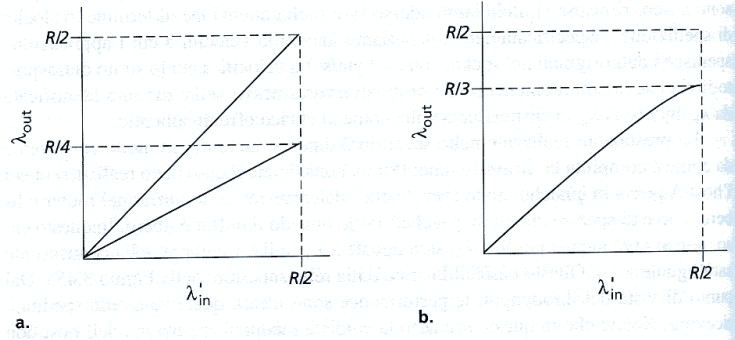
\includegraphics[scale=0.6]{img/042.png}
	\caption{Secondo scenario: prestazioni}
\end{figure}
Per capire, consideriamo il caso in cui il carico offerto $\lambda_{in}^{'}$ sia uguale a 0,5R. In accordo con la figura a destra, a questo valore di carico offerto la velocità dei dati spediti spediti all'applicazione del receiver è R/3. Allora, delle 0,5R unità di dati trasmessi, 0,333R byte/s (in media) sono dati originali e 0,166R byte/s (in media) sono dati ritrasmessi. \\
Vediamo qui un altro costo della congestione della rete: il sender deve eseguire ritrasmissioni per compensare i pacchetti scartati (dropped) a causa del sovraccarico del buffer. \\
Infine, consideriamo il caso nel quale il timer del sender scada prematuramente e il sender ritrasmetta il pacchetto che in realtà è stato ritardato dalla coda ma non è stato perso. In questo caso il lavoro fatto dal router nell'inoltrare la trasmissione della copia del pacchetto originale è sprecato. Il router, invece, avrebbe meglio usato la capacità di trasmissione del link per inviare un pacchetto diverso. \\
Ecco un altro costo della congestione di rete: le ritrasmissioni non necessarie a fronte di grandi ritardi portano il router a usare la larghezza di banda del suo link per inoltrare copie non necessarie. \\
La curva inferiore del grafico a sinistra mostra il throughput in funzione  del carico offerto quando si assume che ciascun pacchetto debba essere inoltrato (in media) due volte dal router, riducendo il valore asintotico a R/4.
\paragraph{Scenario 3: quattro sender, router con buffer finito e percorsi a salti multipli}
\begin{figure}
	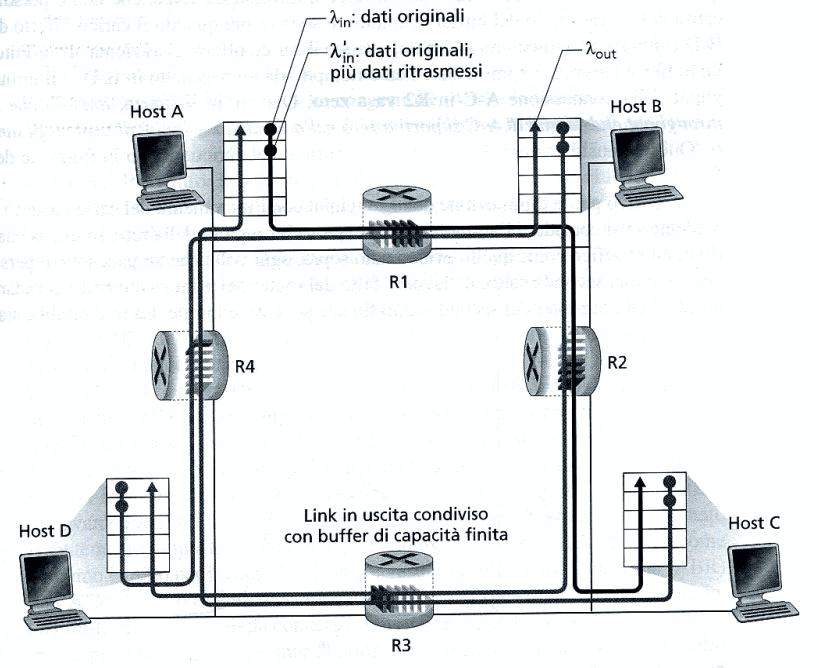
\includegraphics[scale=0.6]{img/043.png}
	\caption{Quattro sender, router con buffer finito e percorsi a salti multipli}
\end{figure}
Quattro host trasmettono pacchetti, ciascuno su percorsi di due salti sovrapposti. Assumiamo ancora che ciascun host usi un meccanismo di timeout/ritrasmissione per implementare un servizio di trasferimento affidabile dei dati, che tutti gli host abbiano lo stesso valore di $\lambda_{in}$ e che tutti i link dei router abbiano capacità R byte/s. \\
Consideriamo la connessione A-C, passando attraverso i router R1 e R2. La connessione A-C condivide R1 con D-B e R2 con B-D. per valori estremamente piccoli di $\lambda_{in}$, il sovraccarico del buffer è raro e il throughput è circa uguale al carico offerto. Per valori leggermente superiori di $\lambda_{in}$, il throughput corrispondente è anch'esso maggiore, e una maggior quantità di dati originali è trasmessa nella rete e raggiunge la destinazione, il sovraccarico è anche raro. Quindi, per piccoli valori di $\lambda_{in}$, un aumento di $\lambda_{in}$ si traduce in un aumento di $\lambda_{out}$. \\
Consideriamo ora il caso in cui $\lambda_{in}$ (e quindi $\lambda_{in}^{'}$ sia estremamente grande. Consideriamo il router R2. il traffico A-C in arrivo al router R2 può avere una velocità di arrivo che è al massimo R, la capcità del link da R1 a R2, indipendentemente dal valore di $\lambda_{in}$. Se $\lambda_{in}^{'}$ è estremamente grande per tutte le connessioni, allora la velocità di arrivo del traffico di B-D a R2 può essere più grande di quella del traffico A-C. Poichè il traffico di A-C e quello di B-D devono competere al router R2 a causa del limitato spazio di buffer, la quantità del traffico di A-C che con successo attraversa R2 diminuscie sempre più quando il carico offerto da B-D continua ad aumentare. Al limite, quando il carico offerto si avvicina all'infinito, un buffer vuoto in R2 è immediatamente riempito da un pacchetto di B-D, e il throughput della connessione A-C in R2 va a zero. \\
Questo, in sostanza, implica che il throughput end-to-end di A-C si porti a zero nella condizione limite di traffico pesante. \\
\begin{figure}
	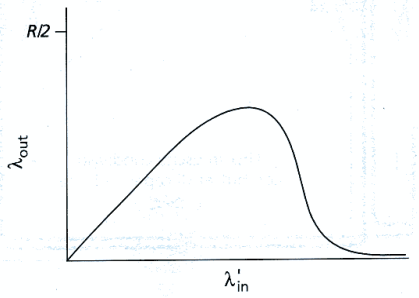
\includegraphics[scale=0.6]{img/044.png}
	\caption{Terzo scenario: prestazioni con buffer finito e percorsi a salti multipli}
\end{figure}
Il motivo per la diminuzione del throughput con l'incremento del carico offerto è evidente se sis considera l'ammontare del lavoro compiuto dalla rete. Se R2 si trova a scartare un pacchetto, allora il lavoro di R1 è stato sprecato. \\
Qui possiamo vedere ancora un altro costo della perdita di un pacchetto dovuta alla congestione: quando un pacchetto è perso lungo un percorso, la capacità di trasmissione che è stata usata in ciascuno dei router a monte per inoltrare quel pacchetto al punto in cui si è perso è stata sprecata.

\subsection{Controllo della congestione del TCP}
Le due componenti più importanti di TCP sono:
\begin{itemize}
	\item fornisce un servizio di trasporto affidabile
	\item ha un meccanismo di controllo della congestione
\end{itemize}
L'approccio seguito da TCP è di fare sì che ogni mittente limiti il ritmo a cui immette traffico nella sua connessione in funzione della congestione in rete percepita. Se un mittente TCP percepisce che c'è poca congestione nel percorso tra sè e la destinazione, allora il mittente TCP aumenta il suo ritmo di trasmssione; se il mittente percepisce che c'è congestione lungo il percorso, allora il mittente riduce il suo ritmo di invio. Ma questo approccio solleva tre problemi:
\begin{itemize}
	\item in che modo il mittente TCP limita il ritmo a cui manda traffico nelle sue connessioni?
	\item come un mittente TCP percepisce che c'è congestione nel percorso tra sè e la destinazione?
	\item quale algoritmo dovrebbe utilizzare il mittente per cambiare il suo ritmo di invio in funzione della congestione end-to-end percepita?
\end{itemize}
Esamineremo prima in che modo un mittente limita il ritmo al quale invia traffico nella sua connessione. Il meccanismo di controllo della congestione del TCP da entrambi i lati della connessione deve tener traccia di un'altra variabile: la \textbf{finestra di congestione} \textit{(congestion window)}. La finestra di congestione impone una limitazione addizionale alla quantità di traffico che un host può inviare in una connessione. Specificatamente, l'ammontare dei dati non riscontrati che un host può avere all'interno di una connessione TCP non deve superare il minimo tra CongWin e RcvWin, che è:
\begin{center}
	$LastByteSent - LastByteAcked \leq min{CongWin, RcvWindow}$
\end{center}
Per porre l'attenzione sul controllo della congestione assumiamo che il buffer di ricezione del TCP sia abbastanza grande da poter ignorare il vincolo della finestra di ricezione. In questo caso, la quantità di dati non riscontrati che un host può avere all'interno di una connessione TCP è limitata unicamente attraverso \emph{CongWin}. \\
Consideriamo una connessione per cui l perdita e i ritardi di trasmissione dei pacchetti siano trascurabili. Quindi, approssimativamente, all'inizio di ogni tempo di round-trip\footnote{Il Round Trip Time (acronimo RTT) nelle telecomunicazioni è il tempo che intercorre tra l'invio di un segnale più il tempo necessario per la ricezione della conferma di quel segnale.} (RTT), il limite sopra esposto permette al mittente di inviare \emph{CongWin} byte di dati nella connessione, e alla fine del RTT il mittente riceve i riscontri per i dati. \\
Quindi il ritmo di invio del mittente è circa \emph{CongWin/RTT} byte/s. \\
Definiamo un \textit{"evento di perdita"} a un mittente TCP come il verificarsi o di un timeout o della ricezione di tre ACK duplicati dal ricevente\footnote{Che, come abbiamo detto precedentemente, porta alla ritrasmissione veloce dei pacchetti ancora senza ACK}. Quando c'è troppa congestione vi è perdita di datagrammi. Il datagram perso, a sua volta, dà luogo a un evento di perdita al mittente, o a un timeout o la ricezione di tre ACK duplicati, che è considerato dal mittente come un'indicazione della congestione del percorso. \\
Ora siamo in grado di considerare l'algoritmo che un mittente TCP usa per regolare il suo ritmo di invio in funzione della congestione percepita, ovvero l'\textbf{algoritmo di controllo della congestione di TCP}. L'algoritmo ha tre componenti principali:
\begin{itemize}
	\item incremento adattivo, decremento moltiplicativo
	\item partenza lenta (\textit{slow start})
	\item reazione a eventi di timeout
\end{itemize}
\paragraph{Incremento adattivo, decremento moltiplicativo}
L'idea alla base del controllo di congestione di TCP è quella di far ridurre al mittente il suo ritmo di invio (diminuendo la dimensione della sua finestra di congestione, \emph{CongWin}) quando si verifica un evento di perdita. Ma di quanto il mittente TCP deve ridurre la sua finestra di congestione quando si verifica un evento di perdita? Il TCP usa un approccio detto \textbf{"decremento moltiplicativo"}, che dimezza il valore attuale di \emph{CongWin} dopo un evento di perdita. Quindi, se il valore di \emph{CongWin} è attualmente di 20 kbyte e si verifica una perdita, \emph{CongWin} viene dimezzato a 10 kbyte. Il valore di \emph{CongWin} può continuare a scendere, ma non può scendere sotto a un MSS. Questa è una spiegazione MOLTO semplificata come vedremo dopo. \\
Consideriamo ora come TCP debba aumentare il ritmo di invio se non percepisce congestione, ovvero quando non ci sono perdite. In questo caso TCP aumenta lentamente la sua finestra di congestione. Il mittente fa questo ogni volta che riceve un ACK, approssimativamente aumentandola di un MSS per ogni RTT fin quando non si verificano eventi di perdita. \\
Quindi TCP aumenta additivamente \textbf{($CongWin = CongWin_{prec} + MSS$)} e riduce moltiplicativamente \textbf{($CongWin = CongWin_{prec}/2$)}. Per questo motivo, il controllo di congestione di TCP è spesso definito come un \textbf{algoritmo a incremento adattivo, decremento moltiplicativo (AIMD)}. La fase di incremento lineare del protocollo di controllo della congestione è nota come \textbf{prevenzione della congestione} \textit{(congestion avoidance)}
\begin{figure}
	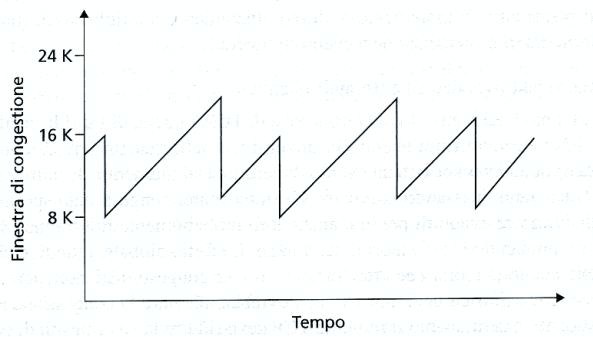
\includegraphics[scale=0.6]{img/045.png}
	\caption{Algoritmo di controllo della congestione a incremento additivo-decremento moltiplicativo}
\end{figure}
\paragraph{Partenza lenta (slow start)}
Quando si inizia una connessione TCP il valore di CongWin è inizializzato a un MSS, dando luogo a un ritmo iniziale di invio pari approssimativamente a \emph{MSS/RTT}. Per esempio, se MSS = 500 byte e RTT = 200 ms, allora il ritmo iniziale è solo circa 20 kbit/s. Dato che la banda potrebbe essere molto maggiore di MSS/RTT, sarebbe uno spreco aumentare il ritmo linearmente. Quindi, invece di incrementare il suo ritmo linearmente durante questa fasse iniziale, un mittente TCP \textbf{aumenta il suo ritmo a velocità esponenziale, raddoppiando il valore di \emph{CongWin} ogni RTT}. Al primo segnale di congestione si entra nel regime normale AIMD. Quindi, durante questa fase iniziale, chiamata \textbf{partenza lenta}, il mittente TCP inizia trasmettendo a un ritmo lento ma aumentando a velocità esponenziale.
\paragraph{Reazioni a eventi di timeout}
Il quadro presentato fino ad ora è incompleto, poichè TCP si comporta in maniera differente se la congestione è rilevata attraverso un evento di timeout e non attraverso tre ACK consecutivi. \textbf{Dopo un evento di timeout, il mittente TCP entra in una fase di partenza lenta}. \\
Il TCP gestisce queste dinamiche più complesse mettendo una variabile chiamata \textbf{\emph{Threshold}} \textit{(soglia)}, che determina la dimensione della finestra alla quale deve terminare la partenza lenta, e deve cominciare la prevenzione della congestione. La variabile \emph{Threshold} è inizialmente posta a un valore grande (65 kbyte) in modo che non abbia alcun effetto iniziale. Quando si verifica un evento di perdita, \emph{Threshold} è posto pari alla metà del valore attuale di \emph{CongWin}. Per esempio, se \emph{CongWin} è 20 kbyte, allora \emph{Threshold} viene posto a 10 kbyte e conserverà questo valore fino al successivo evento di perdita. \\
Ora descriviamo come si comporta \emph{CongWin} dopo un evento di timeout:
\begin{itemize}
	\item \textbf{Fase iniziale}: partenza lenta, $CongWin = CongWin_{prec}*2$
	\item \textbf{Raggiungimento \emph{CongWin = Threshold}}: AIMD, $CongWin = CongWin_{prec} + MSS$
	\item \textbf{Evento di perdita, tipo ACK duplicato tre volte}: $CongWin = CongWin_{prec}/2$, $Threshold = CongWin_{prec}/2$
	\item \textbf{Evento di timeout}: $CongWin = MSS$, $Threshold = CongWin_{prec}/2$, ricomincia la partenza lenta
\end{itemize}
Questo meccanismo è proprio della nuova versione di TCP, \textbf{TCP Reno}. Nella versione precedente, \textbf{TCP Tahoe}, per ogni evento di perdita si impostava \emph{CongWin = MSS}.
\begin{figure}
	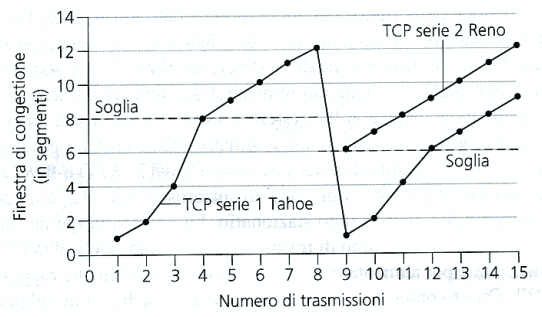
\includegraphics[scale=0.6]{img/046.png}
	\caption{Evoluzione della finestra di congestione del TCP}
\end{figure}
\paragraph{Descrizione macroscopica del throughput di TCP}
Dato l'andamento di TCP, è naturale considerare quale possa essere il throughput medio di una connessione di lunga durata. Per questa analisi ignoriamo le fasi di partenza lenta e le perdite.\\
Quando la dimensione della finestra è di w byte e il tempo di round-trip è uguale a RTT secondi, il ritmo di trasmissione di TCP è circa w/RTT. Fino ad un evento di perdita, w viene aumentato di un MSS per ogni RTT. Indichiamo con W il valore di w quando si verifica una perdita. Assumendo che W e RTT siano approssimativamente costanti, il ritmo di trasmissione di TCP varia tra \emph{$W/(2 * RTT)$ e $W/RTT$}. Poichè il throughput aumenta linearmente fra due valori estremi, abbiamo:
\begin{center}
	Throughput medio di una connessione = $\dfrac{0,75 * W}{RTT}$
\end{center}
\subsubsection{Fairness}
Consideriamo K connessioni TCP, ciascuna con un diverso percorso da estremo a estremo, ma tutte passanti attraverso un link collo di bottiglia\footnote{Ovvero è l'unico congestionato e gli altri hanno capacità trasmissiva in abbondanza rispetto a questo} \textit{(bottleneck)} con ritmo di trasmissione pari a R bit/s. Supponiamo che ogni connessione stia trasferendo un grande file e non ci sia traffico UDP che passa attraverso il link collo di bottiglia. Un meccanismo di controllo della congestione è detto \textbf{fairness}, ovvero essere fair (equo) se il ritmo di trasmissione medio di ogni connessione è approssimativamente pari a R/K, cioè, ogni connessione ottiene un'uguale porzione della banda del link. \\
\textbf{AIMD è fair? Sì.} Consideriamo due conenssioni TCP che condividono un singolo link con velocità di trasmissione R.
\begin{figure}
	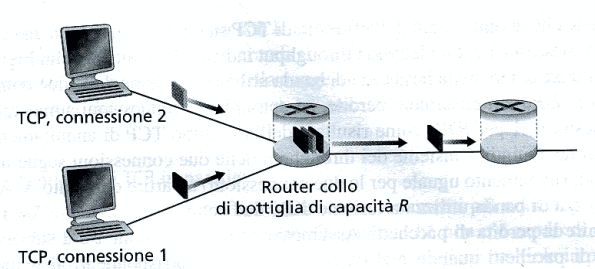
\includegraphics[scale=0.6]{img/047.png}
	\caption{Due connessioni TCP condividono la banda di un singolo link collo di bottiglia}
\end{figure}
Supponiamo che le due connessioni abbiano gli stessi MSS e RTT, che entrambe abbiano una grande quantità di dati da spedire e che nessun'altra connessione TCP o datagram UDP attraversino il link condiviso. Ignoriamo anche la partenza lenta e assumiamo che le connessioni TCP operino in modalità AIMD tutto il tempo.
\begin{figure}
	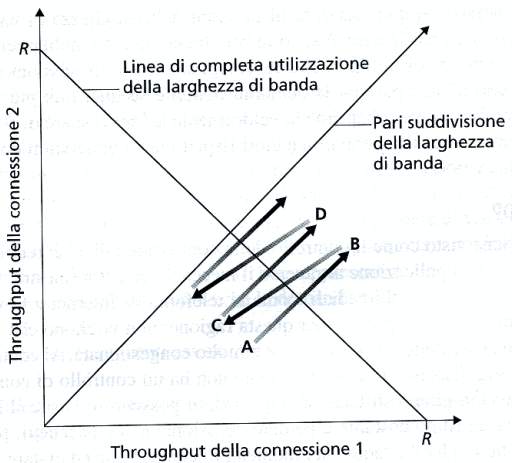
\includegraphics[scale=0.6]{img/048.png}
	\caption{Throughput realizzati dalle connessioni TCP 1 e 2}
\end{figure}
Se le due connessioni TCP condividono equamente la larghezza di banda del link, allora il throughput ottenuto cadrà sulla freccia a 45 gradi (pari suddivisione della larghezza di banda). \\
Supponiamo che le dimensioni della finestra di TCP siano quelle per cui a un certo tempo, le connessioni 1 e 2 realizzino i throughput indicati dal punto A. Poichè l'ammontare della larghezza di banda utilizzata insieme dalle due connessioni è inferiore a R, non ci saranno perdite, ed entrambe continueranno ad aumentare \emph{CongWin} di un MSS per ogni RTT, procedendo su di una linea crescente a 45 gradi. Alla fine la somma dei due throughput sarà superiore a R come evidenziato nel punto B, allora entrambe le connessioni ridurranno a metà la loro \emph{CongWin}, portandosi a C e così via, mantenendo un equilibrio. \\
Questo è un caso molto irrealistico, infatti, ad esempio, la connessione con RTT inferiore aumenterà più velocemente, ottenendo la maggior parte della rete.
\paragraph{Fairness e UDP}
Molte applicazioni multimediali, come la telefonia su internet e le video conferenze, non girano su TCP proprio per questa ragione: non vogliono che il loro ritmo di trasmissione sia ridotto, anche se la rete è molto congestionata. Per questo girano su UDP, in questo modo possono aumentare costantemente la loro velocità senza problemi, sopportando alcune perdite di pacchetti. Dal punto di vista di TCP, le connessioni UDP non sono eque.
\paragraph{Fairness e connessioni TCP in parallelo}
TCP può non essere fair se l'applicazione sfrutta più connessioni TCP in parallelo. Per esempio i browser usano più connessioni per caricare le pagine. Per fare un esempio, immaginiamo che ci siano 9 connessioni TCP singole, tutte avranno R/9 di velocità di trasmissione. Se si aggiungesse una nuova applicazione diventerebbero 10, portando la velocità a R/10 per tutti. Se questa nuova applicazione, però, usasse 11 connessioni parallele, riuscirebbe a prendersi R/2 della banda possibile.

\section{Livello di rete: piano dei dati}
\subsection{Introduzione}
\begin{figure}
	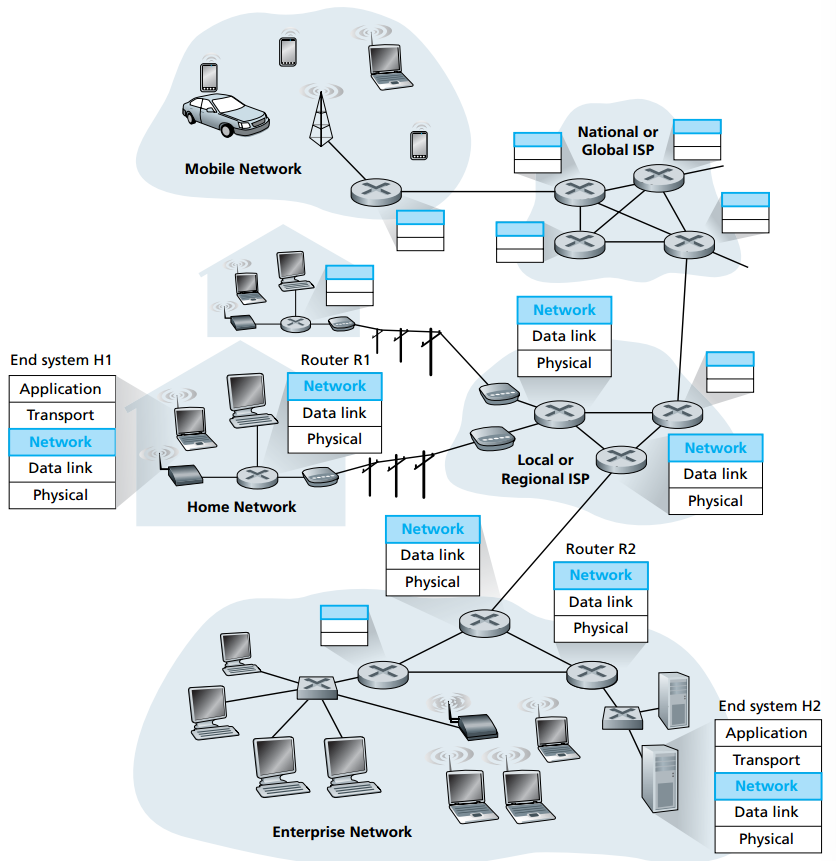
\includegraphics[scale=0.6]{img/049.png}
	\caption{Lo strato di rete}
\end{figure}
Nell'immagine abbiamo due host, H1 e H2, e svariati router sul loro percorso. Supponiamo che H1 sia il mittente e H2 il destinatario e consideriamo il ruolo dello strato di rete. \\
lO strato di rete di H1 prende il segmento dallo strato di trasporto, incapsula ogni segmento in un datagram (che è il tipo di pacchetto dello strato di rete, e lo invia al primo router, R1. H2, quando riceve il datagram, estrae il segmento e lo invia allo strato di trasporto. Il ruolo primario dei router e di spedire (forward) i datagrammi da link di input a quello di output.
\subsubsection{Forwarding e Routing}
Il ruolo dello strato di rete è semplice: spostare i pacchetti tra i vari host. Per fare ciò si identificano due funzioni importanti:
\begin{itemize}
	\item \textbf{Forwarding}: quando un pacchetto arriva al link di input, il router semplicemente sposta il link all'appropriato link di output
	\item \textbf{Routing}: Lo strato di network deve determinare il percorso che i pacchetti devono prendere affinchè arrivino dal mittente al ricevente. L'algoritmo che calcola questi percorsi si chiama \textbf{"algoritmo di routing"}.
\end{itemize}
Il termine forwarding si riferisce all'azione locale di trasferire i pacchetti mentre routing si riferisce al processo che coinvolge tutto il network. \\
Ogni router ha una \textbf{tabella di forwarding}. Un router inoltra il pacchetto esaminando il valore do un campo dell'header del pacchetto e poi usando questo valore per indicizzarlo nella tabella di forwarding. Il valore immagazzinato nella tabella di forwarding indica l'interfaccia del link di output sul quale deve essere instradato il pacchetto.
Nella figura viene mostrato il funzionamento della tabella di forwarding: il pacchetto arriva con un'intestazione, questa viene cercata all'interno della tabella e determina il link da prendere.
\begin{figure}
	\begin{center}
		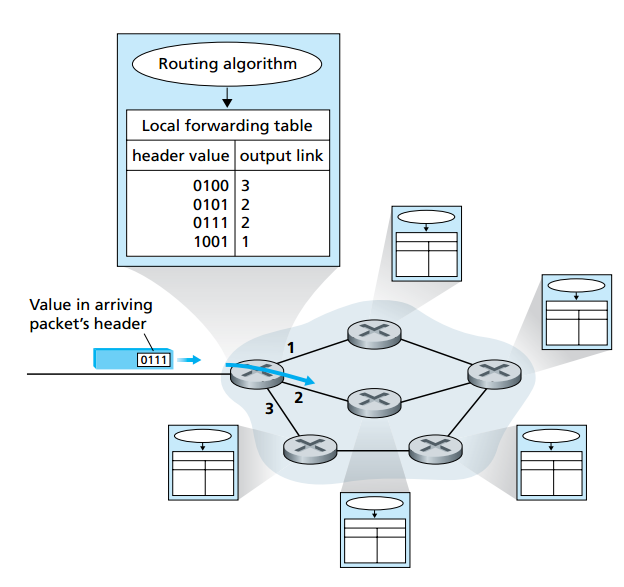
\includegraphics[scale=0.6]{img/050.png}
		\caption{L'algoritmo di routing determina il valore nella tabella di forwarding}
	\end{center}
\end{figure}
Come vengono determinati i valori della tabella di routing? L'algoritmo determina i valori che sono inseriti nella tabella. L'algoritmo può essere centralizzato (risiede su di un router che poi invia le informazioni ai router periferici) o decentralizzato (in ogni router). \\
Per impostare la terminologia, da qui useremo \textbf{packet switch} per indicare un dispositivo generico di packet-witching che trasferisce i pacchetti da un link all'altro. Alcuni packet switch, chiamati \textbf{link-layer switches}, basano le loro decisioni di forwarding sul valore nel campo del frame dello strato di collegamento, altri packet-switch, i \textbf{router} basano la loro decisione sul valore del campo dello strato di rete.
\paragraph{Impostazione della connessione}
In alcuni network di computer lo strato di network ha una terza funzione: \textbf{l'impostazione della connessione} (\textit{Connection setup}). La funzione è simile a quella dell'handshake, semplicemente viene eseguita tra tutti i router del percorso in modo che i pacchetti possano scorrere tra di essi.
\subsubsection{Modelli di servizio di network}
Quando il livello di trasporto trasmette un pacchetto al livello di rete, può fare affidamento sul livello di rete per inviare il pacchetto alla sua destinazione? Quando più pacchetti sono spediti, arriveranno tutti in ordine? L'intervallo di tempo tra l'invio sequenziale di due pacchetti sarà uguale all'intervallo di ricezione? La rete offrirà un feedback sulla congestione? \\
La risposta a queste domande e altre sono determinate dal modello di servizio offerto dal livello di rete. Il \textbf{modello di servizio di rete} definisce le caratteristiche del trasporto end-to-end. \\
Consideriamo ora alcuni servizi che il livello di rete può offrire. Il livello di trasporto del mittente, quando passa il segmento al livello di rete, specifica quali servizi includere:
\begin{itemize}
	\item \textbf{Spedizione garantita}: il servizio garantisce che il pacchetto arriverà
	\item \textbf{Spedizione garantita con un ritardo massimo}: il servizio non solo garantisce la spedizione del pacchetto, ma consegnata entro entro un specifico limite di ritardo host-to-host
\end{itemize}
Per di più, i seguenti sevizi possono essere offerti ad un flusso dati:
\begin{itemize}
	\item \textbf{Arrivo in ordine}: il servizio garantisce che i pacchetti arriveranno nell'ordine di invio
	\item \textbf{Banda minima garantita}: emula il comportamento del link di trasmissione, garantendo che sotto quella velocità di invio non ci sarà perdita di pacchetti e ogni pacchetto arriverà entro un certo ritardo (ad esempio, 40 millisecondi)
	\item \textbf{Massimo jitter garantito}: il servizio garantisce che l'ammontare di tempo tra due pacchetti successivi è uguale all'ammontare di tempo tra i loro arrivi a destinazione
	\item \textbf{Servizio di sicurezza}: usando una chiave segreta per la sessione che solo i due host conoscono, il livello di rete del mittente può criptare i pacchetti che poi saranno decriptati dal ricevente.
\end{itemize}
Il livello di rete di internet offre un solo servizio, conosciuto come \textbf{best-effort} (al meglio delle possibilità). Un servizio Best-effort è uguale a dire che è un servizio senza garanzie, infatti anche se non arrivassero mai i pacchetti allora il servizio sarebbe comunque best-effort.
\begin{figure}
	\includegraphics[scale=0.6]{img/051.png}
	\caption{I modelli di servizio di internet, ATM CBR e ATM ABR. ATM = Asynchronous Transfer Mode, CBR = constant bit rate, ABR = Available bit rate}
\end{figure}

\subsection{Il protocollo di internet (IP): forwarding e indirizzamento (addressing) in internet}
Ci sono due versioni di IP oggi, IPv4 e IPv6. Noi studieremo solo IPv4.
\subsubsection{Formato dei datagrammi IPv4}
\begin{figure}
	\begin{center}
		\includegraphics[scale=0.6]{img/052.png}
		\caption{Datagram IPv4}
	\end{center}
\end{figure}
Ricordiamo che un pacchetto del livello di rete è detto "datagram". \\
I campi chiave di un datagram IPv4 sono:
\begin{itemize}
	\item Numero di versione: questi 4 bit specificano la versione dl protocollo IP per sapere come identificare i seguenti campi
	\item \textbf{lunghezza dell'header}: questi 4 bit determinano da che punto il datagram inizia veramente
	\item \textbf{Tipo di servizio (TOS)}: servono a distinguere i vari tipi di datagram
	\item\textbf{ Lunghezza del datagram}: mostra la lunghezza del datagram, dati e header compresi
	\item Identificatori, flag, offset di frammentazione
	\item \textbf{Time-to-live (TTL}): imposta un massimo di vita al datagram, in modo che non rimanga in rete per sempre. Questo valore viene decrementato di 1 ogni volta che il datagram è processato da un router. Se il TTL arriva a 0, il datagram viene scartato
	\item \textbf{Protocollo}: questo campo viene usato solo quando il datagram arriva a destinazione. il valore di questo campo indica il protocollo specifico del livello di trasporto da usare (TCP o UDP)
	\item \textbf{Checksum}: come per i segmenti di UDP e TCP
	\item \textbf{Indirizzi IP di arrivo e destinazione}
	\item \textbf{Opzionali}: permettono l'estensione dell'header
	\item \textbf{Dati} (payload)
\end{itemize}
\subsubsection{Frammentazione dei datagrammi IPv4} \label{par: MTU}
Il massimo ammontare di dati che un frame del livello di collegamento può trasportare è chiamato \textbf{"unita massima di trasmissione"} \textit{(MTU)}. Poichè ogni datagram IP è incapsulato in un frame del livello di collegamento per il trasporto da un router all'altro, allora l'MTU del protocollo del livello di collegamento pone un limite alla lunghezza del datagram IP. Il vero problema, però, non è questo limite ma il fatto che i vari router sul percorso possano utilizzare differenti protocolli con differenti MTU. Supponiamo che ci arrivi un pacchetto di data dimensione e che questo debba essere indirizzato verso un altro link ma, problema, questo ha un MTU inferiore rispetto a quello in entrata. Che fare? La soluzione è la frammentazione dei dati nel datagram IP in due più piccoli datagram IP, ognuno incapsulato in un datagram più piccolo in un frame separato. Ognuno di questi datagram è chiamato \textbf{frammento}. \\
Per non aggiungere lavoro ai router, IPv4 non fa riassemblare i frame a questi ma è computo dell'host destinatario. Per riassemblarli, però, il sistema necessita di sapere se:
\begin{itemize}
	\item i frame fanno parte di un frame più grande
	\item se ha ricevuto tutti i frame
	\item come questi debbano essere riassemblati
\end{itemize} 
Per risolvere questo problema, IPv4 setta i campi di identificazione, flag e offset di frammentazione nell'intestazione. Quando un datagram viene creato, il mittente mette un numero di identificazione, l'IP di arrivo e di destinazione all'interno dell'intestazione. Tipicamente, ogni volta che viene creato un datagram il numero di identificazione viene incrementato di 1. Quando il datagram viene frammentato, vengono inseriti tutti questi campi e il numero di identificazione è uguale per tutti i frammenti, in questo modo il ricevente sa quando più frame fanno parte dello stesso frame originale. \\
Poichè IP non è affidabile, quindi affinchè il ricevente sappia di aver effettivamente ricevuto l'ultimo frammento, il flag di questo è impostato a 0, mentre tutti gli altri hanno flag uguale a 1. In più l'offset permette di capire se il frammento è all'interno del datagram IP originale. \\
Per fare un esempio, immaginiamo che un datagram di 4000 byte (20 byte di intestazione più 3980 byte di dati) arrivi ad un router e debba essere inoltrato su di un link con MTU di 1500 byte. Dobbiamo quindi frammentare il datagram in 3 frammenti. Supponiamo che il numero di identificazione sia 777. Le caratteristiche dei tre frammenti sono descritti dall'immagine.
\begin{figure}
	\begin{center}
		\includegraphics[scale=0.5]{img/053.png}
		\caption{Frammenti IP}
	\end{center}
\end{figure}
Alla destinazione, i dati vengono passati al livello di trasporto solo dopo che lo strato di collegamento ha ricostruito i datagram IP. Se non arrivano completi vengono scartati. Nel caso venga usato TCP, allora ci penserà questo a occuparsi della ritrasmissione dei paccehtit mancanti.
\subsubsection{Indirizzamento IPv4}
Generalmente un host ha un solo colelgamento con la rete; quando l'implementazione di IP dell'host vuole inviare un datagramma, lo fa su tale collegamento. Il confine tra host e collegamento fisico viene detto interfaccia. \\
Differentemente, poichè un router deve poter ricevere ed inviare datagrammi, deve avere almeno due collegamenti. Infatti il router presenta un'interfaccia per ogni collegamento. \\
IP richiede che ogni interfaccia abbia un proprio indirizzo, pertanto l'indirizzo IP è associato all'interfaccia e non all'host. Gli indirizzi IP sono lunghi 32 bit (4 byte) e quindi si possono avere $2^{32}$ indirizzi, circa 4 miliardi. Tali indirizzi sono solitamente scritti in notazione decimale puntata, ovvero dove i byte sono separati da un singolo punto. \\
Ogni interfaccia di host e router di internet ha un indirizzo IP globalmente univoco (eccetto se gestite da NAT, cosa che vedremo poi). Una parte dell'indirizzo di un'interfaccia è determinata dalla sottorete cui è collegata.
\begin{figure}
	\includegraphics[scale=0.5]{img/054.png}
	\caption{Indirizzi delle interfacce e sottoreti}
\end{figure}
La figura mostra un router con tre interfacce (223.1.1.4, 223.1.2.9, 223.1.3.27) che connette sette host. I tre a sinistra e l'interfaccia del router cui sono connessi hanno un indirizzo IP nella forma 233.1.1.xxx, ossia i 24 bit a sinistra sono identici a quelli della loro interfaccia. Per IP, questa rete che interconnette tre interfacce di host e l'interfaccia di un router forma una \textbf{sottorete}. IP ha quindi assegnato a questa sottorete l'indirizzo 223.1.1.0/24, dove la notazione /24 è detta \textbf{maschera di sottorete (subnet mask)} e indica che i 24 bit più a sinistra dell'indrizzo definiscono l'indirizzo della sottorete. Di conseguenza la sottorente è composta da tre interfacce di host e una di router (numerata per ultima). \\
\begin{figure}
	\includegraphics[scale=0.6]{img/055.png}
	\caption{Tre router che interconnettono sei sottoreti}
\end{figure}
Prendiamo il secondo caso dove abbiamo 3 router connessi da collegamenti punto a punto. Ciascuno ha tre interfacce (due per collegarsi agli altri router e una per la sottorete). Abbiamo quindi altre sottoreti che collegano i router tra di loro (ad esempio tra R1 ed R2 c'è la sottorete 223.1.9.xxx/24).
\begin{center}
	\textit{Per determinare le sottoreti si sgancino le interfacce da host e router in maniera tale da creare isole di reti isolate delimitate dalle interfacce. Ognuna di queste reti isolate viene detta sottorete (subnet)}
\end{center}
Cerchiamo di comprendere il meccanismo generale di assegnazione degli indirizzi internet: \textbf{classless interdomain routing (CIDR)}. CIDR generalizza la nozione di indirizzamento di sottorete, dividendo l'indirizzo in due parti e mantiene la forma decimale a.b.c.d/x, dove x indica il numero di bit della maschera di sottorete. \\
I primi x bit costituiscono la porzione di rete dell'indirizzo IP e sono spesso detti \textbf{prefisso}. A un'organizzazione viene generalmente assegnato un blocco di indirizzi contigui con un prefisso comune. I rimanenti $32-x$ bit di un indirizzo possono essere usati per distinguere i dispositivi interni dell'organizzazione, che hanno tutti lo stesso prefisso di rete. È importante segnalare che ogni sottorete ha un altro indirizzo IP, il cosiddetto indirizzo \textbf{IP broadcast} 255.255.255.255 (o comunque l'ultimo indirizzo possibile per la sottorete). Quando un host emette un datagramma con destinazione 255.255.255.255 il messaggio viene ricevuto da tutti gli host mentre l'altro indirizzo speciale è l'indirizzo di rete 0.0.0.0 (o comunque il primo indirizzo possibile per la sottorete). Il loro calcolo è spiegato a pagina \pageref{pag: 001}.
\paragraph{Come ottenere un blocco di indirizzi}
Un provider al quale sia stato allocato, ad esempio, il blocco di indirizzi 200.23.16.0/20 dal proprio ISP, potrebbe a sua volta dividerlo in 8 blocchi uguali di indirizzi continue e fornirne uno a ciascuna delle otto organizzazioni che supporta:
\begin{itemize}
	\item \textbf{Blocco dell'ISP}: 200.23.16.0/20 (\underline{11001000 00010111 0001}0000 00000000)
	\item \textbf{Organizzazione 0}: 20023.16.0/23 (\underline{11001000 00010111 0001\textbf{000}}0 00000000)
	\item \textbf{Organizzazione 1}: 20023.18.0/23 (\underline{11001000 00010111 0001\textbf{001}}0 00000000)
	\item \textbf{Organizzazione 2}: 20023.20.0/23 (\underline{11001000 00010111 0001\textbf{010}}0 00000000)
	\item ...
	\item \textbf{Organizzazione 7}: 20023.30.0/23 (\underline{11001000 00010111 0001\textbf{111}}0 00000000)
\end{itemize}
Quindi prima l'ISP ha dato un blocco con maschera da 20 bit, poi la rete ha riservato altri 3 bit (8 organizzazioni) alla divisione interna. 

\paragraph{Come ottenere l'indirizzo di un host: DHCP}
Mentre gli indirizzi delle interfacce di rete dei router sono configurati manualmente, generalmente per gli host si utilizza il \textbf{Dynamic Host Configuration Protocol (DHCP)}. DHCP consente a un host di ottenere un indirizzo IP in modo automatico, così come di apprendere informazioni aggiuntive, quali la maschera di sottorete, l'indirizzo del router per uscire dalla sotterete (spesso detto \textit{router di default} o \textit{gateway}) e l'indirizzo del suo DNS server locale. L'amministratore può decidere che un host riceva un indirizzo IP persistente, oppure un indirizzo IP temporaneo. \\
DHCP viene detto protocollo plug-and-play per la sua camapcità di automatizzare la connessione degli host alla rete. \\
Per capire le sue potenzialità immaginiamo uno studente che si connette da casa, poi in biblioteca e infine in classe. In ogni caso avrà bisogno di un nuovo indirizzo IP. DHCP è adatto a questa situazione in cui molti utenti vanno e vengono e gli indirizzi sono necessari per una quantità limitata di tempo. \\
DHCP è un protocollo client-server. Nel caso più semplice ogni sottorete dispone di un server DHCP per quella rete, altrimenti serve un agente di relay DHCP (generalmente interno al router) che conosca l'indirizzo di un server DHCP per quella rete.
\begin{figure}
	\includegraphics[scale=0.5]{img/056.png}
	\caption{Scenario del protocollo DHCP client-server}
\end{figure}
Nella seguente trattazione supporremo che nella sottorete sia disponibile un DHCP server.
Per i nuovi host il protocollo DHCP si articola in quattro punti:
\begin{figure}
	\includegraphics[scale=1]{img/057.png}
	\caption{Interazione client-server DHCP. yiaddr = your internet address}
\end{figure}
\begin{enumerate}
	\item \textbf{Individuazione del server DHCP}: qeusta operazione viene svolta tramite un messaggio \textbf{DHCP discover}, che un client invia in un pacchetto UDP attraverso la porta 67. Il pacchetto UDP viene incapsulato in un datragramma IP che verrà inviato all'indirizzo di broadcast 255.255.255.255 con indirizzo di origine 0.0.0.0 (che sta a significare "questo router"), in questo modo il datagramma verrà inviato a tutti i nodi collegati alla sottorete.
	\item \textbf{Offerta del server DHCP}: Un server DHCP che riceve un messaggio di identificazione, risponde al client con un messaggio \textbf{DHCP offer}, che viene inviato in broadcast a gtutti i nodi della sottorete (sempre indirizzo di invio 255.255.255.255). Poichè potrebbero esserci più server DHCP, l'host potrebbe ottenere più offerte. Ciascun messaggio di offerta contiene l'ID di transazione del messaggio ricevuto, l'indirizzo IP proposto, la maschera di sottorete e la durata della connessione (\textbf{leaes time}) dell'indirizzo IP (il lasso di tempo durante il quale l'indirizzo IP sarà valido). Tale valore solitamente dura ore o giorni.
	\item \textbf{Richiesta DHCP}: il client appena collegato sceglie tra le offerte e risponderà con un messaggio DHCP request che riposta i parametri di configurazione.
	\item \textbf{Conferma DHCP}: il server risponde con un messaggio DHCP ACK che conferma i parametri richiesti.
\end{enumerate}
Ovviamente DHCP fornisce anche un meccanismo che consente ai client di rinnovare la concessione di un indirizzo IP. \\
DHCP presenta comunque dei problemi per quanto riguarda il mantenere una connessione TCP a un'applicaizone remota, spostandosi il nodo mobile da una sottorete a un'altra.
\subsubsection{NAT (network address translation}
Cosa accadrebbe se l'aumento di una rete portasse un ISP a non poter assegnare più indirizzi contigui? E cosa dovrebbe sapere il normale utente per gestire gli indirizzi IP? Esiste un approccio più semplice e sempre più usato: il \textbf{NAT (Network Address Translation)}.
\begin{figure}
	\includegraphics[scale=0.4]{img/058.png}
	\caption{NAT}
\end{figure}
La figura mostra l'attività di un router abilitato al NAT, con un'interfaccia che fa parte della rete domestica (sulla destra). Le quattro interfacce della rete domestica hanno lo stesso indirizzo di sottorete, 10.0.0.0/24. Lo spazio di indirizzamento 10.0.0.0/8 è una delle tre parti dello spazio di indirizzi IP riservato alle \textbf{reti private} o \textbf{reame}. con indirizzi privati, ossia una rete i cui indirizzi hanno significato solo per i dispositivi interni. \\
In effetti esistono molte reti private che usano un unico spazio di indirizzamento privato, 10.0.0.0/24 per scambiare pacchetti tra i loro dispositivi, ma questi inidirizzi non sono accessibili all'esterno. Ma se gli indirizzi privati hanno significato solo all'interno di una rete, come viene gestito l'indirizzamento dall'esterno? La risposta è il NAT. I router abilitati al NAT non appaiono come router al mondo esterno ma si comportano come un unico dispositivo con un unico indirizzo IP. In sostanza, il router abilitato al NAT nasconde i dettagli della rete domestica. All'interno della rete domestica gli indirizzi vengono generalmente assegnati invece tramite DHCP. \\
Ma se il router ha un solo indirizzo, come possono essere indirizzati correttamente i dati dall'esterno all'host corretto? Si usa una \textbf{tabella di traduzione NAT} nel router NAT e si includono nelle righe di tale tabella i numeri di porta oltre agli indirizzi IP. \\
Facendo riferimento alla figura, supponiamo che un utente dietro all'host 10.0.0.1 richieda una pagina web ad un server (porta 80) con indirizzo IP 128.119.40.186. L?host 10.0.0.1 assegna il numero di porta di origine (arbitrario) 3345 e invia il datagramma alla rete locale. Il router riceve il datagramma, genera per esso un nuovo numero di porta di origine 5001, sostituisce l'indirizzo IP con il proprio e sostituisce il numero di porta. Quando genera il nuovo numero di porta il router NAT può sceglierne qualsiasi non ancora usato. Notiamo che essendo il numero di porta a 16 bit, un router NAT può gestire 65.536 connessioni simultanee con un solo indirizzo IP. Il NAT a questo punto aggiunge una riga alla propria tabella di traduzione. Quando verrà restituito il pacchetto da parte del server web avverrà la traduzione inversa. \\
NAT non è esente da problemi, infatti se ci fosse un server in esecuzione sulla rete domestica (e quindi deve avere dei numeri di porta noti), questo avrebbe dei problemi. Sono state proposte delle soluzioni come il NAT traversale e l'Universal Plug and Play (UPnP).

\section{Livello di rete: piano di controllo}
\subsection{Algoritmi di instradamento}
Lo scopo degli algoritmi di instradamento è determinare i percorsi, o cammini, tra le sorgenti e i destinatari, attraverso la rete dei router. Tipicamente il percorso migliore è quello che ha costo minimo, anche se nella realtà potrebbero esserci altri problemi. Si noti che è sempre necessario avere una sequenza ben definita di router che il pacchetto attraversa viaggiando dall'host sorgente all'host destinataria, sia che il piano di controllo adotti un approccio per router che ne adotti uno logicamente centralizzato. \\
Per formulare i problemi di instradamento si utilizza un \textbf{grafo}. Ricordiamo che un grafo \textit{G = (N, E)} è un insieme N di nodi e un insieme E di archi, ove ciascun arco collega una coppia di nodi di N.
\begin{figure}
	\includegraphics[scale=0.7]{img/059.png}
	\caption{Modello astratto di grafo di una rete di calcolatori}
	\label{fig: 059}
\end{figure}
Nel contesto dell'instradamento i nodi sono i router e gli archi sono i collegamenti fisici. Ogni arco è associato ad un valore che ne indica il costo. In genere, questo può riflettere la lunghezza fisica del collegamento, la velocità di collegamento o il suo prezzo. Per ora non ci occuperemo del calcolo dei costi, li assumeremo come dati. Per ogni arco (x, y) tra i nodi x e y denotiamo c(x, y) il suo costo. Se la coppia (x, y) non appartiene a E, poniamo $c(x, y) = +\infty$. Inoltre gli archi sono bidirezionali e un nodo y viene detto \textbf{adiacente} o \textbf{vicino} a un nodo x se (x, y) è un arco in E. Ricordiamo infine che un \textbf{percorso} in un grafo G = (N, E) è una sequenza di nodi $(x_{1}, x_{2}, ..., x_{n})$ tali che ciascuna delle coppie $(x_{1}, x_{2})$, $(x_{2}, x_{3})$, ..., $(x_{p-1}, x_{p})$ sia un arco appartenente a E.\\
Lo scopo di un algoritmo di instradamento è quindi la ricerca del \textbf{percorso a costo minimo}. Si noti che se tutti gli archi hanno lo stesso costo, il percorso a costo minimo rappresenta anche il percorso più breve. In generale gli algoritmi di instradamento sono classificabili come centralizzati o decentralizzati:
\begin{itemize}
	\item \textbf{Algoritmo di instradamento centralizzato}: calcola il percorso a costo minimo tra una sorgente e una destinazione avendo una conoscenza globale e completa della rete. In altre parole, l'algoritmo riceve in ingresso tutti i collegamenti tra i nodi e i loro costi. Ciò richiede che l'algoritmo in qualche modo ottenga tale informazione prima di effettuare il vero e proprio calcolo. La caratteristica distintiva, tuttavia, è che un algoritmo globale ha informazioni complete su connettività e costi, per questo vengono spesso detti \textbf{algoritmi link-state (LS)} dato che l'algoritmo deve essere conscio del costo di ciascun collegamento di rete.
	\item \textbf{Algoritmo di instradamento decentralizzato}: il percorso viene calcolato in modo distribuito e iterativo. Nesun nodo possiede informazioni complete sul costo di tutti i collegamenti di rete. Inizialmente i nodi conoscono solo il costo dei collegamenti adiacenti. L'algoritmo che studieremo è detto \textbf{distance-vector (DV)} poichè ogni nodo elabora un vettore di stima dei costi verso tutti gli altri nodi nella rete. Tali algoritmi prevedono scambi interattivi tra router vicini e possono essere implementati nei piani di controllo nei quali i router interagiscono direttamente, come nella figura vista prima.
\end{itemize}
Un secondo criterio di classificazione degli algoritmi di instradamento riguarda il fatto di essere \textbf{statici o dinamici}.
\begin{itemize}
	\item \textbf{Algoritmi di instradamento statici}: i percorsi cambiano molto raramente
	\item \textbf{Algoritmi di instradamento dinamici}: determinano gli instradamenti al variare del volume di traffico o della tipologia di rete. Un algoritmo dinamico può essere eseguito sia periodicamente o come conseguenza diretta di un cambiamento nella tipologia o costo di un collegamento. Sono soggetti a problemi come l'instradamento in loop e l'oscillazione dei percorsi.
\end{itemize}

Un terzo criterio epr classificare gli algoritmi di instradamento è il fatto di essere più o meno sensibili (load-sensitive/insensitive) al carico della rete. In un \textbf{algoritmo sensibile al carico} i costi dei collegamenti variano dinamicamente per riflettere il livello corrente di congestione.
\subsubsection{Instradamento link-state (LS)}
In un instradamento link-state la topologia di rete e i costi dei collegamenti sono noti. Ciò si ottiene con i nodi che notificano a tutta la rete lo stato dei collegamenti. Questi pacchetti contengono identità e costi dei collegamenti connessi al nodo che li invia- Questo viene spesso ottenuto tramite un \textbf{algoritmo di link-state broadcast}.\\
L'algoritmo di calcolo dei percorsi che presentiamo associato all'instradamento link-state è noto come \textbf{algoritmo di Dijkstra} che calcola il percorso a costo minimo da un nodo (l'origine che chiameremo u) a tutti gli altri nodi della rete, è iterativo e ha le seguenti proprietà:
\begin{itemize}
	\item doopo la k-esima iterazione, i percorsi a costo minimo sono noti a k nodi di destinazione
	\item tra i percorsi a costo minimo verso tutti i nodi di destinazione, questi k percorsi hanno i k costi più bassi
\end{itemize}

Adottiamo la seguente notazione:
\begin{itemize}
	\item D(v): costo minimo del percorso dal nodo origine alla destinazione v per quanto concerne l'iterazione corrente dell'algoritmo
	\item p(v): immediato predecessore di v lungo il percorso a costo minimo dall'origine a v
	\item N': sottoinsieme di nodi contenente tutti (e solo) i nodi v per cui il percorso a costo minimo dall'origine a v è definitivamente noto
\end{itemize}
\begin{figure}
	\includegraphics[scale=0.4]{img/060.png}
	\caption{Algoritmo di Dijkstra}
	\includegraphics[scale=0.45]{img/061.png}
	\caption{Esecuzione dell'algoritmo di Dijkstra sulla rete della figura iniziale}
\end{figure}

Consideriamo per esempio la rete nella figura \ref{fig: 059} e calcoliamo i percorsi a costo minimo da u a tutte le destinazioni.
\begin{itemize}
	\item Nel passo di inizializzaione i valori dei percorsi a costo minimo noti da u ai suoi nodi \emph{adiacenti}, v, w e x, sono posti rispettivamente a 2, 5 e 1.
	\item Nella prima iterazione prendiamo in considerazione i nodi non ancora aggiunti all'insieme N' e determiniamo il nodo a costo minimo come alla fine della precedente iterazione. Tale nodo è x, di costo 1, e pertanto viene aggiunto all'insieme N'. Viene poi eseguita la riga 12 dell'algoritmo di Dijkstra per aggiornare D(v) per tutti i nodi, ottenenedo i risultati mostrati alla seconda riga della tabella. Il costo del percorso verso v non è cambiato, mentre per arrivare al nodo w (che era 5) passando per il nodo x è diventato 4. Viene quindi selezionato questo percorso a costo inferiore e il predecessore di w lungo il percorso minimo da u diventa x. Analogamento il costo verso x viene aggiornato a 2.
	\item Nella seconda iterazione si trova che i nodi v e y hanno percorsi a costo minimo (2), ne scegliamo arbitrariamente uno e aggiungiamo y all'insieme N' che ora conterrà u, x e y. I costi verso i nodi rimanenti sono aggiornati nella terza riga della tabella
	\item E così via...
\end{itemize}
Quando l'algoritmo termina, abbiamo per ciascun nodo il suo predecessore lungo il percorso a costo minimo dal nodo origine. La tabella di inoltro in un nodo, diciamo u, può pertanto essere costruita da queste informazioni memorizzando, per ciascuna destinazione, il nodo del successivo hop sul percorso a costo minimo da u alla destinazione come possiamo vedere all'immagine \ref{fig: 062}
\begin{figure}
	\includegraphics[scale=0.6]{img/062.png}
	\caption{Percorso a costo minimo e tabella di inoltro per il nodo u}
	\label{fig: 062}
\end{figure}

Qual è la complessità computazionale di questo algoritmo? Nella prima iterazione dobbiamo cercare su tutti gli n nodi per determinare quello w non in N' avente il costo minimo, alla seconda iterazione controlleremo n-1 nodi, alla terza n-2 e così via, arrivando quindi a $\dfrac{n(n+1)}{2}$, avremo quindi, nel caso peggiore, una complessità $O(n^{2})$.

Prima di completare la trattazione consideriamo una condizione patologica, ovvero un loop di instradamento mostrato dall'immagine \ref{fig: 063}.
\begin{figure}
	\includegraphics[scale=0.7]{img/063.png}
	\caption{Oscillazioni con instradamento sensibile alla congestione}
	\label{fig: 063}
\end{figure}
La figura mostra una tipologia di rete in cui i costi dei collegamenti sono uguali al carico trasportato sul collegamento, il che riflette il ritardo che si verificherebbe. In questo caso i costi non sono simmetrici, ovvero c(u, v) $\neq$ c(v, u). Inoltre il nodo z e quello x danno origine a un'unità di traffico ciascuno verso w, mentre y invia una quantità di traffico pari a e, anche questo verso w. Come spiegato nell'immagine, questi costi non simmetrici portano l'algoritmo ad instradare alternativamente in senso orario e antiorario, portando così ad un loop non risolvibile.

C'è una soluzione a questo problema? Una soluzione consiste nello stabilire che i costi dei collegamenti dei collegamenti non dipendono dalla quantità di traffico trasportato, cosa inaccettabile poichè uno degli scopi dell'instradamento è evitare la congestione dei link. Un'altra soluzione consiste nell'assicurarsi che non tutti i router lancino l'esecuzione dell'algoritmo nello stesso istante. Questa sembra essere una soluzione ragionevole, dato che vorremmo che l'istanza in esecuzione dell'algoritmo non fosse la stessa su ciascun nodo anche se i router eseguissero l'algoritmo con la stessa periodicità.

\subsubsection{Instradamento distance-vector (DV)}
Mentre l'instradamento LS usa informazioni globali, quello \textbf{distance vector} è iterativo, asincrono e distribuito:
\begin{itemize}
	\item \textbf{Distribuito}: ciascun nodo riceve parte dell'informazione da uno o più dei suoi vicini direttamente connessi a cui poi restituisce i risultati dei calcoli
	\item \textbf{Asincrono}: non richiede che tutti i nodi operino al passo con gli altri
	\item \textbf{Iterativo}: questo processo si ripete fino a quando non avviene ulteriore scambio informativo tra vicini, aspetto che porta a definire l'algoritmo come auto-terminante, ovvero non vi è alcun segnale che l'algoritmo debba fermarsi, semplicemente si blocca
\end{itemize}

Definiamo ora la \textbf{formula di Bellman-Ford}, importante per definire la relazione tra costi e percorsi a costo minimo. Sia $d_{x}(y)$ il costo del percorso a costo minimo dal nodo x al nodo y, allora i costi minimi sono:
\begin{center}
	$d_{x}(y) = min_{v}\{c(x, v) + d_{v}(y)\}$
\end{center}
dove $min_{v}$ riguarda tutti i vicini di x. Questa relazione mostra che il costo per arrivare da x a y è uguale al minimo tra le possibilità di percorso dal costo minimo già percorso sommato ai percorsi verso i nodi adiacenti.
La formula di Bellman-Ford ha un'importanza pratica, in quando fornisce le righe della tabella di inoltro nel nodo x. Inoltre su questo su questa formula si basa l'\textbf{algoritmo di Bellman Ford} rappresentato all'immagine \ref{fig: 067}.
\begin{figure}
	\includegraphics[scale=0.4]{img/067.png}
	\caption{Algoritmo di Bellman-Ford}
	\label{fig: 067}
\end{figure}
L'idea di base è la seguente. Ciascun nodo x inizia con $D_{x}(y)$, una stima del costo del percorso a costo minimo da se stesso al nodo y, per tutti i nodi in N. Sia $D_{x} = [D_{x}(y): y in N]$ il vettore delle distanze del nodo x, che è il vettore delle stime dei costi da x a tutti gli altri nodi, y, in N. Con l'algoritmo di Bellman FOrd, ciascun nodo x mantiene i seguenti dati di instradamento:
\begin{itemize}
	\item Per ciascun vicino v, il costo c(x, v) da x al vicino v
	\item Il vettore delle distanze del nodo x, che è $D_{x} = [D_{x}(y): y in N]$, contenente la stima presso x del costo verso tutte le destinazioni, y, in N
	I vettori delle distanze di ciascuno dei suoi vicini, ossia $D_{v} = [D_{v}(y): y in N]$, per ciascun vicino y di x
\end{itemize}
In questo algoritmo distribuito e asincrono, quando un nodo percepisce un cambiamento nel proprio vettore delle distanze, ne invia una copia a tutti i suoi vicini. Quando un nodo x riceve un nuovo vettore da qualcuno dei suoi vicini, lo salva e usa la formula di Bellman-Ford per aggiornare il proprio. Nel caso ci siano cambiamenti inoltra il vettore ai propri vicini e così via.

Ricordiamo che \textbf{l'algoritmo LS è centralizzato} nel senso che richiede a ciascun nodo di ottenere innanzitutto una mappa completa della rete prima di mandare in esecuzione l'algoritmo di Dijkstra, mentre l'algoritmo \textbf{Bellman Ford è decentralizzato}. Infatti le sole informazioni detenute dal nodo sono quelle presentate prima. Il funzionamento dell'algoritmo è presentato dall'immagine \ref{fig: 064}. La colonna di sinistra della figura mostra tre \textbf{tabelle di instradamento (routing table)} iniziali per ciascuno dei tre nodi. All'interno di una specifica tabella di instradamento le righe rappresentano i vettori delle distanze. La seconda e la terza riga di questa tabella rappresentano i vettori delle distanze ricevuti più di recente rispettivamente dai nodi y e z. Dato che al  momento dell'inizializzazione il nodo x non ha ricevuto nulla dai due nodi, questi valori sono posti a $\infty$.

Dopo l'inizializzazione, ciascun nodo invia il proprio vettore ai suoi vicini come mostrato dalle frecce. Dopo aver ricevuto gli aggiornamenti, i nodi ricalcolano il vettore delle distanze. Ad esempio il nodo x calcola:
\begin{itemize}
	\item $D_{x}(x) = 0$
	\item $D_{x}(y) = min\{c(x, y) + D_{y}(y), c(x, z) + D_{z}(y)\} = min\{2 + 0, 7 + 1\} = 2$
	\item $D_{x}(z) = min\{c(x, y) + D_{y}(z), c(x, z) + D_{z}(z)\} = min\{2 + 1, 7 + 0\} = 3$
\end{itemize}
La seconda colonna pertanto mostra, per ciascun nodo, il nuovo vettore delle distanze. Nel caso vengano rilevati degli aggiornamenti al proprio vettore, questi saranno inviati agli altri nodi come si vede dalle frecce tra la seconda e la terza colonna, infatti y non cambia il proprio vettore e quindi non invia niente. Dopo la ricezione i nodi ricalcolano i propri vettori. A questo punto, dato che non vengono più inviati vettori, l'algoritmo entra in uno stato di quiescenza fino a quando non ci saranno ulteriori aggiornamenti.
\begin{figure}
	\begin{center}
		\includegraphics[scale=1]{img/064.png}
		\caption{Instradamento distance vector (DV)}
		\label{fig: 064}
	\end{center}
\end{figure}

\paragraph{Instradamento distance-vector: modifica dei costi e guasti dei collegamenti}
\begin{figure}
	\includegraphics[scale=0.5]{img/065.png}
	\caption{Variazioni nel costo dei collegamenti}
	\label{fig: 065}
\end{figure}
Prendiamo ad esempio lo scenario della figura \ref{fig: 065}. Nella figura \ref{fig: 065}(a) viene mostrato uno scenario dove c(y, x) passa da 1 a 4. In questa sede ci concentreremo solo sul percorso da y a z. L'algoritmo provoca la seguente sequenza di eventi:
\begin{itemize}
	\item All'istante $t_{0}$, y rileva il cambiamento nel costo del collegamento, aggiorna il proprio vettore e informa i vicini
	\item All'istante $t_{1}$, z riceve l'aggiornamento da y e aggiorna la propria tabella, calcola un nuovo costo minimo verso x e invia il nuovo vettore delle distanze ai vicini
	\item All'istante $t_{2}$, y riceve l'aggiornamento di z e aggiorna la propria tabella delle distanze. I costi minimi di y non cambiano e y non manda alcun messaggio a z. L'algoritmo entra in uno stato quiescente.
\end{itemize}

Ora consideriamo invece il caso dell'immagine \ref{fig: 065}(b), dove c(y, x) passa da 4 a 60.
\begin{itemize}
	\item Prima che il costo del collegamento cambi, $D_{y}(x) = 4, D_{y}(z) = 1, D_{z}(y) = 1, D_{z}(x) = 5\footnote{5 e non 50 perchè viene rappresentato il percorso con il costo minimo e non il costo del collegamento diretto}$. All'istante $t_{0}$, y rileva che il costo del collegamento è passato da 4 a 60 e calcola il nuovo percorso a costo minimo verso x con la formula
	\begin{center}
		$D_{y}(x) = min\{c(y, x) + D_{x}(x), c(y, z) + D_{z}(x)\} = min\{60 + 0, 1 + 5\} = 6$
	\end{center}
	Ovviamente noi sappiamo che il nuovo costo è errato, ma l'unica informazione che il nodo y possiede è che z ha detto che per arrivare a x ha un costo di 5. All'istante $t_{1}$ abbiamo un \textbf{instradamento ciclico}: al fine di giungere a x, y fa passare il percorso per z e z lo fa passare per y.
	\item Dato che il nodo y ha calcolato un nuovo costo minimo verso x, informa z del suo nuovo vettore delle distanze all'istante $t_{1}$
	\item In un istante successivo, z riceve il nuovo vettore delle distanze di y, il quale indica che il costo minimo di y verso x è 6, sa che può giungere a y a costo 1 e quindi calcola un nuovo vosto minimo pari a $D_{z}(x) = \{50 + 0, 1 + 6\} = 7$ per poi informare y.
	\item Analogamente y cambiera il suo costo $D_{y}(x) = 8$ e così via.
\end{itemize}
Il ciclo si ripeterà per 44 iteraizoni prima che effettivamente z inizi a instradare attraverso il suo collegamento diretto. Ora abbiamo visto un caso con numeri ristretti, ma cosa sarebbe successo se c(y, x) fosse passato da 4 a 10.000 e c(z, x) fosse stato 9.999? Questi casi sono definiti \textbf{problemi di conteggio infinito}.

\paragraph{Instradamento distance-vector: aggiunta dell'inversione avvelenata}
Lo scenario descritto prima può essere risolto tramite la tecnica dell'\textbf{inversione avvelenata}. L'idea è che se z instrada tramite y per giungere alla destinazione x, allora z avvertirà che la sua distanza verso x è infinita, ovvero comunicherà $D_{z}(x) = \infty$, anche se in realtà sa che è 5, e continuerà a dire ciò fino a quando instraderà a x tramite y. Dato che y crede che non ci sia un percorso che collega z e x, continuerà a instradare direttamente a x.

Quando avviene il cambiamento nell'immagine \ref{fig: 065}(b) y informa z del nuovo cambiamento, a questo punto z inizia ad inoltrare direttamente a x, informando anche y del vero costo $D_{z}(x) = 50$ che aggiornerà il proprio vettore ponendo $D_{y}(x) = 51$. 

L'inversione avvelenata risolve solo i casi di cicli derivanti da nodi adiacenti ma non quelli derivanti da più nodi.

\paragraph{Confronto tra gli instradamenti LS e DV}
I due meccanismi hanno approcci complementari, infatti \textbf{DV dialoga solo con i nodi adiacenti}, informandoli delle stime a costo minimo da sè stesso a tutti i nodi che conosce. \textbf{LS dialoga con tutti i nodi via broadcast}, ma comunica solo i costi dei collegamenti direttamente connessi. 
Ricordiamo che N rappresenta l'insieme dei nodi ed E l'insieme degli archi:
\begin{itemize}
	\item \textbf{Complessità dei messaggi}: LS richiede che ciascun nodo conosca il costo di ogni collegamento nella rete. Ciò implica l'invio di $O(|N|*|E|)$ messaggi. Inoltre ogni volta che cambia il costo di un collegamento, il nuovo costo deve essere comunicato a tutti i nodi. DV richiede lo scambio di messaggi tra nodi adiacenti ad ogni iterazione.
	\item \textbf{Velocità di convergenza}: come abbiamo visto per LS è $O(|N|^{2})$ che richiede $O(|N|*|E|)$ messaggi. DV può convergere lentamente e può presentare cicli di instradamento e conteggi all'infinito
	\item \textbf{Robustezza}: Con LS, un router può comunicare via broadcast un costo sbagliato per uno dei suoi collegamenti connessi (ma non per altri), ma i nodi si occupano di calcolare soltanto le proprie tabelle di inoltro, e gli altri nodi effettuano calcoli simili per quanto li riguarda. Ciò significa che i calcoli di instradamento sono isolati, fornendo un buon grado di robustezza. DV può portare a propagazioni di errori a tutte le destinazioni. Infatti a ogni iterazione, il calcolo di DV in un nodo viene comunicato aiu suoi vicini e quindi ai vicini dei vicini. Un calcolo errato può diffondersi a tutta la rete\footnote{Cosa che accadde nel 1997 in America: un danno ad un piccolo ISP si propagò e portò ad errori su tutta la dorsale americana}.
\end{itemize}
In conclusione, nessuno dei due meccanismi è migliore dell'altro ed entrambi vengono usati.

\subsection{ICMP (Internet Control Message Protocol} \label{par: ICMP}
Il protocollo ICMP viene usato da host e router per scambiarsi informazioni a livello di rete: il suo uso più tipico è la notifica degli errori

ICMP è spesso considerato parte di IP, ma dal punto di vista dell'architettura si trova esattamente sopra IP, dato che i suoi messaggi vengono trasportati nei datagrammi IP: ossia i messacci ICMP vengono trasportati come payload di IP, esattamente come i segmenti TCP o UDP.

I messaggi ICMP hanno un campo tipo e un campo codice e contengono l'intestazione e i primi 8 byte del datagramma IP che ha provocato la generazione del messaggio, in modo che il mittente possa determinare il datagramma che ha causato l'errore. Alcuni tipi di messaggio sono mostrati nella tabella. Notiamo che ICMP non viene usato solo per gli errori.
\begin{figure}
	\begin{center}
		\includegraphics[scale=0.23]{img/068.png}
		\caption{Datagramma ICMP}
		\label{fig: 068}
	\end{center}
\end{figure}

Ping invia un messaggio ICMP di tipo 8 e codice 0 verso l'host specificato \textit{(risposta echo)}. L'host di destinazione rivece la richiesta di echo e risponde con un messaggio ICMP di tipo 0 codice 0 \textit{(risposta echo a ping)}.

Un altro utilizzo di ICMP è quello fatto da traceroute. Per determinare i nomi e gli indirizzi dei router tra sorgente e destinzione, il programma invia una sequenza di datagrammi IP ordinari verso la destinazione, ciascuno dei quali trasporta un  segmento UDP con numero di porta improbabile, il primo con TTL = 1, i seguenti a incrementare. quando il TTL scade e non ha ancora raggiunto la destinazione, i router inviano in risposta un messaggio ICMP di tipo 11 codice 0 \textit{(TTL scaduto)}. Quando invece il datagramma arriva a destinazione, il router di destinazione, questo noterà che la porta richiesta dal messaggio è improbabile, quindi invierà in risposta un messaggio ICMP di tipo 3 codice 3 \textit{(porta destinazione irraggiungibile)}. Quando questo messaggio arriverà al mittente, questo saprà di non dover inviare altri pacchetti e ora sa quali e quanti sono i router che lo separano dalla destinazione, nonchè il tempo di andata e ritorno.

\begin{table}[]
	\begin{tabular}{|l|l|l|}
		\hline
		\textbf{Tipo ICMP} & \textbf{Codice} & \textbf{Descrizione}                    \\ \hline
		0                  & 0               & risposta echo (a ping)                  \\ \hline
		3                  & 0               & rete destinazione irraggiungibile       \\ \hline
		3                  & 1               & host destinazione irraggiungibile       \\ \hline
		3                  & 2               & protocollo destinazione irraggiungibile \\ \hline
		3                  & 3               & porta destinazione irraggiungibile      \\ \hline
		3                  & 6               & rete destinazione sconosciuta           \\ \hline
		3                  & 7               & host destinazione sconosciuto           \\ \hline
		4                  & 0               & riduzione (controllo di congestione)    \\ \hline
		8                  & 0               & risposta echo                           \\ \hline
		9                  & 0               & annuncio di un router                   \\ \hline
		10                 & 0               & scoperta di un router                   \\ \hline
		11                 & 0               & TTL scaduto                             \\ \hline
		12                 & 0               & intestazione IP errata                  \\ \hline
	\end{tabular}
	\caption{Tipi di messagio ICMP}
	\label{tab: 001}
\end{table}
\pagebreak

\section{Livello di collegamento e reti locali}
\subsection{Livello di collegamento: introduzione}
Vediamo alcuni termini utili:
\begin{itemize}
	\item Nodo: qualunque dispositivo che opera a livello di collegamento (livello 2)
	\item Collegamenti (link): i canali di comunicazione, che collegano nodi adiacenti lungo un cammino
\end{itemize}
\begin{figure}
	\begin{center}
		\includegraphics[scale=1]{img/066.png}
		\caption{Sei passaggi a livello di collegamento tra host wireless e server}
		\label{fig: 066}
	\end{center}
\end{figure}
Consideriamo come esempio l'immagine \ref{fig: 066} e supponiamo di voler inviare un datagramma da uno degli host wireless a uno dei server. Il datagramma dovrà attraversare sei collegamenti, rappresentati dalle frecce all'interno della rete aziendale:
\begin{enumerate}
	\item collegamento wifi tra l'host sorgente e l'access point wifi
	\item collegamento ehternet dall'access point allo switch a livello di collegamento
	\item collegamento tra lo switch a livello di collegamento e il router
	\item collegamento tra i due router
	\item collegamento ethernet tra il router e lo switch a livello di collegamento
	\item collegamento ethernet tra lo switch ed il server
\end{enumerate}
Su ogni collegamento, un nodo trasmittente incapsula il datagramma in un \textbf{frame del livello di collegamento \textit{(link layer frame)}} e lo trasmette lungo il collegamento stesso.
\subsubsection{Servizi offerti dal livello di collegamento}
I dettagli dei servizi forniti dal livello di collegamento possono variare da un protocollo all'altro. I possibili servizi includono:
\begin{itemize}
	\item \textbf{Framing}: Quasi tutti i protocolli incapsulano i datagrammi del livello di rete all'interno di un frame a livello di collegamento. I frame sono costituiti da un campo dati, nel quale è inserito il datagramma, e da vari campi di intestazione.
	\item \textbf{Accesso al collegamento}: Un protocollo che controlla l'accesso al mezzo trasmissivo (MAC, medium access control) specifica le regole con cui immettere i frame nel collegamento.
	\item \textbf{Consegna affidabile}: i protocolli a livello di collegamento che forniscono un servizio di consegna affidabile garantiscono il trasporto senza errori di ciascun datagramma. Analogamente al livello di trasporto, anche il servizio di consegna affidabile del livello di collegamento può essere realizzato attraverso acknowledgment e ritrasmissioni. Questo servizio è spesso offerto per i collegamenti con alto tasso di errore (ad esempio i collegamenti wireless). Viene invece considerato inutile per i collegamenti soggetti a basso tasso di errori, ovvero quelli tramite mezzo fisico.
	\item \textbf{Rilevazione e correzione degli errori}: l'inserimento di bit di controllo degli errori all'interno dei frame e all'esecuzione di un controllo da parte del ricevente permettono i controlli sugli errori di trasmissione. Questi meccanismi sfruttano, come abbiamo già visto, il checksum anche se, in questo caso, viene generalmente implementato a livello hardware e non software.
\end{itemize}
\subsubsection{Dov'è implementato il livello di collegamento}
Il livello di collegamento di un host è implementato in hardware o in software? Su una scheda o chip separati? Come si interfaccia con le latre parti dell'hardware dell'host e con il suo sistema operativo?

La figura \ref{fig: 069} mostra la tipica architettura di un host. Per un dato collegamento, il protocollo del livello di collegamento è realizzato da un \textbf{adattatore di rete \textit{(network adapter)}}, noto anche come \textbf{scheda di rete \textit{(NIC, network interface card)}}. Il cuore della scheda è il controllder a livello di collegamento (link layer controller), che è di solito un chip dedicato che implementa molti dei servizi a livello di collegamento (framing, accesso al collegamento, rilevazione degli errori). La maggior parte delle funzionalità è quindi implementata nell'hardware.
\begin{figure}
	\begin{center}
		\includegraphics[scale=1]{img/069.png}
		\caption{Adattatore di rete: le sue relazioni con gli altri componenti dell'host e con le funzionalità della pila di protocolli}
		\label{fig: 069}
	\end{center}
\end{figure}
\begin{itemize}
	\item \textbf{Lato mittente}: il controller riceve un datagramma, lo incapsula in un frame a livello di collegamento, lo trasmette sul canale di comunicazione, seguendo il protocollo di accesso al canale
	\item \textbf{Lato ricevente}: un controller riceve l'intero frame, estrae il datagramma e lo consegna al livello di rete
\end{itemize}

Il livello di collegamento è una combinazione di hardware e software.

\subsection{Tecniche di rilevazione e correzione degli errori}
Esamineremo alcune tra le tecniche più semplici utilizzabili per il trattamento degli errori sui bit.  La figura \ref{fig: 070} schematizza lo scenario di riferimento. Nel nodo trasmittente, ai dati D che devono essere protetti vengono aggiunti dei \textbf{bit detti EDC \textit{(Error Detection and Correction)}}. I dati D e i bit EDC sono inviati in un frame al nodo ricevente. Questo legge una sequenza di bit D' ed EDC' che può essere diversa dall'originale, come risultato della modifica dei bit in transito.

Il nodo ricevente deve determinare se D = D', potendo contare solo su D' e EDC'. Le attuali tecniche non consentono sempre al nodo ricevente di rilevare se si sono verificati errori nei bit. Anche con l'utilizzo dei bit di rilevazione degli errori è possibile che ci siano degli errori non rilevati. Bisogna quindi optare per uno schema per la rilevazione degli errori che riduca la probabilità di questo evento.

Vedremo tre tecniche:
\begin{itemize}
	\item \textbf{Controllo di parità}
	\item \textbf{Tecniche di checksum}: solitamente usato nel livello di trasporto
	\item \textbf{Controllo a ridondanza ciclica}: in genere impiegato dalle schede di rete a livello di collegamento
\end{itemize}
\begin{figure}
	\includegraphics[scale=0.6]{img/070.png}
	\caption{Scenario di rilevazione e correzione degli errori}
	\label{fig: 070}
	\includegraphics[scale=0.6]{img/071.png}
	\caption{Parità pari a un bit}
	\label{fig: 071}
\end{figure}

\subsubsection{Controllo di parità}
La forma più semplice di rilevamento degli errori è quella che utilizza un unico \textbf{bit di parità \textit{parity bit}}. Prendiamo che le informazioni da inviare nel blocco D siano costitutite da \emph{d} bit. In uno \textbf{schema di parità pari}, il mittente include un bit addizionale e sceglie il suo valore in modo da rendere pari il numero totale di bit 1 nei d+1 bit trasmessi. Nello \textbf{schema di parità dispari} fa la stessa cosa semplicemente rendendo il numero di 1 dispari. La figura \ref{fig: 072} mostra uno schema di parità pari.

Con un solo bit di parità il ricevente deve solo contare il numero di 1 e, in base allo schema di parità, decidere se c'è un errore.

Cosa accade però se è avvenuto un numero pari di errori nei bit? In questo caso l'errore non sarebbe rilevato. È stato statisticamente rilevato che gli errori tendono generalmente a verificarsi a raffiche (burst) invece che in modo indipendente. La probabilità che non vengano rilevati errori a burst in un frame protetto da un solo bit è circa del 50%. Bisogna usare metodi più sofisticati quindi.

Prima di descrivere altri metodi generalizziamo il nostro approccio. La figura \ref{fig: 072} mostra che i \emph{d} bit del dato D sono suddivisi in i righe e j colonne per ognuna delle quali  stato calcolato un valore di parità. I risultati i + j + 1 bit di parità contengono bit per la rilevazione dell'errore nei frame a livello di collegamento.
\begin{figure}
	\begin{center}
		\includegraphics[scale=0.6]{img/072.png}
		\caption{Parità pari bidimensionale}
		\label{fig: 072}
	\end{center}
\end{figure}

Supponiamo ora che si verifichi un solo errore nei d bit originali. Con questo \textbf{schema di parità bidimensionale} i bit di parità della colonna e della riga contenenti il bit errato individueranno l'errore. Il ricevente può quindi usare i bit verticali ed orizzontali per identificare l'esatto bit errato.

La capacità del rievente sia di rilevare sia correggere gli errori è conosciuta come \textbf{forward error correction \textit{(FEC, correzione degli errori in avanti)}}. In una configurazione di rete, le tecniche FEC possono essere impiegate singolarmente o abbinate a tecniche ARQ\footnote{\textbf{Automatic Repeat-reQuest}, è una strategia di controllo di errore, che svolge il compito di rivelare un errore (ma non di correggerlo). I pacchetti corrotti vengono scartati e viene richiesta la loro ritrasmissione.}. Le tecniche FEC sono molto utili, perchè possono diminuire il numero di ritrasmissioni e l'immediata correzione degli errori. Ciò consente di evitare un'attesa equivalente all'RTT, necessaria affichè il trasmittente riceva un pacchetto NAK e il pacchetto ritrasmesso torni al ricevente.

\subsubsection{Checksum}
Nelle tecniche che utilizzano il checksum i d bit visti prima sno trattati come una sequenza di numeri interi da k bit. Un semplice modo per eseguire il checksum è quello di sommare questi interi da k bit e usare il bit del risultato come bit per la rilevazione degli errori. Il \textbf{checksum di Internet} si basa su questo approccio: i dati sono trattati come interi di 16 bit e sommati, il complemento a 1 di questa somma costituisce il checksum che viene poi trasporto nell'intestazione dei segmenti.

Nei protocolli TCP e UDP il checksum è calcolato per tutti i campi (intestazione e dati). In IP il checksum è calcolato solo sull'intestazione, perchè i segmenti TCP/UDP hanno il proprio.

Le tecniche di checksum richiedono poco spazio ma hanno una capacità di errori relativamente limitata rispetto alle tecniche CRC utilizzate nel livello di collegamento. Allora perchè usare checksum e non CRC a livello di trasporto? Questo perchè il livello di trasporto è generalmente eseguito via software, si richiede quindi che le soluzioni di rilevazione errori siano leggere e veloci. La rilevaizone degli errori a livello di collegamento è svolto via hardware, permettendo quindi di svolgere in meno tempo operazioni più complicate.

\subsubsection{Controllo a ridondanza ciclica (CRC)} \label{par: CRC}
\begin{figure}
	\begin{center}
		\includegraphics[scale=0.6]{img/073.png}
		\caption{CRC}
		\label{fig: 073}
	\end{center}
\end{figure}
I codici CRC sono anche detti \textbf{codici polinomiali}, in quanto è possibile vedere la stringa di bit da trasmettere come un polinomio i cui coefficienti sono i bit della stringa, con le operazioni sulla stringa di bit interpretate come aritmetica polinomiale.

Come operano i codici CRC? Consideriamo \emph{d} bit costituenti i dati D da trasmettere e supponiamo che sorgente e destinazione si siano accordate su una stringa di \emph{r + 1} bit, conosciuta come \textbf{generatore}, che indicheremo con G. È necessario che i bit più significativo di G sia 1. L'idea alla base del codice CRC è illustrata nell'immagine \ref{fig: 073}. Dato un blocco di dati, D, il mittente sceglierà r bit addizionali, R,  e li unirà a D in modo da ottenere una stringa di \emph{d + r} bit che, interpretata in modo binario, sia divisibile per G (in aritmetica a modulo 2). CRC controlla se la divisione $\dfrac{(d + r)}{G}$ ha un resto diverso da 0, il rievente sa che si è verificato un errore. Tutti i calcoli sono effettuati in modulo 2 senza riporti nelle addizioni e prestiti nelle sottrazioni, quindi addizione e sottrazione sono uguali ed entrambe equivalgono a un'operazione di OR esclusivo (XOR) sui bit degli operandi.

Un po' di chiarezza sulla matematica dietro a CRC. Moltriplicazioni e divisioni sono eseguite normalmente, quindi la moltiplicazione di una stringa $2^{k}$ corrisponde allo slittamento a sinistra della stirnga di k posizioni. Quindi, dati R e D, la quantità $D x 2^{r} XOR R$ fornisce come risultato la stringa di d + r bit mostrata nell'immagine \ref{fig: 073}.

Torniamo alla questione di come il trasmittente calcoli R e ricordiamo che vogliamo trovare R in modo che esista un valore di n tale che 
\begin{center}
	$D x 2^{r} XOR R = nG$
\end{center}. Ovvero, vogliamo scegliere R in modo che G sia divisibile per $D x 2^{r} XOR R$ senza resto. Se eseguiamo l'operazione di OR esclusivo di R con entrambi i membri dell'espressione, otteniamo 
\begin{center}
	$ D x 2^{r} = nG XOR R$
\end{center}
Questa espressione ci mostra che se dividiamo $D x 2^{r}$ per G, il valore del resto è precisamente R. Quindi, possiamo calcolare R come
\begin{center}
	$R = resto di (\dfrac{D x 2^{r}}{G}$
\end{center} 
\begin{figure}
	\begin{center}
		\includegraphics[scale=0.6]{img/074.png}
		\caption{Esempio di cacolo di CRC}
		\label{fig: 074}
	\end{center}
\end{figure}
La figura \ref{fig: 074} mostra questo calcolo per D = 101110, d = 6, G = 1001, r = 3. I nove bit trasmessi sono  101110011.
Riassument i simboli:
\begin{itemize}
	\item \textbf{G}: generatore, composto da una stringa di r + 1 bit, generato automaticamente da CRC in base al protocollo 
	\item \textbf{D}: bit da spedire
	\item \textbf{r}: numero di bit addizionali scelti dal mittente
	\item \textbf{R}: bit addizionali uniti a D
	\item d + r bit devono essere divisibili per G
\end{itemize}
CRC può rilevare errori a burst inferiori a r + 1 bit: ovvero tutti gli errori consecutivi di non oltre r bit saranno rilevati. La probabilità di avere un burst più lungo è $1 - 0,5^{r}$. Inoltre CRC può rilevare qualsiasi numero dispari di errori nei bit.

\subsection{Collegamenti broadcast e protocolli di accesso multiplo} \label{par: accesso multiplo}
Fino ad ora abbiamo visto due tipi di collegamento di rete: punto a punto e broadcast.

Il \textbf{collegamento punto a punto} è costituito da un trasmittente a un'estremità del collegamento e da un unico ricevente dall'altra. Il \textbf{collegamento broadcast} può avere più nodi trasmittenti e riceventi connessi allo stesso canale broadcast condiviso.  Il termine broadcast indica che, quando un nodo trasmette un frame, il canale lo diffonde e tutti gli altri nodi ne ricevono una copia.

In questo capitolo tratteremo il \textbf{problema dell'accesso multiplo}, ovvero come coordinare l'accesso di più nodi trasmittenti e riceventi in un canale broadcast condiviso. Come ripasso rivediamo un attimo come calcolare l'indirizzo di broadcast: ogni rete o subnet ha un indirizzo di broadcast riservato, che consente a tutti i partecipanti della rete di inviare un broadcast corrispondente. \textbf{Se tutti i bit dell'host sono impostati sul valore binario 1, si tratta di un indirizzo di broadcast}. Se invece tutti i bit dell'host sono impostati sul valore 0, si tratta dell'indirizzo della corrispondente subnet. \label{pag: 001} 

\textbf{Esempio}: Indirizzo IPv4 192.128.64.7/24

192.128.64.7 è l'indirizzo IP e 24 è la subnet mask. /24 corrisponde alla subnet mask 255.255.255.0. L'indirizzo IP è costituito da 4 numeri decimali, chiamati ottetti, che sono separati da punti. Un ottetto è formato da 8 bit, motivo per cui l'IPv4 è un indirizzo a 32 bit. Ogni ottetto può rappresentare un numero compreso tra 0 e 255. In questo caso, l'intero ultimo ottetto è composto da bit dell'host. In questo esempio, quindi, l'indirizzo di broadcast sarebbe 192.128.64.\textbf{255}, con tutti i bit dell'host a 1.
\begin{figure}
	\begin{center}
		\includegraphics[scale=0.6]{img/075.png}
		\caption{Esempio di calcolo dell'indirizzo di broadcast}
		\label{fig: 075}
	\end{center}
\end{figure}
Dall'immagine \ref{fig: 075} emerge quanto segue:
\begin{itemize}
	\item 192.128.64.0 = indirizzo di rete
	\item 192.128.64.1 = primo indirizzo host
	\item 192.128.64.254 = ultimo indirizzo host
	\item 192.128.64.255 =\textbf{ indirizzo di broadcast}
\end{itemize}
Dove si trova quindi l'indirizzo di broadcast? L'indirizzo IP è una sequenza di numeri a 4 cifre con valori compresi tra 0 e 255. Un indirizzo di IP broadcast viene assegnato una volta sola in ogni rete. \textbf{Corrisponde sempre all'ultimo indirizzo IP della subnet.}
Per dare un esempio differente, se l'indirizzo di rete fosse 154.34.2.46/28 (quindi con solo 4 bit per la subnet mask), avremmo:
\begin{itemize}
	\item 154.34.2.32 = indirizzo di rete (10011010.00100010.00000010.0010 \textbf{0000})
	\item 154.34.2.33 = primo indirizzo host (10011010.00100010.00000010.0010 \textbf{0001})
	\item 154.34.2.46= ultimo indirizzo host (10011010.00100010.00000010.0010 \textbf{1110})
	\item 154.34.2.47 =\textbf{ indirizzo di broadcast} (10011010.00100010.00000010.0010 \textbf{1111})
\end{itemize}

Le reti usano i \textbf{protocolli di accesso multiplo} che fissano le modalità con cui i nodi regolano le loro trasmissioni sul canale condiviso. Nella figura \ref{fig: 076} alcuni esempi di accesso multiplo. Per semplificazione in questo paragrafo useremo il termine nodo per indicare il dispositivo che trasmette e riceve. Dato che tutti i nodi sono in grado di trasmettere frame, + possibile che due o più lo facciano nello stesso istante, per cui tutti i nodi riceveranno contemporaneamente più frame. Tra questi si genera una \textbf{collisione} a causa della quale nessuno dei nodi riceventi riuscirà a interpretare i frame.

\begin{figure}
	\begin{center}
		\includegraphics[scale=0.6]{img/076.png}
		\caption{Canali ad accesso multiplo}
		\label{fig: 076}
	\end{center}
\end{figure}

Per far sì che il canale di broadcast venga utilizzato in modo efficiente, occorre coordinare le trasmissioni dei nodi attivi. Possiamo classificare tutti i protocolli di accesso multiplo in una di queste categorie:
\begin{itemize}
	\item \textbf{Protocolli a suddivisione del canale} (channel partitioning protocol)
	\item \textbf{Protocolli ad accesso casuale} (random access protocol)
	\item \textbf{Protocolli a rotazione }(taking-turn protocol)
\end{itemize}
Idealmente, un protocollo di accesso multiplo per un canale broadcast con una velocità R bit al secondo dovrebbe avere le seguenti caratteristiche:
\begin{enumerate}
	\item Quando un solo nodo deve inviare i dati, questo dispone di un throughput pari a R bps
	\item Quando M nodi devono inviare dati, questi dispongono di un throughput pari a $\dfrac{R}{M}$ bps. Ciò non implica necessariamente che ciascuno degli M nodi abbia sempre una velocità di trasmissione immediata $\dfrac{R}{M}$ ma la velocità media dovrebbe essero
	\item Il protocollo è decentralzzato: in altre parole, non ci sono nodi principali che qualora non funzionassero correttamente potrebbero rendere inattivo l'intero sistema
	\item Il protocollo è semplice, in modo che risulti economico da implementare
\end{enumerate}

\subsubsection{Protocolli a suddivisione del canale}
Come mostrato al paragrafo \ref{par: 001}, il multiplexing a divisione di tempo, TDM, e quello a divisione di frequenza, FDM, sono due tecniche che possono essere utilizzate per suddividere la larghezza di banda di un canale broadcast fra i nodi che lo condividono. Per esempio, supponiamo che il canale supporti N nodi e che la sua velocità di trasmissione sia di R bps. TDM suddivide il tempo in \textbf{intervalli di tempo} (time frame) e poi divide ciascun intervallo di tempo in N \textbf{slot temporali} (time slot). Ogni slot è quindi assegnato a uno degli N nodi. Ogni volta che un nodo ha un pacchetto da inviare, trasmette i bit del pacchetto durante lo slot di tempo assegnatogli. Generalmente, le dimensioni dello slot sono stabilite in modo da consentire la trasmissione di un singolo pacchetto. La figura \ref{fig: 077} mostra un caso di TDM con quattro nodi.

\begin{figure}
	\begin{center}
		\includegraphics[scale=0.6]{img/077.png}
		\caption{Esempi di TDM e FDM con quattro nodi}
		\label{fig: 077}
	\end{center}
\end{figure}
TDM viene usato perchè evita le collisioni ed è imparziale: ciascun nodo ottiene $\dfrac{R}{N}$ bps. TDM presenta anche due inconvenienti, ovvero che anche quando non vi sono altri nodi che devono inviare, quello che deve inviare dovrà comunque aspettare il proprio turno e non potrà superare il limite medio $\dfrac{R}{M}$.

Mentre TDM suddivide il canale in intervalli di tempo, FDM lo suddivide in frequenze differenti, ciascuna con una larghezza di banda $\dfrac{R}{M}$ e assegna ciascuna frequenza al nodo. Anche FDM evita le collisioni e divide equamente la banda, rimane comunque il problema che il mittente non può superare $\dfrac{R}{M}$ bps.

Un terzo protocollo di suddivisione del canale è \textbf{l'accesso multiplo a divisione di codice \textit{(CDMA, code division multiple access)}}. CDMA assegna ad ogni nodo un codice. Ciascun nodo, quindi, utilizza il proprio codice univoco per codificare i dati inviati. Se i codici sono scelti accuratamente, le reti CDMA avranno la proprietà di consentire a nodi differenti di trasmettere simultaneamente e ai rispettivi destinatari di ricevere correttamente i bit dei dati codificati nonostante le interferenze.

\subsubsection{Protocolli ad accesso casuale}
Questi protocolli riguardano situazioni nelle quali un nodo trasmette sempre alla massima velocità consentita dal canale, cioè R bps. Quando si verifica una collisione, i nodi coinvolti ritrasmettono ripetutamente i loro frame fino a quando raggiungono la destinazione, senza collisioni. La ritrasmissione non è immediata, il nodo attende un periodo di tempo casuale (random delay), ogni nodo coinvolto in una collisione seleziona un ritardo casuale indipendente da quello degli altri nodi.

\paragraph{Slotted ALOHA}
Nella nostra descrizione assumeremo che:
\begin{itemize}
	\item tutti i frame consistano esattamente di L bit
	\item il tempo sia suddiviso in slot di L/R secondi (cioè che uno slot equivalga al tempo di trasmissione di un paccehtto)
	\item i nodi comincino la trasmissione dei frame solo all'inizio degli slot
	\item i nodi siano sincronizzati in modo che tutti sappiano quando iniziano gli slot
	\item qualora in uno slot due o più frame collidano, tutti i nodi della rete rilevino l'evento prima del termine dello slot
\end{itemize}
Indichiamo con p una probabilità. Le operazioni dei nodi slotted ALOHA sono:
\begin{itemize}
	\item Quando un nodo ha un nuovo frame da spedire, attende fino all'inizio dello slot successivo e poi trasmette l'intero frame
	\item Se non si verifica una collisione, l'operazione ha avuto successo, quindi non occorre effettuare una ritrasmissione e il nodo può predisporre l'invio di un nuovo frame
	\item Se si verifica una collisione, il nodo la rileva prima del termine dello slot e ritrasmette con probabilità p il suo frame durante gli slot successivi, fino a quando l'operazione non ha successo
\end{itemize}
\begin{figure}
		\includegraphics[scale=0.6]{img/078.png}
		\caption{I nodi 1, 2 e 3 collidono nel primo slot. Il nodo 2 riesce a trasmettere nel quarto slot, il nodo 1 nell'ottavo e il nodo 3 nel nono}
		\label{fig: 078}
\end{figure}
I vantaggi di slotted ALOHA sono che consente a un singolo nodo di trasmettere continuamente pacchetti alla velocità massima del canale, quando è il solo nodo attivo. Un nodo si dice attivo se ha un frame da trasmettere; è decentralizzato, poichè ogni nodo rileva le collisioni e decide indipendentemente quando ritrasmettere.

Slotted ALOHA funziona bene quando c'è un solo nodo attivo, ma se esistono molti nodi attivi? Esistono due problemi. Come vediamo dalla figura \ref{fig: 078}, una certa frazione degli slot presenterà collisioni e di conseguenza andrà "sprecata". Il secondo problema è che una grande frazione degli slot risulterà vuota, perchè tutti i nodi attivi valutano probabilisticamente se ritrasmettere o no. I soli slot non sprecati sono quelli utilizzati da un solo nodo per trasmettere. Lo slot in cui trasmette un solo nodo è chiamato \textbf{slot riuscito} (successful slot). L'efficienza di un protocollo di accesso multiplo che fa uso di slot temporali è definita come la frazione di slot riusciti in presenza di un elevato numero di nodi attivi che hanno sempre un elevato numero di pacchetti da spedire. Ora deriveremo l'efficienza massima del  protocollo. Per semplicità modifichiamo leggermete il protocollo e assumiamo che ciascun nodo tenti di trasmettere un frame in uno slot con probabilità p. Supponiamo che ciascun nodo abbia sempre un frame da spedire e che il nodo trasmetta con probabilità p un nuovo frame  uno che ha già subito una collisione. Ipotizziamo di avere N nodi. Quindi la probabilità che un nodo sia vincete significa che N-1 nodi siano inattivi. La probabilità che un nodo ritrasmetta è p mentre la probabilità che non ritrasmetta è 1 - p. La probabilità che i rimanenti nodi non trasmettano è $(1 - p)^{N - 1}$. Quindi la probabilità di successo di un dato nodo è $p(1 - p)^{N - 1}$. Poichè ci sono N nodi, la probabilità che un nodo abbia successo è $Np(1 - p)^{N - 1}$
\begin{center}
	Efficienza slotted ALOHA: $Np(1 - p)^{N - 1}$ \\
	\textit{N: numero di nodi \\
		p: probabilità di ritrasmissione \\
		1 - p: probabilità di non ritrasmissione}
\end{center}
Per ottenere la massima efficienza bisogna trovare p* che massimizza questa espressione. Quindi, per $\lim_{N\to\infty} Np^{*}(1 - p^{*})^{N - 1}$ abbiamo che \textbf{l'efficienza massima di slotted ALOHA è $\dfrac{1}{e} =  37%$.}
\begin{center}
	\textbf{Efficienza massima slotted ALOHA}: 37\% \\
	\textbf{Velocità effettiva di trasmissione}:  0,37 R bps \\
	\textbf{Slot che viaggiano a vuoto}: 37\% \\
	\textbf{Slot con collisioni}: 26\% \\ 
\end{center}

\paragraph{ALOHA}
\begin{figure}
		\includegraphics[scale=0.6]{img/079.png}
		\caption{Interferenza delle trasmissioni in ALOHA puro}
		\label{fig: 079}
\end{figure}
Il primo protocollo ALOHA era privo di slot, completamente decentralizzato. Il nodo trasmetteva immediatamente il pacchetto e nel caso di collisione lo ritrasmetteva con probabilità p. Altrimenti attenderà il tempo di trasmissione del frame per poi riprovare.

Per determinare l'efficienza massima di ALOHA puro analizziamo un singolo nodo. Useremo le stesse assunzioni di prima e come unità di tempo, al posto degli slot, prenderemo il tempo di trasmissione del frame. Ad ogni istante la probabilità che un nodo stia trasmettendo è di p. Supponiamo che la trasmissione di un frame inizi al tempo $t_{0}$. Come illustrato nella figura \ref{fig: 079}, affinchè questo frame sia trasmesso con esito positivo nessun altro nodo può cominciare la sua trasmissione nell'intervallo di tempo $(t_{0} - 1, t_{0}]$, in quanto si sovrapporrebbe con l'inizio della trasmissione del frame del nodo i. La probabilità che tutti gli altri nodi non diano inizio a una trasmissione in questo intervallo è $(1 - p)^{N - 1}$. Analogamente nessun altro nodo deve iniziare a trasmettere in questo intervallo di tempo, la cui probabilità è sempre $(1 - p)^{N - 1}$. Quindi, possiamo notare che la probabilità che un certo nodo abbia successo nella trasmissione è $p(1 - p)^{2(N - 1)}$. Ricavando il limite come prima, otteniamo che l'efficienza massima del protocollo ALOHA puro è solo $\dfrac{1}{2e} = 18%$, la metà di slotted ALOHA.
\begin{center}
	\textbf{Efficienza massima ALOHA}: 18\% \\
\end{center}

\paragraph{CSMA: accesso multiplo con rilevamento della portante}
Nei protocolli ALOHA i nodi prendono la decisione di trasmettere indipendentemente dall'attività degli altri nodi. Esistono due regole importanti per comunicare "in maniera civile":
\begin{itemize}
	\item \textbf{Ascoltare prima di parlare}: nel mondo delle reti questo si chiama \textbf{rilevamento della portante} (carrier sensing): un nodo ascolta il canale prima di trasmettere. Se il canale è già utilizzato attende
	\item \textbf{Se qualcun altro comincia a parlare insieme a voi, smettete di parlare}: ciò si chiama \textbf{rilevamento della collisione} (collision detection), ovvero il nodo che stra trasmettendo rimane contemporaneamente in ascolto del canale. Se un nodo nota che un altro inizia una trasmissione che crea una collisione, si ferma e attende un periodo casuale di tempo prima di riprendere.
\end{itemize}
Queste due regole sono alla base dei protocolli \textbf{CSMA} (carrier sense multiple access) e \textbf{CSMA/CD} (CSMA with collision detection).

La prima domanda è: perchè se tutti i nodi rilevano la portante comunque avvengono collisioni? La risposta è più chiara guardando l'immagine \ref{fig: 080} che illustra un diagramma spazio-temporale relativo a quattro nodi (A, B, C, D). L'asse orizzontale mostra la posizione dei nodi sul canale condiviso e quello verticale rappresenta il tempo.

All'istante $t_{0}$, il nodo B rileva che il canale è inattivo (nessun altro nodo sta trasmettendo), comincia la trasmissione e i suoi vit si propagano in entrambe le direzioni lungo il mezzo trasmissivo. L'espandersi verso valle dei bit di B al crescere de tempo indica che è necessario un intervallo di tempo non nullo l'effettiva propagazione dei bit di B lungo il canale. Al tempo $t_{1} > t_{0}$, il nodo D ha un frame da spedire. Sebbene al tempo $t_{1}$ il nodo B stia ancora trasmettendo, i suoi bit non hanno ancora raggiunto D e quindi, in quell'istante, D ritiene libero il canale, inizierà quindi a trasmettere. Dopo un breve periodo la tramissione di D inizierà a interferire con quella di B.

Quindi il ritardo di propagazione da un estremo all'altro di un canale broadcast avrà un ruolo cruciale per determinare le sue prestazioni. Maggiore è questo ritardo, maggiore sarà la possibilità che il nodo non si accorga che è già cominciata la trasmissione
\begin{figure}
	\begin{center}
		\includegraphics[scale=0.6]{img/080.png}
		\caption{Diagramma spazio-temporale di due nodi CSMA con trasmissioni in collisione}
		\label{fig: 080}
	\end{center}
\end{figure}

\paragraph{CSMA/CD: accesso multiplo a rilevazione della portante con rilevamento delle collisioni} \label{par: CSMA/CD}
Nella figura \ref{fig: 080} i nodi non eseguono il rilevamento delle collisioni: B e D continuano a trasmettere i loro pacchetti anche se si è verificata una collisione. Quando un nodo rileva una collisione, cessa immediatamente la trasmissione. La figura \ref{fig: 081} mostra lo scenario dell'immagine \ref{fig: 080} ma ora i due nodi terminano la loro trasmissione poco dopo aver rilevato la collisione. Prima di analizzre il protocollo CSMA/CD riassumiamo le sue operazioni dal punto di vista di una scheda di rete collegata a un canale broadcast.
\begin{enumerate}
	\item La scheda ottiene direttamente un datagramma dal livello di rete, prepara un frame a livello di collegamento e lo sistema in un suo buffer
	\item Quando riscontra che il canale è libero, inizia la trasmissione del frame, altrimenti resta in attesa
	\item Durante la trasmissione verifica la presenza di eventuali segnali in entrata sul canale broadcast
	\item La scheda di rete, se trasmette l'intero frame, ha finito il suo lavoro, altrimenti interrompe immediatamente la trasmissione
	\item Dopo aver annullato la trasmissione, attende per un tempo casuale e ritorna al passo 2
\end{enumerate}
È chiaro che se due nodi scelgono lo stesso tempo casuale continueranno ad entrare in collisione.
\begin{figure}
	\begin{center}
		\includegraphics[scale=0.6]{img/080.png}
		\caption{Diagramma spazio-temporale di due nodi CSMA con rilevamento della collisione}
		\label{fig: 081}
	\end{center}
\end{figure}
Come si sceglie un appropriato tempo di attesa casuale (detto anche \textbf{tempo di backoff})? L'algoritmo di \textbf{binary exponential backoff} (attesa binaria esponenziale) risolve il problema. Quando il trasmittente riscontra l'n-esima collisione durante la trasmissione di un dato frame, stabilisce casualmente un valore K nell'insieme $/{0, 1, 2, ..., 2^{n} - 1/}$. Quindi più alto è il numero di collisioni, più grande sarà l'intervallo da cui K è estratto. Per fare un esempio, in ethernet l'intervallo di tempo che un nodo deve aspettare è pari a quello necessario per inviare K volte 512 bit e il valore massimo che n può assumere è 10. Quindi la cardinalità dell'insieme da cui è scelto K cresce esponenzialmente, raddoppiando il suo valore massimo ogni volta. Per questa ragione l'algoritmo è detto di \textbf{attesa binaria esponenziale}.

\paragraph{Efficienza di CSMA/CD}
Definiamo \textbf{efficienza di CSMA/CD} la frazione di tempo media durante la quale i frame sono trasferiti sul canale senzaa collisioni in presenza di un alto numero di nodi attivi, con un'elevata quantità di frame da inviare.

Indichiamo con $d_{prop}$\footcite{Andare a vedere pagina \pageref{par: ritardi} per i calcoli dei ritardi} il tempo massimo che occorre al segnale per propagarsi tra due schede di rete. Dato $d_{trasm}$, ossia il tempo necessario per trasmettere un frame della maggior dimensione possibile, avremo l'approssimazione
\begin{center}
	Efficienza = $\dfrac{1}{1 + 5d_{prop}/d_{trasm}}$
\end{center}
Quindi quando $d_{prop}$ tende a 0, l'efficienza tende a 1. Mentre se $d_{trasm}$ cresce, l'efficienza tende a 1. Questi due fattori confermano che se il ritardo di propagazione fosse nullo, allora i vari nodi saprebbero subito se il canale è occupato o no, mentre se un frame si appropria di un canale può trattenerlo per un periodo di tempo lungo, rendendo il canale produttivo la maggior parte del tempo.

\subsubsection{Protocolli a rotazione}
Ricordiamo che due proprietà auspicabili di un protocollo di accesso multiplo sono:
\begin{enumerate}
	\item quando un solo nodo  è attivo, deve avere un throughput di R bps
	\item quando sono attivi M nodi, ciascuno deve avere un throughput vicino a $\dfrac{R}{M}$ bps
\end{enumerate}
I protocolli visti fino ad ora presentano la prima ma non la seconda. Questo ha portato alla creazione dei \textbf{protocolli a rotazione} (taking-turn protocol), noi ne vedremo solo due.
\paragraph{Protocollo polling}
Uno dei nodi, designato come principale, interpella "a turno" tutti gli altri inviando un messaggio al nodo 1, comunicandogli che può trasmettere fino a un dato numero massimo di frame. Dopo che il nodo 1 ha trasmesso, il nodo principale avvisa il nodo 2 e così via. Il nodo principale può determinare che un nodo ha terminato la sua trasmissione dalla mancanza di segnali sul canale.

Il protocollo polling elimina le collisioni e gli slot vuoti che si riscontrano nei protocolli ad accesso casuale e quindi può avere un'efficienza più elevata, ma presenta alcuni svantaggi:
\begin{itemize}
	\item \textbf{Introduzione del ritardo di polling}: il tempo richiesto per notificare a un nodo il permesso di trasmettere
	\item \textbf{Guasto del nodo principale}: in questo caso l'intero canale diventa inattivo
\end{itemize}

\paragraph{Protocollo token-passing (protocollo a passaggio di gettone)}
Non esiste un nodo principale ma un frame, un messaggio di controllo detto \textbf{token} (gettone) che circola fra i nodi in ordine prefissato. Il nodo 1, con il token, inizierà ad inviare il massimo numero di frame consentito per poi passare il token al nodo 2 e così via.

Questo protocollo è decentralizzato ed efficiente ma presenta sempre dei problemi:
\begin{itemize}
	\item Il guasto di un canale può disattivare l'intero canale
	\item Se un nodo non riesce ad inoltrare il token, occorre invocare procedure di recupero per rimetterlo in circolazione
\end{itemize} 

\subsection{Reti locali commutate}
\begin{figure}
	\includegraphics[scale=0.6]{img/082.png}
	\caption{Una rete istituzionale connessa da quattro switch}
	\label{fig: 082}
\end{figure}
La figura \ref{fig: 082} mostra una rete locale commutata che connette tre dipartimenti, due server e un router con quattro switch. Gli switch, operando a livello di collegamento, commutano frame invece che detagrammi a livello di rete, per cui non riconoscono gli indirizzi a livello di rete e non usano algoritmi di instradamento. Al posto degli indirizzi IP usano indirizzi a livello di collegamento per inoltrare i frame attraverso la rete.
\subsubsection{Indirizzi a livello di collegamento e ARP}
Host e router hanno indirizzi a livello di collegamento oltre che a livello di rete.
\paragraph{Indirizzi MAC}
In relatà non sono i nodi (ovvero gli host e i router) ad avere indirizzi a livello di collegamento, ma sono i loro adattatori (schede di rete) a possederli. Un host o un router con più interfacce di rete avrà più indirizzi a livello di collegamento associati a esse, esattamente come accadeva per gli indirizzi IP. È importante notare che gli switch a livello di collegamento non hanno indirizzi a livello di collegamento associati alle loro interfacce che connettono a host e router, questo perchè il loro compito  trasportare i datagrammi tra host e router; uno switch effettua questa operazione in modo trasparente, senza che host e router debbano intervenire. Gli indirizzi a livello di collegamento sono indicati con varie terminologie che vanno da \textbf{indirizzo fisico}, \textbf{indirizzo LAN} o \textbf{indirizzo MAC}. Quest'ultimo termine è quello più usato.

L'indirizzo MAC è lungo 6 byte (48 bit) e i suoi valori sono espressi in notazione esadecimale, scrivendo due cifre esadecimali per ogni byte. Un'interessante proprietà degli indirizzi MAC è che non esistono due schede di rete con lo stesso indirizzo, queto perchè la IEEE\footnote{Lo IEEE, acronimo di Institute of Electrical and Electronic Engineers, spesso pronunciato I triple E, è un'associazione internazionale di scienziati professionisti con l'obiettivo della promozione delle scienze tecnologiche} sovraintende alla gestione degli indirizzi MAC. Gli indirizzi MAC hanno una struttura piatta (ovvero non gerarchica, non esiste una parte riservata alla rete e una al dispositivo come per gli indirizzi IP).

Quando una scheda di rete vuole inviare un frame, vi inserisce l'indirizzo MAC di destinazione e lo immette nella LAN. Come per gli indirizzi IP, esiste anche l'\textbf{indirizzo MAC broadcast}, costituito da una stringa di 48 bit posti a 1 (FF-FF-FF-FF-FF-FF in notazione esadecimale).

\paragraph{Protocollo per la risoluzione degli indirizzi (ARP)}
\begin{figure}
	\includegraphics[scale=0.6]{img/084.png}
	\caption{Ogni nodo di una LAN ha un indirizzo IP e l'adattatore di ciascun nodo ha un indirizzo MAC}
	\label{fig: 084}
\end{figure}
Dato che esistono sia indirizzi a livello di rete (IP) sia indirizzi a livello di collegamento (MAC), si presenta la necessità della loro conversione. Internet affida questo compito al \textbf{protocollo di risoluzione degli indirizzi (ARP, address resolution protocol)}.

Per capire la necessità di questo protocollo prendiamo l'immagine \ref{fig: 084}. Ciascun nodo ha un indirizzo IP e la scheda di ciascun nodo ha un indirizzo MAC. In questa trattazione assumeremo che lo switch invii sempre in broadcast tutti i frame. Supponiamo ora che il nodo C con indirizzo IP 222.222.222.220 voglia inviare un datagramma IP al nodo A con indirizzo IP 222.222.222.222. In questo caso i due nodi appartengono alla stessa sottorete, quindi il nodo trasmittente deve fornire alla sua scheda il datagramma IP e l'indirizzo MAC con i quali verrà costruito un frame che verrà immesso sulla LAN.

Per determinare l'indirizzo MAC del destinatario viene usato MAC: un modulo ARP nel nodo sorgente riceve in input un indirizzo IP della stessa LAN e restituisce l'indirizzo MAC corrispondente. ARP può essere usato solo tra i nodi della stessa sottorete.

Cerchiamo di capire come funziona ARP. Nella RAM dei nodi vi è una tabella ARP che contiene la corrispondenza tra indirizzi IP e MAC. La tabella contiene anche un valore relativo al TTL, che indica quando bisognerà eliminare una data voce dalla tabella. Il tipico TTL è 20 minuti. Un esempio è raffigurato dalla tabella \ref{tab: 002}.
\begin{table}[]
	\begin{tabular}{|l|l|l|}
		\hline
		\multicolumn{1}{|c|}{\textbf{Indirizzo IP}} & \multicolumn{1}{c|}{\textbf{Indirizzo MAC}} & \multicolumn{1}{c|}{\textbf{TTL}} \\ \hline
		222.222.222.221                             & 88-B2-2F-54-1A-0F                           & 13:45:00                          \\ \hline
		222.222.222.223                             & 5C-66-AB-90-75-B1                           & 13:52:00                          \\ \hline
	\end{tabular}
	\caption{Una possibile tabella ARP per il nodo 222.222.222.220}
	\label{tab: 002}
\end{table}

ARP come ottiene l'indirizzo MAC? Il nodo trasmittente costruisce uno speciale pacchetto, chiamato \textbf{pacchetto ARP}, che ha molti campi, compresi quelli per gli indirizzi IP e MAC di chi spedisce e di chi riceve. Lo scopo di un pacchetto ARP di richiesta è interrogare tutti gli altri nodi della sottorete riguardo all'indirizzo MC corrispondente all'indirizzo IP da risolvere. Essendo inviato in broadcast, tutti gli altri nodi della rete ricevono il pacchetto e controllano se l'indirizzo IP corrisponde al proprio. L'unico nodo (se esiste) che ha l'indirizzo corrispondente invia al nodo richiedente un frame di risposta ARP con la corrispondenza desiderata. Il nodo ricevente quindi aggiornerà la propria tabella ARP.

ARP è un protocollo plug-and-play.

\paragraph{Come inviare un datagramma a un nodo esterno alla sottorete}
\begin{figure}
	\includegraphics[scale=0.6]{img/085.png}
	\caption{Due sottoreti connesse da un router}
	\label{fig: 085}
\end{figure}
Osserviamo la figura \ref{fig: 085} dove vengono rappresentate due sottoreti connesse da un router. Notiamo che ci sono due tipi di nodi: host e router. Ciascun host ha un indirizzo IP e una scheda di rete mentre il router, che ha una scheda di rete per ogni interfaccia, ha due indirizzi IP, due indirizzi MAC, due moduli ARP e due schede di rete. Notiamo anche che la sottorete 1 ha indirizzo di rete 111.111.111/24 e la sottorete 2 ha indirizzo 222.222.222/24.

Cosa accade se un host della sottorete 1 volesse inviare un datagramma ad un host della sottorete 2? In particolare supponiamo che l'host 111.111.111.111 voglia inviare un datagramma all'host 222.222.222.222. Poichè il datagramma deve essere inviato tramite il router centrale, l'indirizzo MAC da collegare al frame sarà quello del router che verrà acquisito tramite ARP. La risoluzione da indirizzo IP a indirizzo MAC per la sottorete 2, quindi, sarà compito del router.

\subsubsection{Ethernet}
Ethernet è attualmente la tecnologia per LAN cablate più diffusa, questo grazie alle alte velocità e alla semplicità rispetto ad altre tecnologie come token ring, FDDI e ATM. Due implementazioni differenti sono quella tramite hub\footnote{Un hub è un dispositivo a livello fisico che agisce sui singoli bit e non sui frame. Quando un bit arriva a un'interfaccia, l'hub semplicemente rigenera il bit, amplifica la sua potenza e lo trasmette su tutte le altre interfacce} e quella tramite switch\footnote{Uno switch è privo di collisioni, è un commutatore di pacchetti store-and-forward e opera a livello 2 (livello di collegamento)}, venuta successivamente ha rimpiazzato l'altra.

\paragraph{Struttura dei frame ethernet}
\begin{figure}
	\includegraphics[scale=0.6]{img/086.png}
	\caption{Struttura di un frame ethernet}
	\label{fig: 086}
\end{figure}
Notiamo dall'immagine \ref{fig: 086} che ethernet può trasportare altri tipi di pacchetti a livello di rete oltre al datagramma IP.

Supponiamo che la scheda di rete trasmittente, A, abbia indirizzo MAC AA-AA-AA-AA-AA-AA e che il ricevente, B, abbia indirizzo MAC BB-BB-BB-BB-BB-BB. La scheda di rete A incapsula il datagramma IP in un frame ethernet e lo passa al livello fisico. B ottiene il frame a livello fisico, estrae il datagramma IP e lo passa al livello di rete. Esaminiamo ora i campi:
\begin{itemize}
	\item \textbf{Campo dati} (da 46 a 1500 byte): contiene il datagramma IP. Dato che l'unità massima di trasmissione (MTU)\footnote{Vedere paragrafo \ref{par: MTU}} per ethernet è di 1500 byte, se il datagramma IP supera questo valore, l'host deve frammentare il datagramma. Se invece sarà inferiore a 46 byte dovrà essere riempito
	\item \textbf{Indirizzo di destinazione} (6 byte):Campo che include l'indirizzo MAC della scheda che dovrà ricevere il pacchetto (BB-BB-BB-BB-BB-BB)
	\item \textbf{Indirizzo sorgente} (6 byte): Campo che include l'indirizzo MAC della scheda che trasmette il pacchetto (AA-AA-AA-AA-AA-AA)
	\item \textbf{Tipo} (2 byte): consente a ethernet di supportare vari protocolli di rete
	\item \textbf{Controllo a ridondanza ciclica (CRC)}\footnote{(Nell'immagine è segnato come FCS)}\footnote{Vedere paragrafo \ref{par: CRC}} (4 byte): questo campo consente di rilevare errori a livello di bit nei frame
	\item \textbf{Preambolo} (8 byte): sette byte hanno i bit 10101010 e l'ultimo è 10101011 (SFD, start frame delimeter). i primi sette servono per "risvegliare" la scheda di rete dei riceventi e sincronizzare i loro clock con quello del ricevente. Gli ultimi due bit del preambolo (i primi 11 consecutivi) avvisano la scheda che stanno arrivando i dati
	\item \textbf{Frame Check Sequence (FCS)} (4 byte): 
\end{itemize}
A livello di rete tutte le tecnologie ethernet forniscono un servizio senza connessione (ovvero senza handshake). Questo problema viene corretto nel caso l'applicazione stia usando TCP.

\subsubsection{Switch a livello di collegamento}
Il ruolo dello switch è ricevere i frame in ingresso e inoltrarli sui collegamenti in uscita. Lo switch stesso è trasparente ai nodi: un nodo indirizza i frame direttamente ad un altro nodo senza sapere se ci sarà uno switch sul percorso.

Poichè i frame che arrivano possono eccedere temporaneamente la velocità di uscita dello switch, ogni interfaccia è dotata di un buffer.

\paragraph{Inoltro e filtraggio}
Il \textbf{filtraggio} (filtering) è la funzionalità dello switch che determina se un frame debba essere inoltrato a una qualche interfaccia o scartato. L'\textbf{inoltro} (forwarding) consiste nell'individuazione dell'interfaccia verso cui il frame deve essere diretto e, quindi, nell'inviarlo a quell'interfaccia. Le operazioni di filtraggio e inoltro di uno switch sono eseguite mediante tabella di commutazione (switch table) composta da alcune voci, non tutte obbligatorie per tutti i nodi:
\begin{itemize}
	\item Indirizzo MAC del nodo
	\item Interfaccia dello switch che conduce al nodo
	\item Il momento in cui la voce per quel nodo è stata inserita nella tabella
\end{itemize}
Un esempio per lo switch dell'immagine \ref{fig: 082} è riportato dalla tabella \ref{tab: 003}.
\begin{table}[]
	\begin{tabular}{|l|l|l|}
		\hline
		\multicolumn{1}{|c|}{\textbf{Indirizzo}} & \multicolumn{1}{c|}{\textbf{Interfaccia}} & \multicolumn{1}{c|}{\textbf{Tempo}} \\ \hline
		62-FE-F7-11-89-A3 				& 1				  9:32				\\ \hline
		7C-BA-B2-B4-91-10				& 3				&9:36				\\ \hline
		....													& ....			& .....				\\ \hline
	\end{tabular}
	\caption{Parte di una tabella di commutazione dello switch più in alto della figura \ref{fig: 082}}
	\label{tab: 003}
\end{table}
Molti switch possono essere utilizzati per effettuare l'inoltro in base all'indirizzo MAC o IP di destinazione. Tuttavia manterremo la distinzione tale per cui gli switch utilizzano gli indirizzi MAC e non IP.

Per fare un esempio, ipotizziamo che un frame con indirizzo di destinazione DD-DD-DD-DD-DD-DD giuunga allo switch sull'interfaccia x. Lo switch cerca l'indirizzo MAC nella sua tabella e i casi sono tre:
\begin{enumerate}
	\item Non vi è una voce della tabella per DD-DD-DD-DD-DD-DD: lo switch inoltra copie del frame ai buffer di uscita tranne x. Quindi, se non c'è la voce lo switch inoltra a tutti
	\item Vi è una voce della tabella per DD-DD-DD-DD-DD-DD associato a x: in questo caso il frame proviene dalla stessa scheda di rete che lo invia, quindi viene filtrato
	\item Vi è una voce della tabella per DD-DD-DD-DD-DD-DD ed  è associato a $y \neq x$: Il frame viene inoltrato al segmento LAN sull'interfaccia y
\end{enumerate}

\paragraph{Autoapprendimento}
Uno switch ha la caratteristica di costruire automaticamente, dinamicamente e in modo autonomo le proprie tabelle. Questa capacità è ottenuta nel seguente modo:
\begin{enumerate}
	\item La tabella è inizialmente vuota
	\item Di ogni frame che riceve, lo switch archivia nella sua tabella
		\begin{itemize}
			\item l'indirizzo MAC del campo indirizzo sorgente del frame
			\item l'interfaccia da cui arriva il frame
			\item il momento di arrivo
		\end{itemize}
			Quando tutti i nodi della LAN avranno inviato un frame, la tabella sarà completa
	\item Quando, dopo un periodo detto \textbf{aging time}, lo switch non riceve frame da un determinato indirizzo sorgente, lo cancella dalla tabella
\end{enumerate}
Gli switch sono dispositivi plug-and-play, non devono essere configurati prima o dopo il collegamento alla LAN.

\paragraph{Proprietà della commutazione a livello di collegamento}
Possiamo identificare svariati vantaggi:
\begin{itemize}
	\item \textbf{Eliminazione delle collisioni}: in una LAN costituita da switch e senza hub non vi è spreco di banda a causa delle collisioni, questo perchè immagazzinano i frame nei buffer e ne inviano massimo uno su ogni segmento di LAN in un certo istante
	\item \textbf{Collegamenti eterogenei}: poichè i vari collegamenti sono isolati, questi possno funzionare a velocità differenti e possono usare mezzi trasmissivi differenti.
	\item \textbf{Gestione}: oltre a fornire maggiore sicurezza, uno switch facilita anche la gestione della rete. Infatti, ad esempio, il malfunzionamento di una scheda di rete viene identificato subito dallo switch e la disattiva. In più gli switch possono notificare agli amministratori di rete dove sono i problemi, permettendo interventi più semplici.
\end{itemize}

\paragraph{Switch e router a confronto}
I router sono commutatori di pacchetto store-and-forward che inoltrano pacchetti usando gli indirizzi a livello di rete. Gli switch si distinguono dai router perchè usano gli indirizzi MAC. I router sono commutatori di pacchetti di livello 3 (rete), gli switch di livello 2 (collegamento)\footnote{Anche se gli switch moderni possono inoltrare frame a livello 2 tramite MAC o a datagrammi a livello 3 tramite IP}. Nonostante queste differenze, certe volte bisogna scegliere tra i due.

\textbf{Switch}: sono dispositivi plug-and-play, hanno capacità di filtraggio e inoltro elevate ma elaborano pacchetti solo fino al livello 2. Hanno contro il fatto che una grande rete di switch creerebbe molto traffico ARP e non offrono protezione contro le tempeste broadcast, quindi se un host iniziasse a trasmettere in broadcast continuamente, gli switch inoltrerebbero automaticamente, facendo collassare la rete.

\textbf{Router}: poichè gli indirizzi IP sono gerarchici, generalmente i pacchetti non presentano cicli attraverso i router, anche nel caso in cui la rete presenti percorsi ridondanti. Sono soggetti a cicli se le tabelle del router sono configurate male. I pacchetti hanno un campo per limitare la percorrenza dei cicli. I router proteggono dalle temppeste broadcast ma non sono plug-and-play. Hanno tempi di elaborazione più lunghi dovendo elaborare fino al livello 3.
\begin{figure}
	\includegraphics[scale=0.6]{img/087.png}
	\caption{Elaorazione dei pacchetti negli switch, nei router e negli host}
	\label{fig: 087}
\end{figure}

Come scegliere quindi? Generalmente per le reti piccole risultano sufficienti degli switch. Le reti più grandi, con migliaia di host, includono tipicamente oltre agli switch anche dei router che forniscono un isolamento del traffico più efficace, evitano le tempeste broadcast e usano percorsi più funzionali.
\begin{table}[]
	\begin{tabular}{|l|l|l|}
		\hline
		\multicolumn{1}{|c|}{} & \multicolumn{1}{c|}{\textbf{Hub}} & \multicolumn{1}{c|}{\textbf{Router}} & \multicolumn{1}{c|}{\textbf{Switch}} \\ \hline
		Isolamento del traffico			& No		& Sì		& Sì			\\ \hline
		Plug and play							& Sì			& No	& Sì			\\ \hline
		Instradamento ottimale		& No		& Sì		& No		\\ \hline
	\end{tabular}
	\caption{Confronto tra le caratteristiche dei più diffusi dispositivi di interconnessione}
	\label{tab: 004}
\end{table}

\subsubsection{LAN virtuali (VLAN)}
Possiamo identificare tre inconveniente nella configurazione dell'immagine \ref{fig: 082}:
\begin{itemize}
	\item \textbf{Mancanza di isolamento del traffico}: sebbene la gerarchia localizzi il traffico di un gruppo in un solo switch, il traffico broadcast deve ancora attraversare l'intera rete. Sarebbe preferibile limitare tale traffico, anche per ragioni di sicurezza e riservatezza, in modo che le comunicazioni di un gruppo non possano essere intercettate da parte di un altro. Questo tipo di isolamento potrebbe essere fornito sostituendo lo switch centrale con un router
	\item \textbf{Uso efficiente degli switch}: se invece di 3 grupi ce ne fossero 10, sarebbero necessari 10 switch di primo livello (quelli che raccolgono gruppi di host). Se ogni gruppo fosse piccolo (ad esempio 10 host) basterebbe un solo switch a 96 porte, anche se questo andrebbe contro l'isolamento del traffico
	\item \textbf{Gestione degli utenti}: se un dipendente si muovesse tra i gruppi, sarebbe necessario cambiare la posatura della rete per connetterlo a un altro switch
\end{itemize}
Fortunatamente, queste difficoltà possono essere superate utilizzando uno switch che supporti una \textbf{Virtual Local Area Network (VLAN o virtual LAN)}. Tale switch permette di definire più reti locali su una singola infrastruttura fisica di rete locale.

\begin{figure}
	\includegraphics[scale=0.6]{img/088.png}
	\caption{Un singolo switch con due LAN configurate}
	\label{fig: 088}
\end{figure}
In una VLAN basata sulle porte, le porte (interfacce) dello switch vengono divise dal gestore di rete in gruppi, ognuno dei quali costituisce una VLAN le cui porte formano un dominio broadcast. La figura \ref{fig: 088} mostra la divisione delle porte nei gruppi 2-8 e 9-15 (1 e 16 non sono assegnate). Ora però è stato introdotto un nuovo problema, ovvero come trasmettere il traffico tra le due VLAN. Una soluzione sarebbe collegare le due VLAN ad un router. In realtà gli switch solitamente contengono sia uno switch che un router, in modo che non sia necessario un router esterno.

\begin{figure}
	\includegraphics[scale=0.6]{img/089.png}
	\caption{Connessione di due switch abilitati VLAN a due VLAN (a) con due cavi (b) con il trunking}
	\label{fig: 089}
	\includegraphics[scale=0.6]{img/090.png}
	\caption{Frame ethernet originale (in alto), frame ethernet 802.1Q con etichetta VLAN (in basso)}
	\label{fig: 090}
\end{figure}
Ora immaginiamo che i dipartimenti della figura \ref{fig: 082} siano in edifici separati dove deve essere offerto accesso alla rete e questa fa parte della VLAN di dipartimento. La figura \ref{fig: 089} (a) mostra un secondo switch a 8 porte, ognuna definita come appartenente a una delle due VLAN. Questa soluzione non risulta scalabile poichè per N VLAN occorrerebbero N porte per ogni switch, semplicemente per interconnettere i due switch.

Un approccio più scalabile è noto come \textbf{VLAN trunking}. La figura \ref{fig: 089} (b) mostra questo approccio. Una porta speciale per ogni switch (porta 16 a sinistra e porta 1 a destra) viene configurata come porta di trunking per interconnettere i due switch VLAN. La porta appartiene a tutte le VLAN e i frame inviati a qualunque VLAN vengono inoltrati atraverso il collegamento di trunking all'altro switch. Ma come fa uno switch a sapere che un frame che arriva a una porta di trunking appartiene a una VLAN particolare? IEEE ha definito un formato esteso di frame ethernet per frame che attraversano un trunk VLAN. Semplicemente consiste in un frame ethernet con aggiunta di una \textbf{etichetta VLAN} di quattro byte nell'intestazione che trasporta l'identità della VVLAN a cui il frame appartiene. L'etichetta viene rimossa dallo switch ricevente.

L'etichetta VLAN consiste di un campo TPID (tag protocol identifier) di due byte (con un valore fisso esadecimale di 81-100) e un campo tag control information di due byte, contenente il campo di identificazione della VLAN a 12 bit e un campo di priorità a 3 bit.

\section{Reti mobili e wireless}
\subsection{Introduzione}
\begin{figure}
	\includegraphics[scale=0.6]{img/091.png}
	\caption{Componenti di una rete wireless}
	\label{fig: 091}
	\includegraphics[scale=0.6]{img/092.png}
	\caption{Caratteristiche dei collegamenti di alcuni standard per reti wireless}
	\label{fig: 092}
\end{figure}
In una rete wireless possiamo identificare i seguenti elementi: 
\begin{itemize}
	\item \textbf{Host wireless}: come nel caso delle reti cablate, gli host sono dispositivi periferici che eseguono applicazioni
	\item \textbf{Collegamenti wireless}: ci sono differenti tipi di tecnologia wireless che differiscono per velocità di connessione e distanza raggiungibile (figura \ref{fig: 092})
	\item \textbf{Stazione base}: è la componente chiave di un'infrastruttura di rete wireless e non ha una controparte nelle reti cablate. Una stazione base è responsabile dell'invio e dalla ricezione dei dati tra gli host wireless associati. Quando diciamo che un host wireless è "associato" ad una stazione base, intendiamo che l'host si trova nell'area di copertura della stazione base e che la utilizza per trasmettere dati verso il resto della rete. Un esempio sono i ripetitori di cella nelle reti cellulare. 
\end{itemize}

Gli host associati a una stazione base sono considerati come operanti in \textbf{modalità infrastruttura}, in quando i tradizionali servizi di rete sono forniti dalla rete attraverso la stazione base. Nelle \textbf{reti ad hoc}, gli host wireless non hanno un'infrastruttura a cui connettersi e devono occuparsi loro dei vari servizi.

L'host, quando si sposta da una copertura ad un'altra, cambia la stazione a cui è associato. Questo processo si chiama \textbf{handoff}.

A livello più alto possiamo classificare le reti wireless secondo due criteri:
\begin{enumerate}
	\item se un pacchetto nella rete attraversa un solo collegamento wireless (hop) o più di uno
	\item se vi è un'infrastruttura, come una stazione base, oppure no
\end{enumerate}

\begin{itemize}
	\item \textbf{Hop singolo, con infrastruttura}: hanno una stazione base che si collega ad una rete cablata più grande. Le reti cellulare rientrano in questa categoria
	\item \textbf{Hop singolo, senza infrastruttura}: non c'è una stazione base collegata alla rete wireless. Le reti bluetooth fanno parte di questo gruppo
	\item \textbf{Hop multiplo, con infrastruttura}: è presente una stazione base, collegata tramite cavo alla rete più grande. Tuttavia alcuni nodi potrebbero dover fare affidamento per le loro comunicazioni su altri nodi wireless. Le reti mesh wireless sono di questo tipo
	\item \textbf{Hop multiplo, senza infrastruttura}: non c'è una stazione base e i nodi possono dover ritrasmette i messaggi a parecchi altri nodi per raggiungere la destinazione.  I casi di questo gruppo sono molto particolari e complicati
\end{itemize}

\subsection{Collegamenti wireless e caratteristiche di rete}
Iniziamo elencando le principali differenza tra le reti cablate e wireless.
\begin{itemize}
	\item \textbf{Attenuazione del segnale}: il segnale wireless si attenua al crescere della distanza percorsa e per ogni ostacolo incontrato
	\item \textbf{Interferenze da parte di altre sorgenti}: sorgenti radio che trasmettono nella stessa banda di frequenza interferiscono tra loro
	\item \textbf{Propagaizone su più cammini (multipath propagation)}: la propagazione su più cammini si veerifica quando una parte delle onde elettromagnetiche si riflette su oggetti e sul terreno, percorrendo cammini di diversa distanza. Questo fenomeno disturba il segnale
\end{itemize}

Tutto ciò ci fa capire che gli errori nei bit sono più probabili nelle reti wireless, per questo usano potenti codici CRC e anche un protocollo affidabile a livello di collegamento.

Il \textbf{rapporto segnale rumore (SNR, signal-to-noise ratio)} p una misura relativa all'intensità del segnale ricevuto e del rumore ambientale. L'SNR solitamente viene misurato in deciblel (dB) ed è venti volte il logaritmo in base 10 dell'ampiezza del segnale ricevuto diviso per l'ampiezza del rumore. Un SNR più alto significa una maggior capacità di distinzione tra segnale e rumore.
\begin{figure}
	\includegraphics[scale=0.6]{img/093.png}
	\caption{BER, tasso di trasmissione e SNR}
	\label{fig: 093}
\end{figure}
La figura \ref{fig: 093} mostra il tasso di errore sul bit (BER), cioè approssimativamente la probabilità che un bit trasmesso sia ricevuto sbagliato dal ricevente, rispetto a SNR e per diverse tecniche di modulazione. Possiamo notare che:
\begin{itemize}
	\item \textbf{Per un dato schema di modulazione, maggiore è SNR, minore è il BER}: un mittente piò aumentare SNR incrementando la potenza di trasmissione, diminuendo così anche il rischio di errori. Notare che oltre una certa soglia, però, il miglioramento è limitato
	\item \textbf{Per un dato SNR, una tecnica di modulazione con più elevato tasso di trasmissione dei bit ha un BER più alto}
	\item \textbf{La selezione dinamica delle tecniche di modulazione del livello fisico può essere usata per adattare la tecnica di modulazione alle condizioni del canale}
\end{itemize}

\begin{figure}
	\includegraphics[scale=0.6]{img/094.png}
	\caption{Problema del nodo nascosto causato da un ostacolo (a) o dal fading (b)}
	\label{fig: 094}
\end{figure}
Nei collegmenti wireless ci sono anche altri problemi, come vediamo dalla figura \ref{fig: 094}. Supponiamo che le stazioni A e C stiano trasmettendo alla stazione B. Il \textbf{problema del terminale nascosto} deriva dal fatto che ostacoli fisici potrebbero impedire la comunicazione. Il \textbf{fading} (attenuazione del segnale), invece, è quando la stazione non è rilevabile a causa della degradazione del segnale in base alla distanza.

\subsection{Wi-Fi: LAN wireless 802.11}
\begin{table}[]
	\begin{tabular}{|l|l|l|}
		\hline
		\multicolumn{1}{|c|}{\textbf{Standard}} & \multicolumn{1}{c|}{\textbf{Gamma di frequenze}} & \multicolumn{1}{c|}{\textbf{Velocità di trasferitmento dei dati}} \\ \hline
		802.11b                                 & 2,4 GHz                                          & Fino a 11 Mbps                                                    \\ \hline
		802.11a                                 & 5 GHz                                            & Fino a 54 Mbps                                                    \\ \hline
		802.11g                                 & 2,4 GHz                                          & Fino a 54 Mbps                                                    \\ \hline
		802.11n                                 & 2,4 GHz e 5 GHz                                  & Fino a 450 Mbps                                                   \\ \hline
		802.11ac                                & 5 GHz                                            & Fino a 1300 Mbps                                                  \\ \hline
	\end{tabular}
	\caption{Riepilogo degli standard IEEE 802.11}
	\label{tab: 004}
\end{table}
Gli standard 802.11 hanno in comune diverse caratteristiche. Utilizzano lo stesso protocollo di accesso al mezzo, CSMA/CA, e la stessa struttura del frame a livello di collegamento. TUtti possono ridurre la frequenza trasmissiva per raggiungere distanze maggiori. Inoltre hanno la retrocompatibilità.

I tre standard presentano notevoli differenze a livello fisico come la frequenza. In più, i due standard più recenti (n e ac) usano antenne a più ingressi e più uscite (MIMO multiple input multiple output). Le base station 802.11ac possono trasmettere a più stazioni simultaneamente e possono avere antenne intelligenti con beamforming adattivo in modo da ridurre le interferenze e aumentare le distanze.

\subsubsection{Architettura di 802.11}
\begin{figure}
	\includegraphics[scale=0.6]{img/095.png}
	\caption{Architettura della LAN 802.11}
	\label{fig: 095}
\end{figure}
La figura \ref{fig: 095} mostra i componenti basilari dell'architettura dello standard 802.11, il cui blocco principale è il \textbf{basic service set \textit{(BSS, insieme di servizi di base)}}, che contiene una o più stazioni wireless e una stazione base centrale, detta \textbf{access point \textit{(AP, punto di accesso}}. La figura mostra l'AP di due BSS connessi al dispositivo d'interconnessione (switch o router) che, a sua volta, porta verso internet. In una classica rete domestica si trovano un AP e un router (spesso nello stesso dispositivo) che connettono il BSS a internet.

Le stazioni 802.11 hanno indirizzi MAC di 6 byte che sono cablati nel firmware della scheda di rete. Ciascun AP ha anche un indirizzo MAC per le interfacce wireless.

Le reti wireless che usano AP sono anche chiamate \textbf{wireless LAN con infrastruttura}, dove l'infrastruttura è composta da AP, rete ethernet che li collega e un router.

\paragraph{Canali e associazione}
\begin{figure}
	\includegraphics[scale=0.6]{img/096.jpg}
	\caption{Schema dei canali di 802.11b}
	\label{fig: 096}
\end{figure}
Quando un amministratore di rete installa un AP, gli assegna uno o due identificativi, detti \textbf{SSID \textit{(service set identifier)}}. L'amministratore deve anche assegnare all'AP un numero di canale. Per comprendere questo concetto dobbiamo ricordare che 802.11b/g opera nella banda 2,4 - 2,4835 GHz. In questi 85 MHz di banda vengono definiti 11 canali di larghezza 22 MHz, parzialmente sovrapposti. Due canali non si sovrappongono se sono separati da 4 o più canali. Più nello specifico, l'unico terzetto di canali non sovrapposti è quello costituito da 1, 6, 11. Lo schema è mostrato nell'immagine \ref{fig: 096}.

Ora descriviamo la situazione tipica della \textbf{giungle wi-fi} (wi-fi jungle), ovvero un luogo in cui la stazione wireless riceve un segnale abbastanza intenso da 2 o più AP, ad esempio in università.

Supponiamo di trovare 5 AP nella nostra giungla. Per ottenere l'accesso a internet la nostra stazione deve collegarsi ad un unico AP. Come ci si associa ad una stazione specifica? E come si conoscono gli AP raggiungibili in una giungla?

Lo standard 802.11 richiede che gli AP inviino periodicamente dei \textbf{frame beacon}, che contengono il proprio codice SSID e il proprio indirizzo MAC. La stazione wireless analizza gli 11 canali alla ricerca di questi beacon.

La scelta non è data dallo standard 802.11, è invece definita nel firmware della singola stazione wireless. 
\begin{figure}
	\includegraphics[scale=0.6]{img/097.png}
	\caption{Scansione attiva e passiva degli access point}
	\label{fig: 097}
\end{figure}

Il processo di scansione dei canali e di ascolto dei frame beacon è chiamato \textbf{scansione passiva} (Figura \ref{fig: 097} (a). Un host wireless esegue anche una \textbf{scansione attiva} (Figura \ref{fig: 097} (b)), inviando in broadcast un frame sonda che verrà ricevuto da tutti gli altri AP nel raggio di copertura dell'host wireess. L'AP risponde al frame sonda di richiesta con uno di risposta. L'host wireless può quindi scegliere l'AP con il quale associarsi. 

Una volta scelto l'AP, l'host invia un frame di richiesta di associazione all'AP che risponde con un frame di risposta di associazione. Una volta associato con un AP, l'host vorrà entrre nella sottorete, nel senso dell'indirizzamento IP, alla quale appartiene l'AP.

\subsubsection{Protocollo MAC di 802.11}
Poichè stazioni multiple potrebbero trasmettere frame di dati contemporaneamente sullo stesso canale, è necessario un protocollo ad accesso multiplo. In questo contesto, per stazione intendiamo sia la stazione wireless che l'AP. Riprendendo il paragrafo \ref{par: accesso multiplo}, ci sono tre classi si protocolli ad accesso multiplo:
\begin{itemize}
	\item suddivisione del canale (CDMA)
	\item accesso casuale
	\item rotazione
\end{itemize}
802.11 sfrutta un protocollo ad accesso casuale chiamato \textbf{CSMA con prevenzione di collisioni}, o più sinteticamente \textbf{CSMA/CA} (CSMA, carrier sense multiple access. CA, collision avoidance). Ricordiamo che CSMA significa accesso multiplo con rilevamento della portante, ovvero le stazioni ascoltano il canale prima di trasmettere e non trasmettono se è occupato.

Il protocollo MAC di 802.11 è differente rispetto a quello di ethernet. Innanzitutto invece di rilevare le collisioni, 802.11 le previene. Inoltre, essendo il tasso di errore nei bit nei canali wireless elevato, 802.11 utilizza uno schema di "avvenuta ricezione/ritrasmissione"  a livello di collegamento (ARQ).

802.11 non rileva le collisioni per due motivi:
\begin{itemize}
	\item La possibilità di rilevare collisioni richiede la capacità di inviare e ricevere contemporaneamente. A causa della potenza del segnale ricevuto inferiore rispetto a quello trasmesso, sarebbe costoso implementare questa possibilità
	\item Anche se il terminale potesse ricevere e inviare contemporaneamente, non potrebbe rilevare tutte le collisioni a causa del problema del terminale nascosto e dell'attenuazione del segnale
\end{itemize}

Per questo 802.11 non rileva le collisioni ma direttamente le previene. Prima di capire come, dobbiamo esaminare lo schema di \textbf{conferma di avvenuta ricezione} (acknowledgment scheme) a livello di collegamento di 802.11. Per contrastare la possibilità che un frame non arrivi alla stazione wireless, MAC 802.11 utilizza la conferma di avvenuta ricezione a livello di collegamento. Come mostrato nella figura \ref{fig: 098}, quando la stazione di destinazione riceve un frame che passa il controllo CRC, attende per un breve periodo di tempo, noto come \textbf{SIFS \textit{(short inter-frame space, spazio breve tra frame}}, dopo il quale invia al mittente un frame di conferma di avvenuta ricezione. Se la stazione trasmittente non riceve questo riscontro entro un arco di tempo stabilito, presupporrà un errore e ritrasmetterà il frame. Se il frame di conferma non sarà ricevuto dopo un numero prefissato di ritrasmissioni, la stazione trasmittente passerà oltre e scarterà il frame.

Ora possiamo descrivere il protocollo CSMA/CA. Supponiamo che una stazione abbia un frame da trasmettere.
\begin{enumerate}
	\item Se la stazione percepisce il canale come inattivo, allora trasmette il frame dopo un periodo noto come \textbf{DIFS \textit{(distributed inter-frame space, spazio distribuito tra frame}}
	\item Altrimenti, la stazione sceglie un valore casuale di ritardo usando un'attesa binaria esponenziale (paragrafo \ref{par: CSMA/CD} e decrementa questo valore dopo DIFS solo quando il canale viene percepito come inattivo. Se il canale viene percepito come occupato, il contatore rimane fermo
	\item Quando il contatore arriva a 0, la stazione trasmette l'intero frame e aspetta il frame di conferma
	\item Se riceve la conferma, la stazione sa che il frame è stato ricevuto correttamente e, nel caso debba inviare un altro frame, tornerebbe al passo 2. Se il frame di conferma non viene ricevuto, torna al passo 2 incrementando il ritardo
\end{enumerate}

\begin{figure}
	\includegraphics[scale=0.6]{img/098.png}
	\caption{IEEE 802.11 usa acknowledgment a livello di collegamento}
	\label{fig: 098}
\end{figure}

\paragraph{Terminali nascosti: RTS e CTS}
\begin{figure}
	\includegraphics[scale=0.6]{img/099.png}
	\caption{Esempio di terminale nascosto: H1 risulta nascosto ad H2 e viceversa}
	\label{fig: 099}
\end{figure}
Il protocollo MAC 802.11 può anche includere (è opzionale) un sistema di prenotazione per sopperire al problema dei terminali nascosti. Vediamo nell'immagine \ref{fig: 099} un caso nel quale ci sono due stazioni wireless e un AP. le due stazioni sono collocate nel raggio dell'AP. A causa dell'attenuazione, i due terminali, H1 e H2, non si possono vedere. Ora, supponiamo che H1 stia trasmettendo un frame e a metà della trasmissione inizi anche H2. H2, non rilevando collisioni sul canale, attenderà DIFS per poi trasmettere il frame, generando una collisione.

Per evitare questo problema, il protocollo 802.11 prevede due frame di controllo:
\begin{itemize}
	\item \textbf{RTS} (request to send, richiesta di invio)
	\item \textbf{CTS} (clear to send, abilitazione a trasmettere)
\end{itemize}
per riservare l'intero canale. Il trasmittente, quando vuole inviare dati, invia il frame RTS all'AP, indicando il tempo totale richiesto per la trasmissione e del frame di conferma ACK. L'AP, quando riceve il frame RTS, risponde diffondendo in broadcast il frame CTS. Questo comunica al trasmittente che può inviare a agli altri che il canale è occupato.

L'utilizzo di RTS e CTS può incrementare le prestazioni per due motivi:
\begin{itemize}
	\item Risolve il problema del terminale nascosto
	\item Dato che i frame RTS e CTS sono piccoli, una collisione che li coinvolgesse sarebbe di breve durata
\end{itemize}
Questo sistema introduce comunque un ritardo e consuma risorse, per questo motivo questi frame vengono usati solo  per la trasmissione di lunghi frame di dati.
\begin{figure}
	\begin{center}
		\includegraphics[scale=0.6]{img/100.png}
		\caption{Come evitare le collisioni utilizzando frame RTS e CTS}
		\label{fig: 100}
	\end{center}
\end{figure}

\subsubsection{Pacchetto IEEE 802.11}
\begin{figure}
	\begin{center}
		\includegraphics[scale=0.6]{img/101.png}
		\caption{Struttura di un frame 802.11}
		\label{fig: 101}
	\end{center}
\end{figure}
I frame 802.11 sono molto simili ai frame ethernet, ma contengono campi specifici per l'utilizzo nei collegamenti wireless. I numeri sopra ciascun campo nell'immagine \ref{fig: 101} rappresentano la lunghezza in byte, quelli sopra i sottocampi i bit.
\paragraph{Campi payload e CRC}
Il payload è solitamente un datagramma IP o un pacchetto ARP. In genere non raggiunge i 1500 byte. I campi hanno un CRC di 32 bit che permette al ricevente il rilevamento degli errori nei bit.

\paragraph{Campi indirizzo}
Ogni indirizzo può contenerete un indirizzo MAC di 6 byte. I tre campi indirizzo sono necessari a scopi d'interconnessione, il quarto è impiegato nelle reti ad hoc ma non in quelle con infrastruttura.
\begin{itemize}
	\item \textbf{L'indirizzo 2} è l'indirizzo MAC della stazione che trasmette il frame
	\item \textbf{L'indirizzo 1} è l'indirizzo MAC della stazione che riceve il frame
	\item \textbf{L'indirizzo 3} è l'indirizzo MAC dell'interfaccia del router
\end{itemize}

\begin{figure}
	\begin{center}
		\includegraphics[scale=0.6]{img/102.png}
		\caption{Uso dei campi indirizzo nei frame 802.11: invio di frame da H1 a R1}
		\label{fig: 102}
	\end{center}
\end{figure}
Per capire meglio l'indirizzo 3 usiamo come esempio l'immagine \ref{fig: 102}. Serve ricordare che l'AP lavora a livello di collegamento, quindi non comprende i datagrammi IP nè i suoi indirizzi. Supponiamo di dover trasportare un datagramma dall'interfaccia R1 del router alla stazione wireless H1. Il router non sa dell'esistenza dell'AP.
\begin{itemize}
	\item Il router, ce conosce l'indirizzo IP di H1 utilizza ARP per determinare l'indirizzo MAC di H1. Dopo aver ottenuto l'indirizzo MAC di H1, l'interfaccia del router R1 incapsula il datagramma IP in un frame ethernet. I campi indirizzo del pacchetto contengono anche l'indirizzo MAC di R1 e quello di H1.
	\item Quando il frame ethernet giunge all'AP, questo lo converte in un frame 802.11 prima di ritrasmetterlo. L'AP riempie i campi indirizzo 1 e 2 con l'indirizzo MAC di H1 e il proprio, mentre l'indirizzo 3 sarà quello del router R1. In questo mdo 1 è in grado di determinare l'indirizzo MAC dell'interfaccia del router che ha inviato il datagramma.
\end{itemize}
Ora vediamo cosa accade quando H1 risponde.
\begin{itemize}
	\item H1 crea un frame 802.11, riempiendo i campi indirizzo 1 e 2 con il suo e quello dell'AP e l'indirizzo 3 sarà quello di E1
	\item Quando l'AP riceve il frame 802.11, lo converte in un frame ethernet. Il campo dell'indirizzo sorgente è quello di H1, mentre quello di destinazione è quello di R1.
\end{itemize}
L'indirizzo 3 gioca un ruolo cruciale per interconnettere il BSS con una rete cablata.

\paragraph{Campi numero di sequenza, durata e di controllo del pacchetto}
Il \textbf{numero di sequenza} svolge la stessa funzione di quello che si trova al livello di trasporto (paragrafo \ref{par: numSequenza}).

802.11 permette alla stazione trasmittente di riservare il canale per un periodo di tempo, questo valore è incluso nel campo \textbf{durata}.

Il \textbf{campo di controllo del frame} è articolato in più sottocampi. I campi \textbf{tipo} e \textbf{sottotipo} sono utilizzati per distinguere frame di associazione, RTS, CTS, ACK e dati. \\
I campi \textbf{verso AP} e \textbf{da AP} definiscono la funzione dei diversi campi indirizzo. Il significato cambia se viene usata una rete ad hoc o con infrastruttura e, in questo caso, se il frame è inviato da una stazione o da un AP. \\
Il campo \textbf{WEP} specifica un'eventuale cifratura dei dati.

\subsubsection{Mobilità all'interno di una sottorete IP}
\begin{figure}
		\includegraphics[scale=0.6]{img/103.png}
		\caption{Mobilità all'interno della stessa sottorete}
		\label{fig: 103}
\end{figure}
La mobilità tra diversi BSS è semplice se si tratta della stessa sottorete (ad esempio spostandosi nell'edificio universitario).

Prendiamo ad esempio l'immagine \ref{fig: 103}. Notiamo che i due AP sono connessi ad uno switch e non a un router. Quindi tutte le stazioni all'interno dei due BSS apparterranno alla stessa sottorete IP. Quindi, quando H1 passa da BBS1 a BBS2, può mantenere il suo indirizzo IP e le sue connessioni TCP aperte. Se fosse stato un router avrebbe dovuto richiedere un nuovo indirizzo IP e chiudere le sue connessioni TCP.

Dal punto di vista dell'handoff tra AP1 e AP2 la cosa è semplice, mentre come fa lo switch a sapere che H1 si è spostato da un AP all'altro? Semplice, autoapprendendo e costruendo una nuova entrata sulla tabella di inoltro.

\subsubsection{Funzionalità avanzate di 802.11}
\paragraph{Adattamento del tasso in 802.11}
Abbiamo visto prima nella figura  \ref{fig: 093} che esistono diverse tecniche di modulazione che si associano a scenari di SNR distinti. Consideriamo ora un utente che si trova a 20 metri dalla stazione base e ha un altro SNR. Dato l'altro SNR, può comunicare con la stazione base usando una modulazione che fornisce un tasso trasmissivo alto, mantenendo un BER basso. Ora immaginiamo che l'utente si allontani, diminuendo l'SNR al crescere della distanza. In questo caso arriveremo ad un punto nel quale i frame non saranno più ricevuti correttamente.

Per questa ragione alcune implementazioni di 802.11 sono in grado di variare il tasso tramissivo selezionando in modo adattivo le tecniche di modulazione. Se un nodo invia due frame consecutivi senza ricevere un riscontro, il tasso trasmissivo ricade al successivo valore più basso. Se per 10 frame consecutivi viene confermata la ricezione o scade il timer che tiene traccia del tempo dall'ultima sostituzione del tasso, il tasso trasmissivo viene incrementato.

Questo sistema è simile a quello del controllo di congestione di TCP.

\paragraph{Gestione dell'energia}
Un nodo è in grado di alternare esplicitamente tra gli stati di "attivo" (wake) e "inattivo" (sleep). Un nodo indica all'AP che sta per disattivarsi impostando a 1 il bit di gestione energetica nell'intestazione del frame 802.11. Il nodo imposta un timer perchè torni ad attivarsi appena prima dell'instante in cui l'AP è programmato per mandare il frame beacon. Dato che l'AP è a conoscenza del fatto che il nodo sta per disattivarsi non dovrà inviare frame al nodo e memorizza i frame destinati all'host disattivo per una trasmissione successiva.
\pagebreak

\section{Formulario}
\subsection{Introduzione}
Siano:
\begin{itemize}
	\item L la lunghezza (length) del pacchetto in bit
	\item R la velocità (rate) di trasmissione in bit per secondo
	\item d la distanza (distance) tra due nodi in metri
	\item s la velocità (speed) di propagazione del segnale in metri al secondo
	\item a il tasso medio (average rate) con cui arrivano pacchetti, in pacchetti al secondo
\end{itemize}

Abbiamo:
\begin{itemize}
	\item Ritardo di trasmissione: $\dfrac{L}{R}$
	\item Ritardo di propagazione: $\dfrac{d}{s}$
	\item Intensità del traffico: $\dfrac{aL}{R}$ che deve essere <1 per non aumentare la coda
\end{itemize}

\subsection{Livello di trasporto}
Siano
\begin{itemize}
	\item N la dimensione della finestra in numero di pacchetti
	\item RTT il round trip time in secondi
	\item O la dimensione di un oggetto in bit
	\item MSS la massima dimensione di un segmento in bit
\end{itemize}

Abbiamo:
\begin{itemize}
	\item Utilizzazione del canale: $\dfrac{N * \dfrac{L}{R}}{RTT + \dfrac{L}{R}}$, se uguale a 1 significa utilizzo continuo
	\item Throughput medio: $\dfrac{\dfrac{3}{4} * N * L}{RTT}$
	\item Latenza (senza stalli): $2 * RTT + \dfrac{O}{R}$
	\item Dimensione massima finestra: $1 + \dfrac{R}{MSS} * RTT$
	\item Tasso di perdita dei pacchetti: $\dfrac{1}{\dfrac{3}{8} * N^{2}}$
	\item Controllo della congestione TCP:
	\begin{itemize}
		\item Aumento additivo della finestra di congestione: $CongWin = CongWin_{prec} + MSS$)}
		\item Riduzione moltiplicativa della finestra di congestione: $CongWin = CongWin_{prec}/2$
		\item Fase iniziale: partenza lenta, $CongWin = CongWin_{prec}*2$
		\item Raggiungimento \emph{CongWin = Threshold}: AIMD, $CongWin = CongWin_{prec} + MSS$
		\item Evento di perdita, tipo ACK duplicato tre volte: $CongWin = CongWin_{prec}/2$, $Threshold = CongWin_{prec}/2$
		\item Evento di timeout: $CongWin = MSS$, $Threshold = CongWin_{prec}/2$, ricomincia la partenza lenta
	\end{itemize}
	\item ACK/numero di sequenza:
	\begin{itemize}
		\item PacchettoA : seq = x; ack = y; caricodati = ‘n'
		\item PacchettoB : seq = y; ack = x + n
	\end{itemize}
\end{itemize}

\subsection{Livello di collegamento}
Siano:
\begin{itemize}
	\item N: numero di nodi
	\item p: probabilità di ritrasmissione
	\item 1 - p: probabilità di non ritrasmissione
\end{itemize}
\begin{itemize}
	\item r bit di CRC rappresentano un generatore G di r + 1 bit, in grado di rilevare errori a raffica fino a r + 1 bit.
	\item Efficienza slotted ALOHA: $Np(1 - p)^{N - 1}$ --> 37\%
	\item Efficienza ALOHA: $p(1 - p)^{2(N - 1)}$ --> 18\%
	\item Efficienza CSMA/CD: $\dfrac{1}{1 + 5d_{prop}/d_{trasm}}$, tenda a 1 aumentando il ritardo di trasmissione
\end{itemize}
\end{document}
